\documentclass[12pt, a4paper]{article}

%<<<===
\usepackage{../sty/encoding} % кодировка
\usepackage{../sty/fields} % поля
\usepackage{../sty/imgs} % картинки
\usepackage{../sty/code} % исходный код
\usepackage{../sty/pdf} % переход по пунктам меню
%===>>>

\begin{document}

%<<<===Титульный лист
\begin{titlepage}

    \begin{flushright}
        ПРИЛОЖЕНИЕ A
    \end{flushright}

    \vfill

    \begin{center}
        МИНИСТЕРСТВО ОБРАЗОВАНИЯ РЕСПУБЛИКИ БЕЛАРУСЬ\\
        УЧРЕЖДЕНИЕ ОБРАЗОВАНИЯ\\
        <<БРЕСТСКИЙ ГОСУДАРСТВЕННЫЙ ТЕХНИЧЕСКИЙ УНИВЕРСИТЕТ>>\\
        КАФЕДРА ИНТЕЛЛЕКТУАЛЬНЫХ ИНФОРМАЦИОННЫХ ТЕХНОЛОГИЙ\\
    \end{center}

    \vfill

    \begin{center}
        ВОДОЕМЫ СТРАНЫ
    \end{center}

    \vfill

    \begin{center}
        ПОЯСНИТЕЛЬНАЯ ЗАПИСКА К КУРСОВОЙ РАБОТЕ\\
        ПО ДИСЦИПЛИНЕ "ОСНОВЫ АЛГОРИТМИЗАЦИИ И ПРОГРАММИРОВАНИЯ"\\
    \end{center}

    \vfill

    \begin{center}
    КР.ПО4.190333-01 90 00
    \end{center}

    \vfill

    \begin{center}
    Листов \pageref{link:lastPage}
    \end{center}

    \vfill

    \begin{tabular}{ p{5cm} p{5cm} p{5cm}  }
        \multicolumn{3}{c}{}\\
        Руководитель & & М. В. Хацкевич\\
        &&\\
        Выполнил & & П. И. Галанин\\
        &&\\
        Консультант & & \\
        &&\\
        по ЕСПД & & М. В. Хацкевич\\
    \end{tabular}
        
    \vfill

    \begin{center}
        2020
    \end{center}
\end{titlepage}
\newpage
%===>>>

%<<<===Содержание
\renewcommand{\contentsname}{Содержание}
\tableofcontents
\newpage
%===>>>

\section{Программа}

% = = =

\begin{figure}[H]
    \center{
        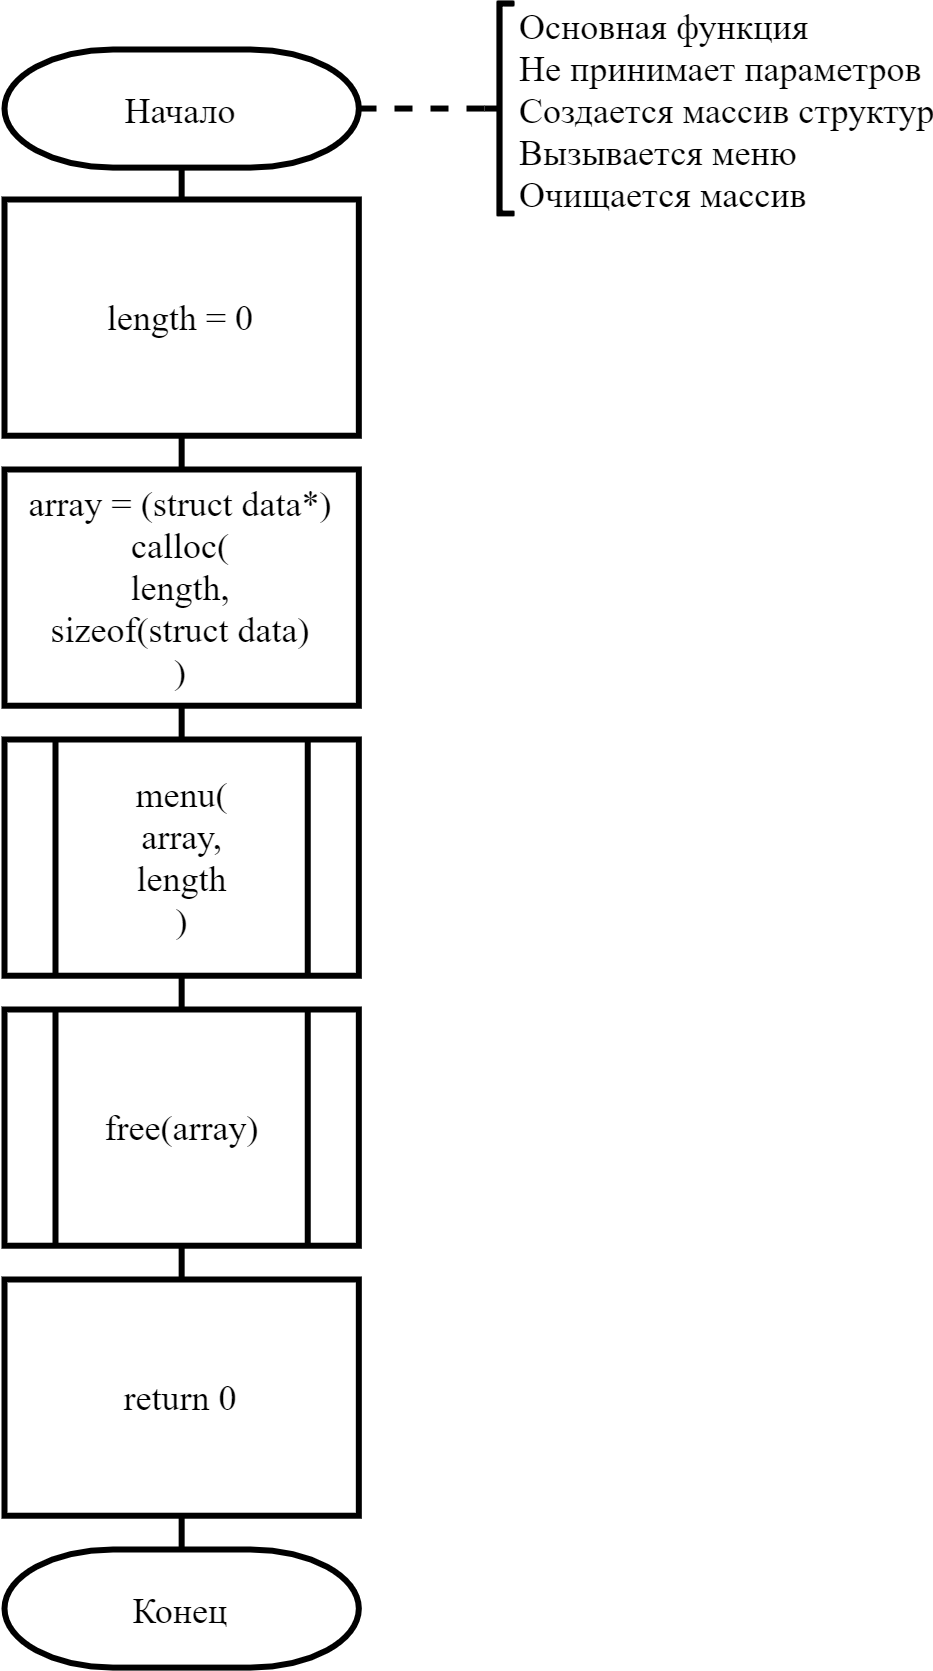
\includegraphics[]{../src/main.png}
    }
    \caption{main()}
\end{figure}

% = = =

\begin{figure}[H]
    \center{
        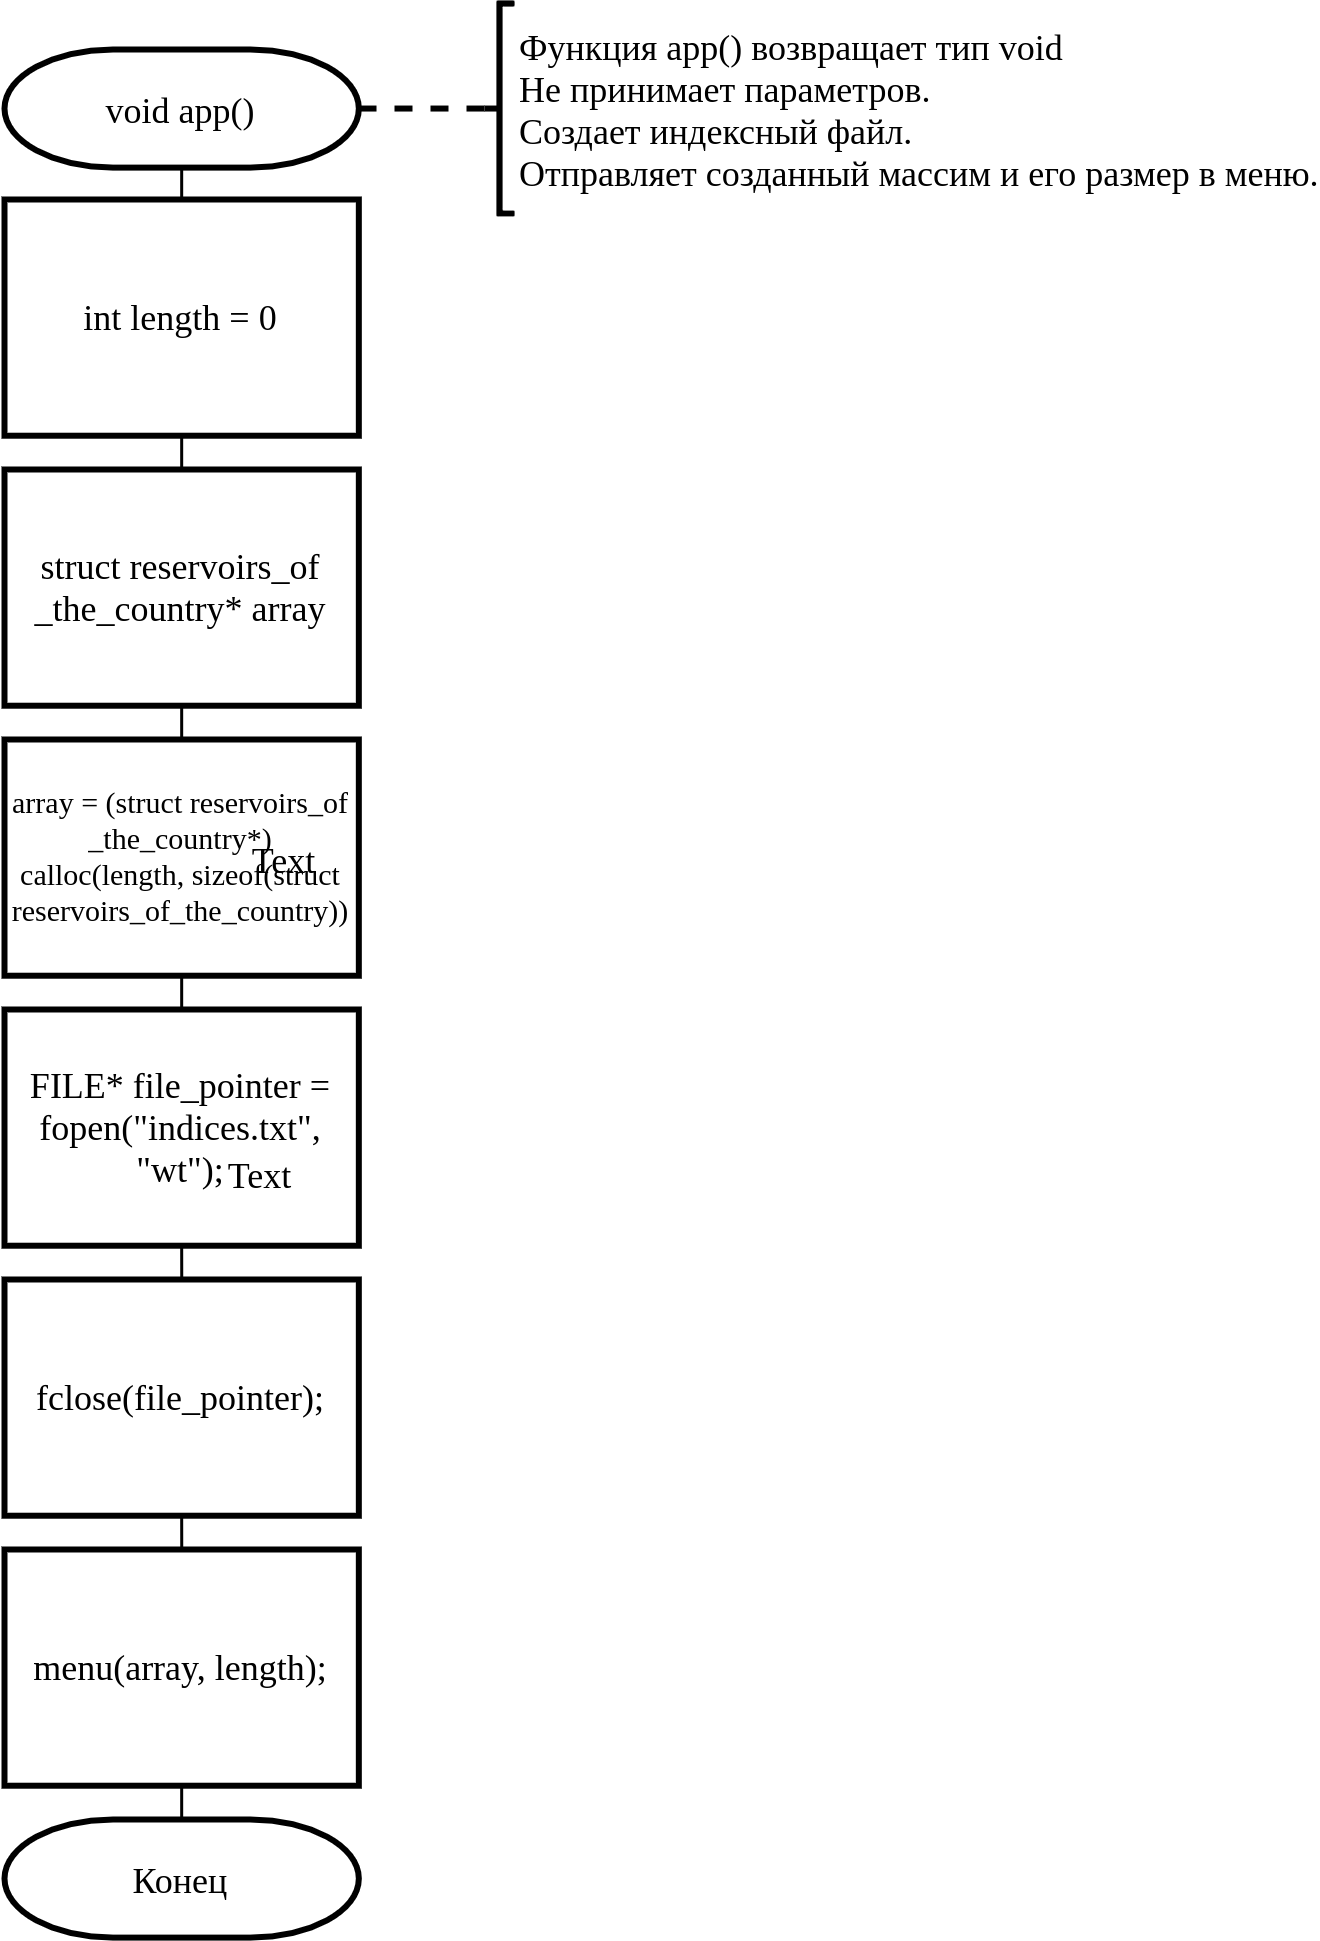
\includegraphics[]{../src/app/app.png}
    }
    \caption{app()}
\end{figure}

% = = =

\begin{figure}[H]
    \center{
        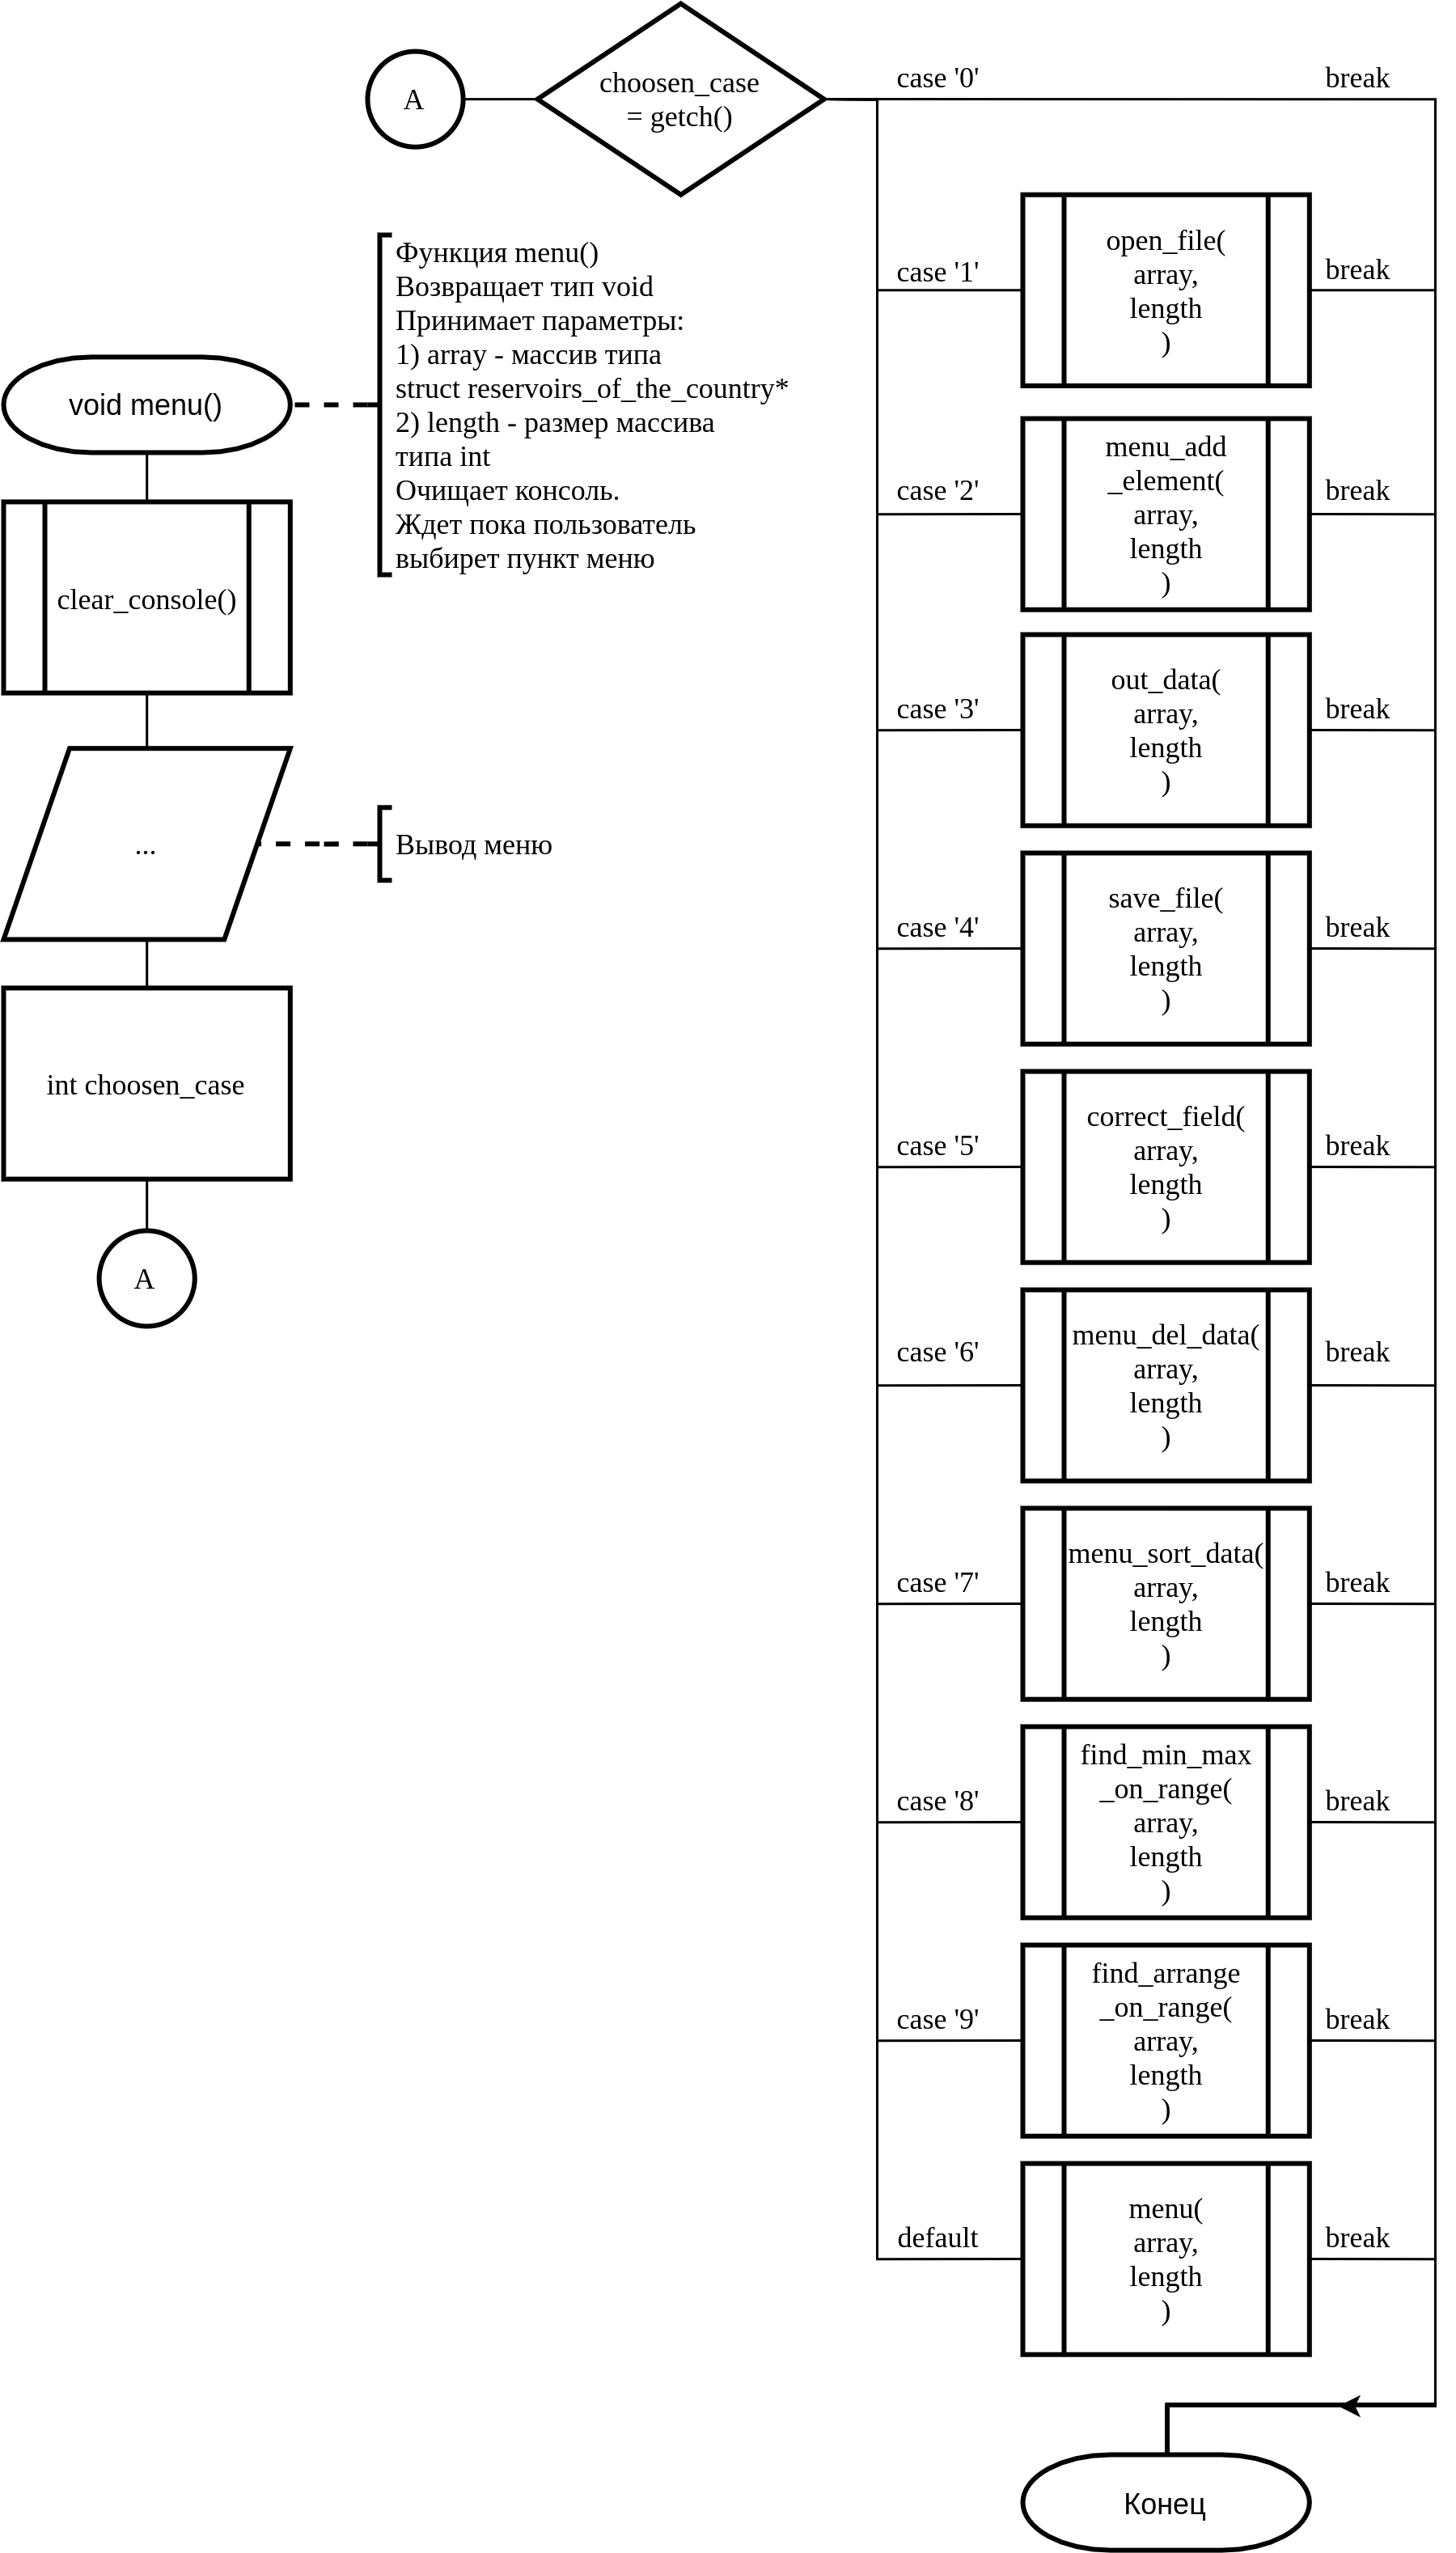
\includegraphics[height=24cm]{../src/app/menu/menu.png}
    }
    \caption{menu()}
\end{figure}

% = = =

\newpage
\section{Свои библиотеки}

% = = =

\begin{figure}[H]
    \center{
        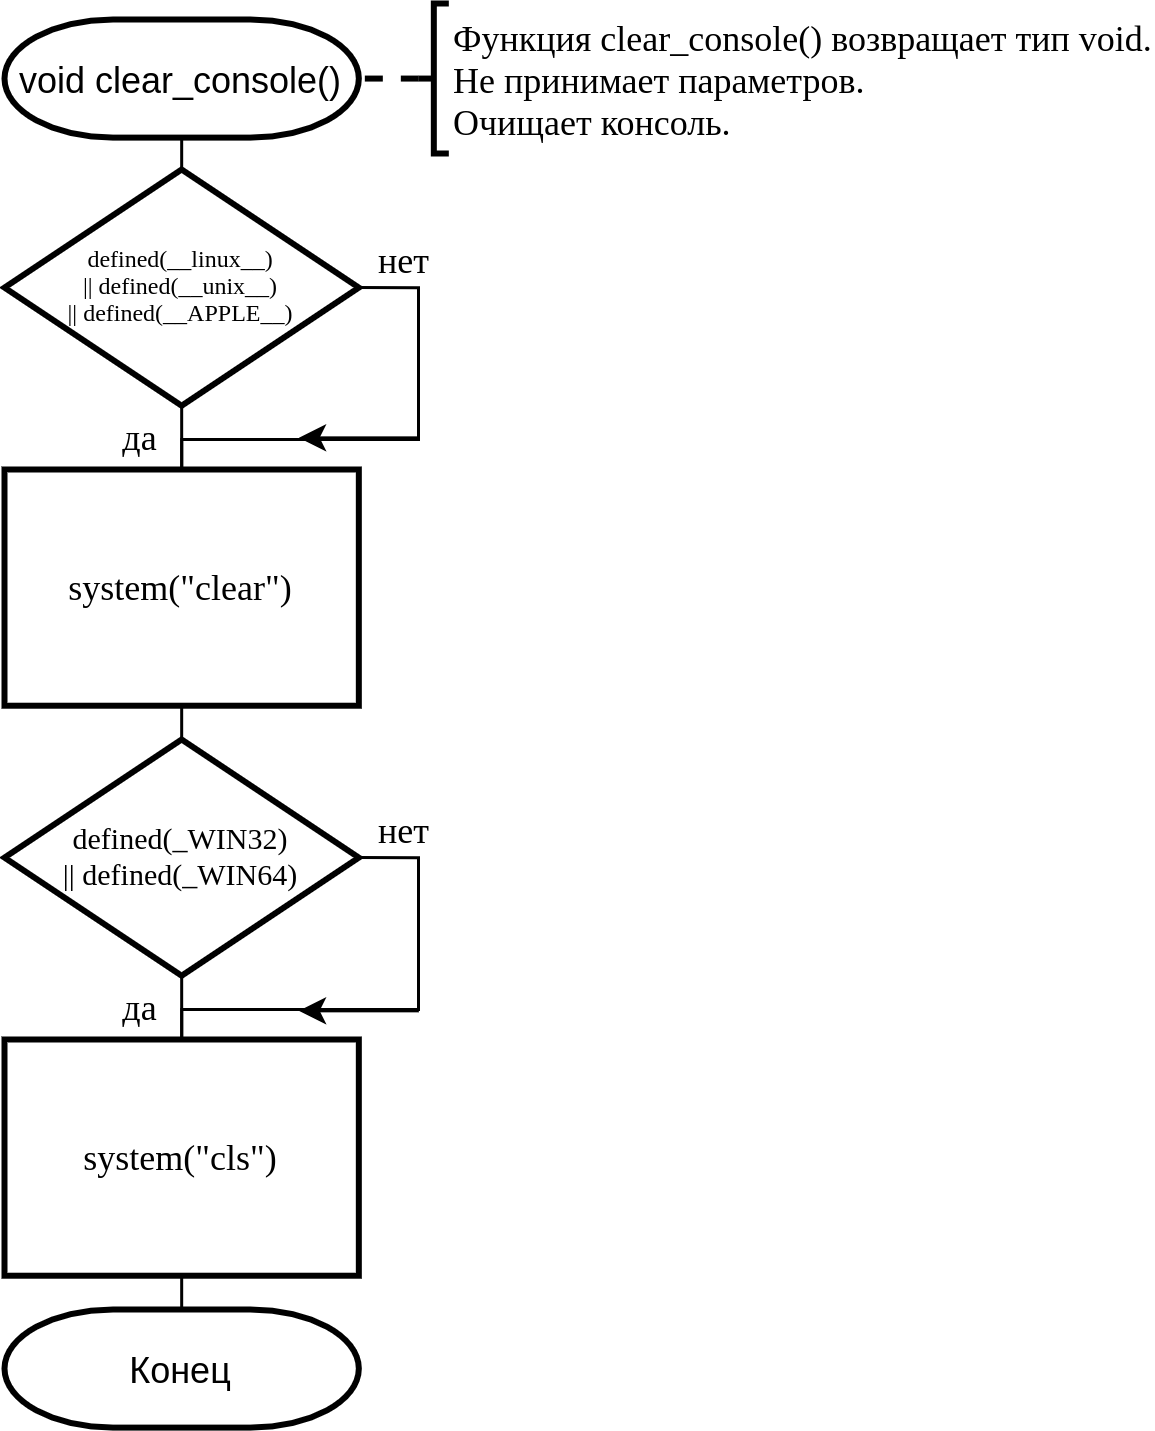
\includegraphics[]{../src/my_libs/clear_console/clear_console.png}
    }
    \caption{clear\_console()}
\end{figure}

% = = =

%getch()

% = = =

\begin{figure}[H]
    \center{
        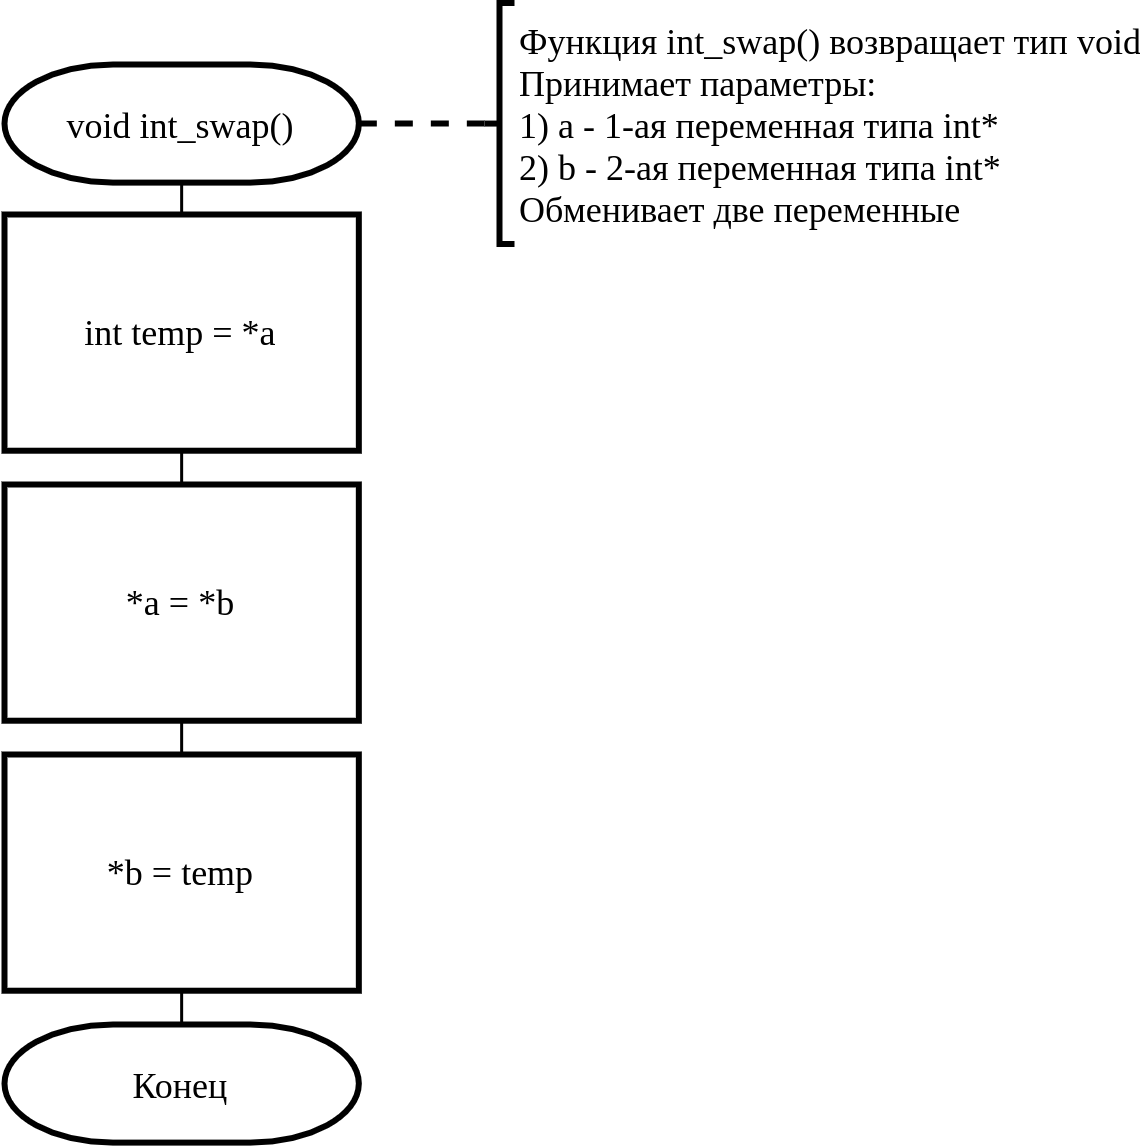
\includegraphics[]{../src/my_libs/int_swap/int_swap.png}
    }
    \caption{int\_swap()}
\end{figure}

% = = =

\begin{figure}[H]
    \center{
        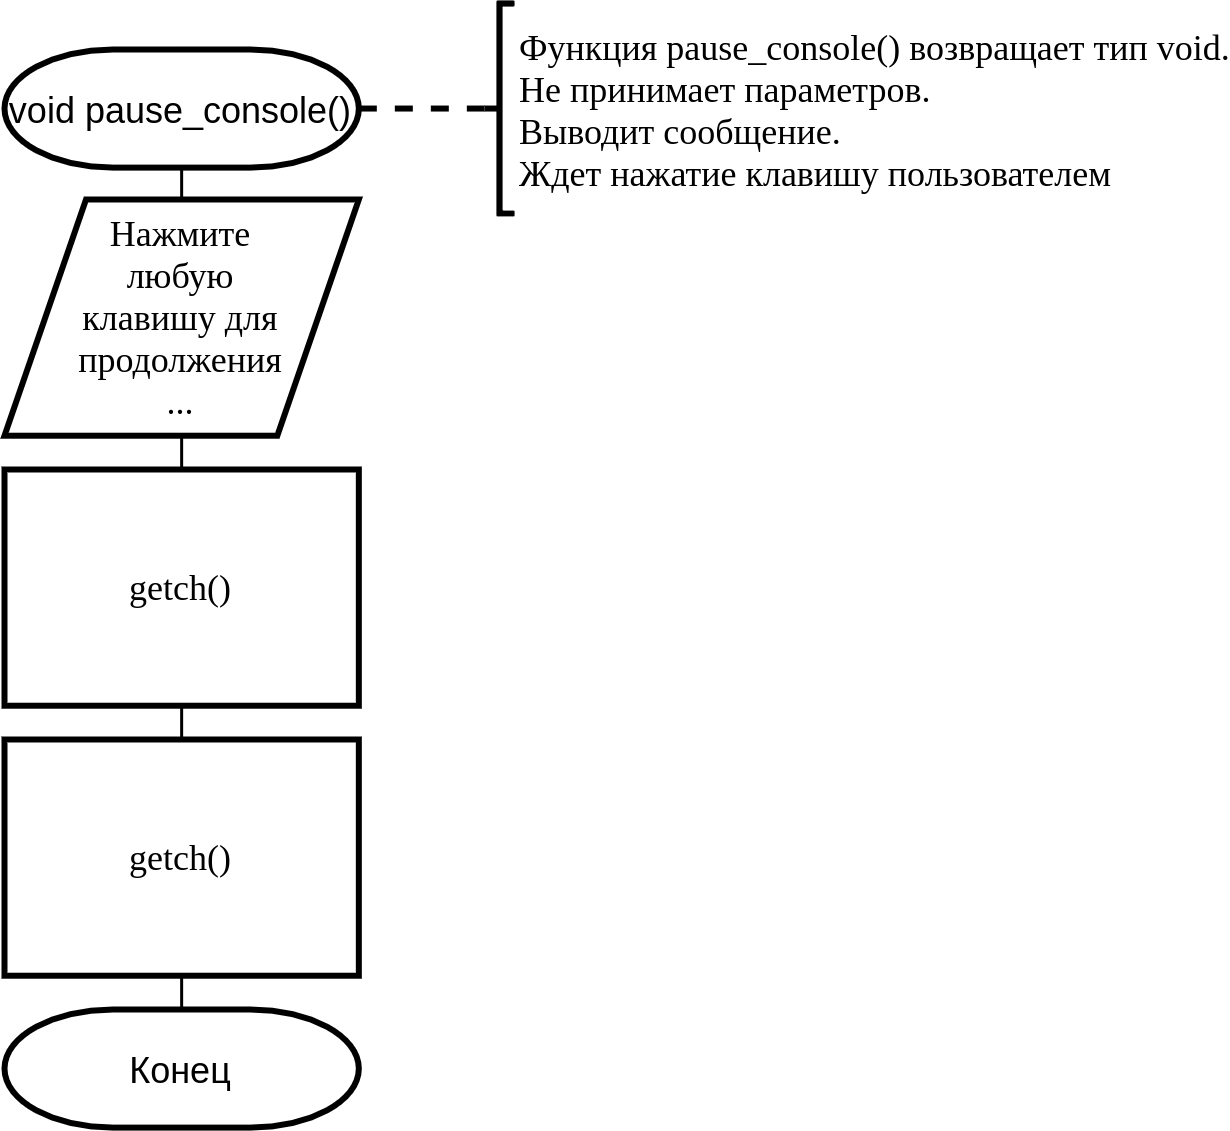
\includegraphics[]{../src/my_libs/pause_console/pause_console.png}
    }
    \caption{pause\_console()}
\end{figure}

% = = =

\begin{figure}[H]
    \center{
        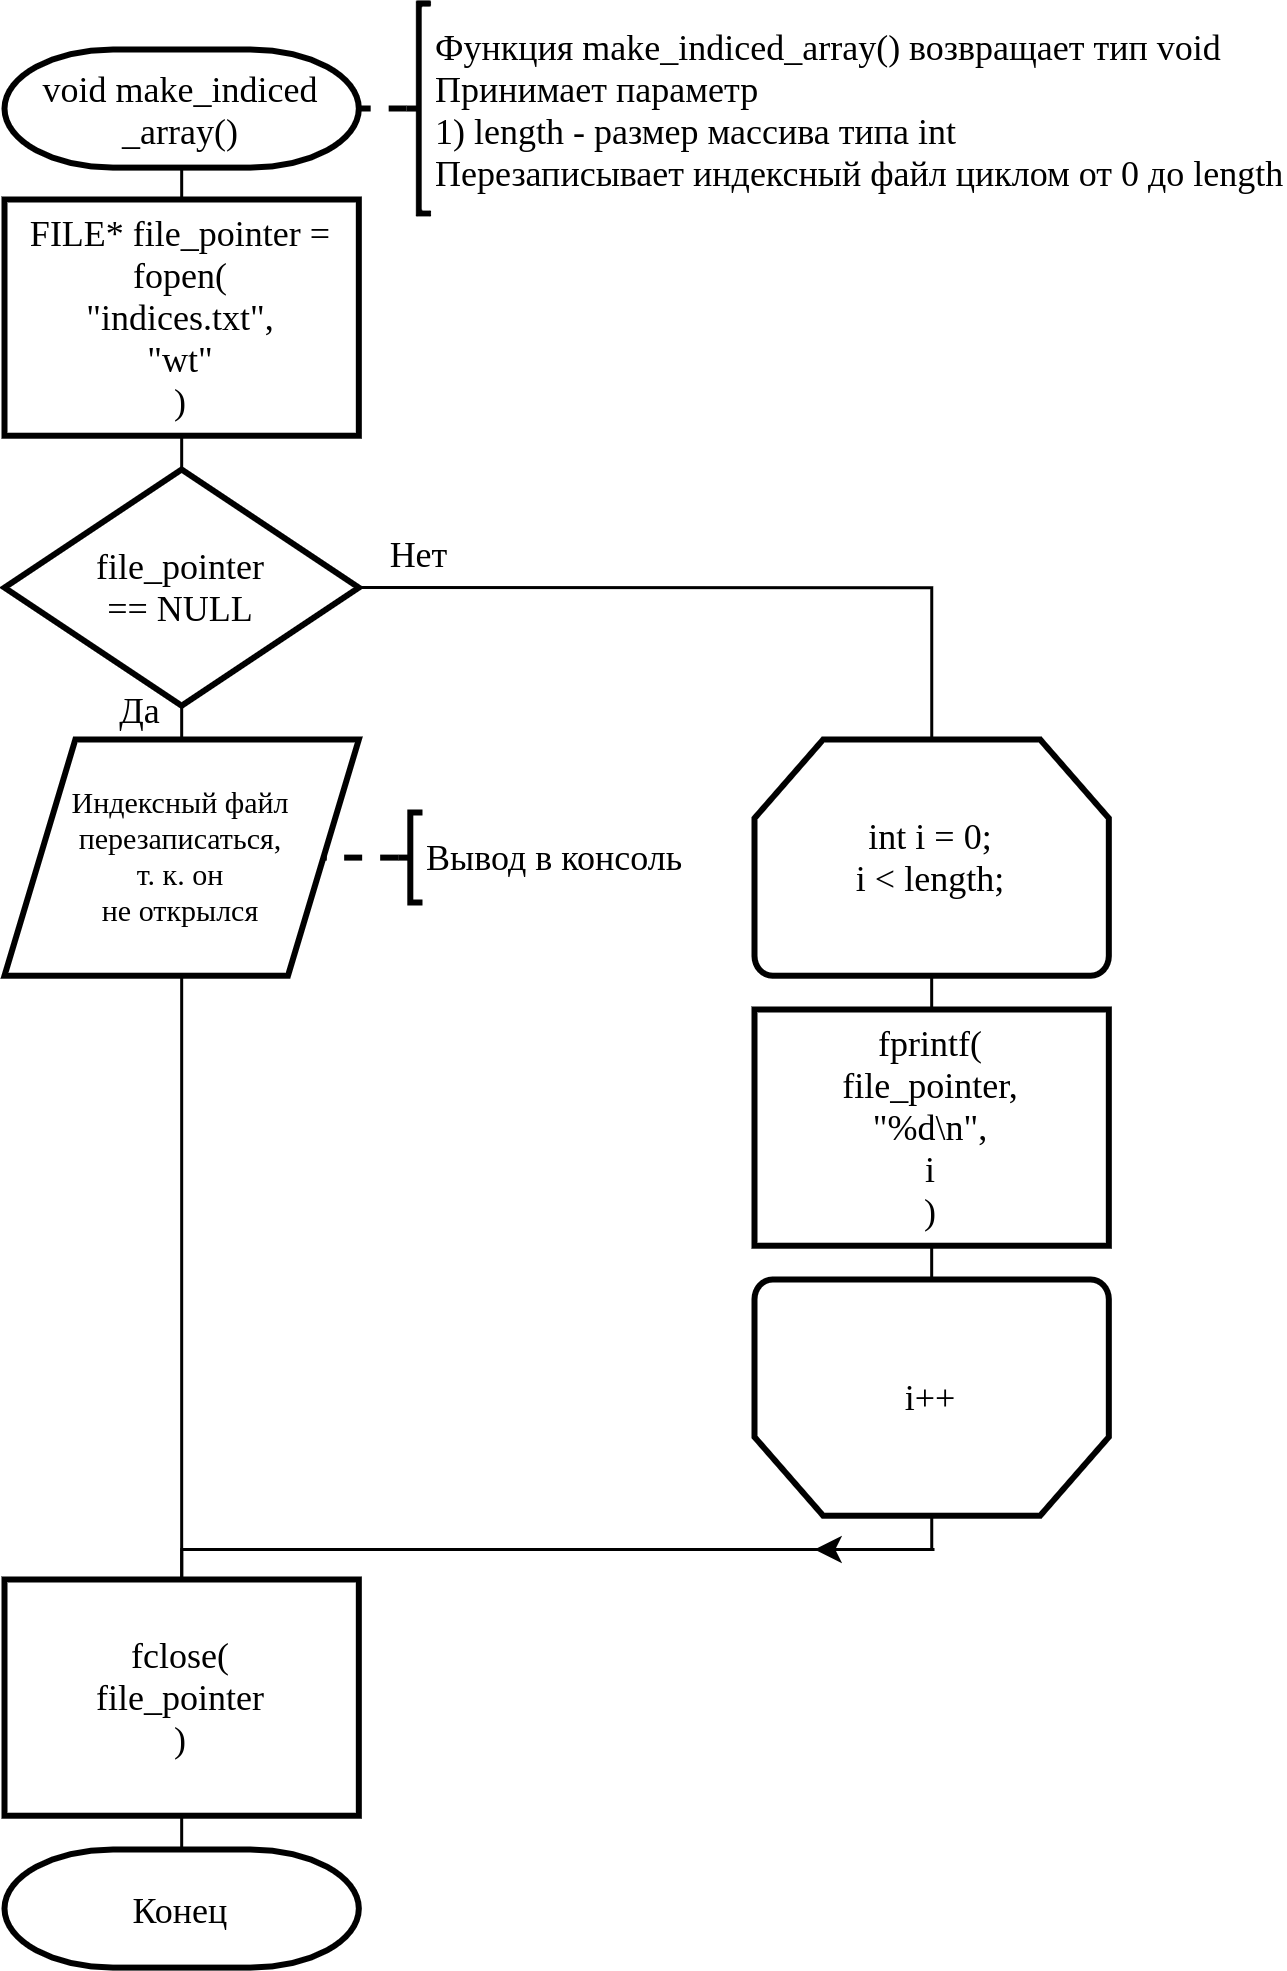
\includegraphics[]{../src/my_libs/indices_array/make_indiced_array.png}
    }
    \caption{make\_indiced\_array()}
\end{figure}

% = = =

\begin{figure}[H]
    \center{
        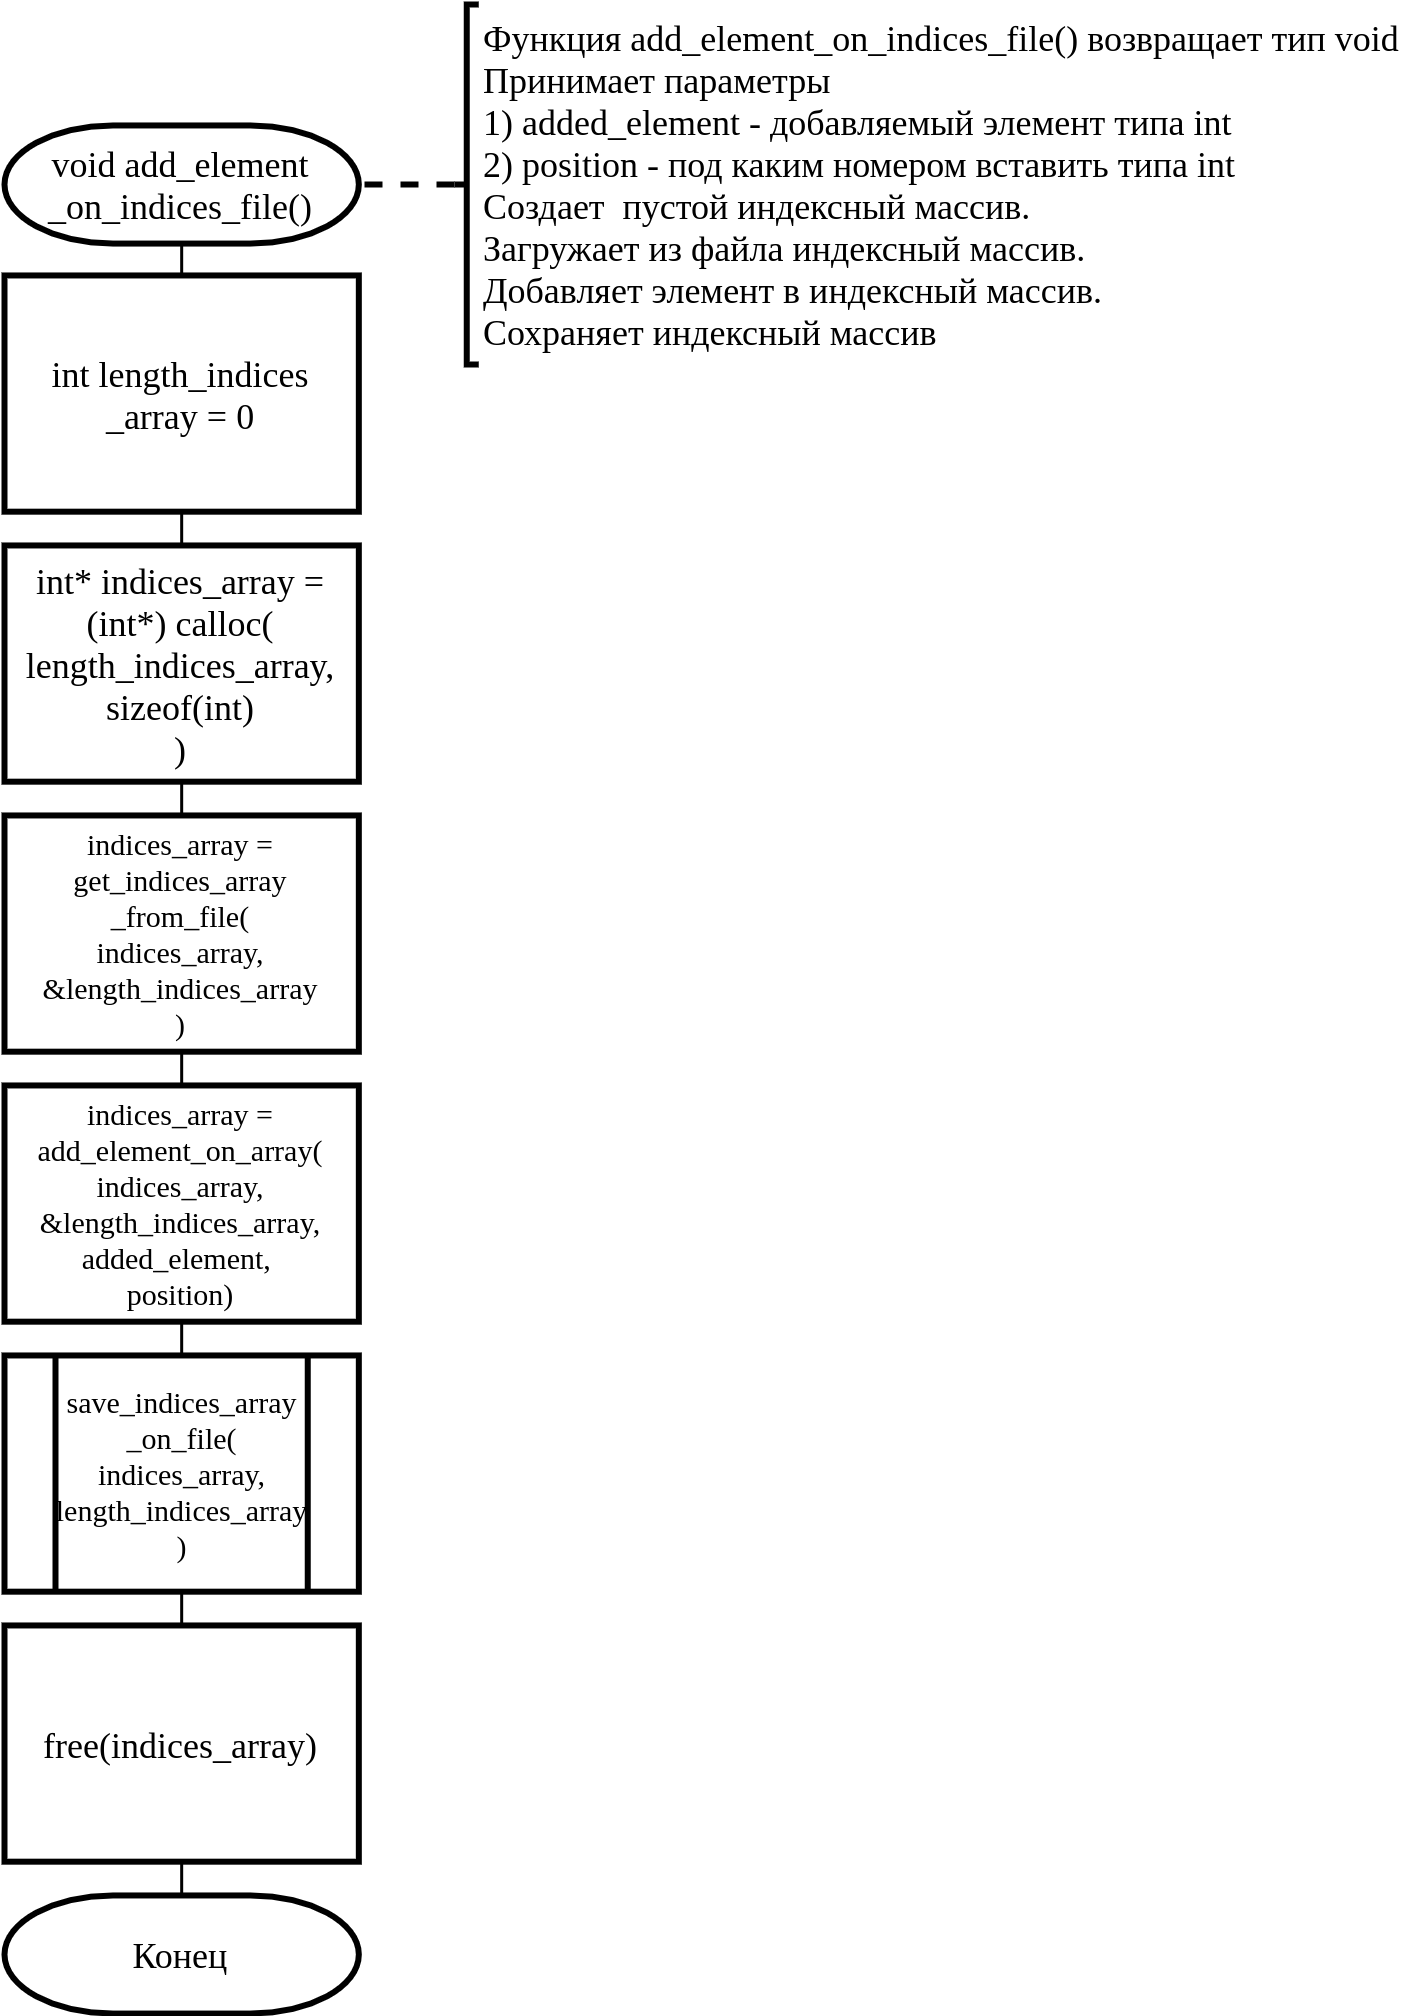
\includegraphics[]{../src/my_libs/indices_array/add_element_on_indices_array.png}
    }
    \caption{add\_element\_on\_indices\_array()}
\end{figure}

% = = =

\begin{figure}[H]
    \center{
        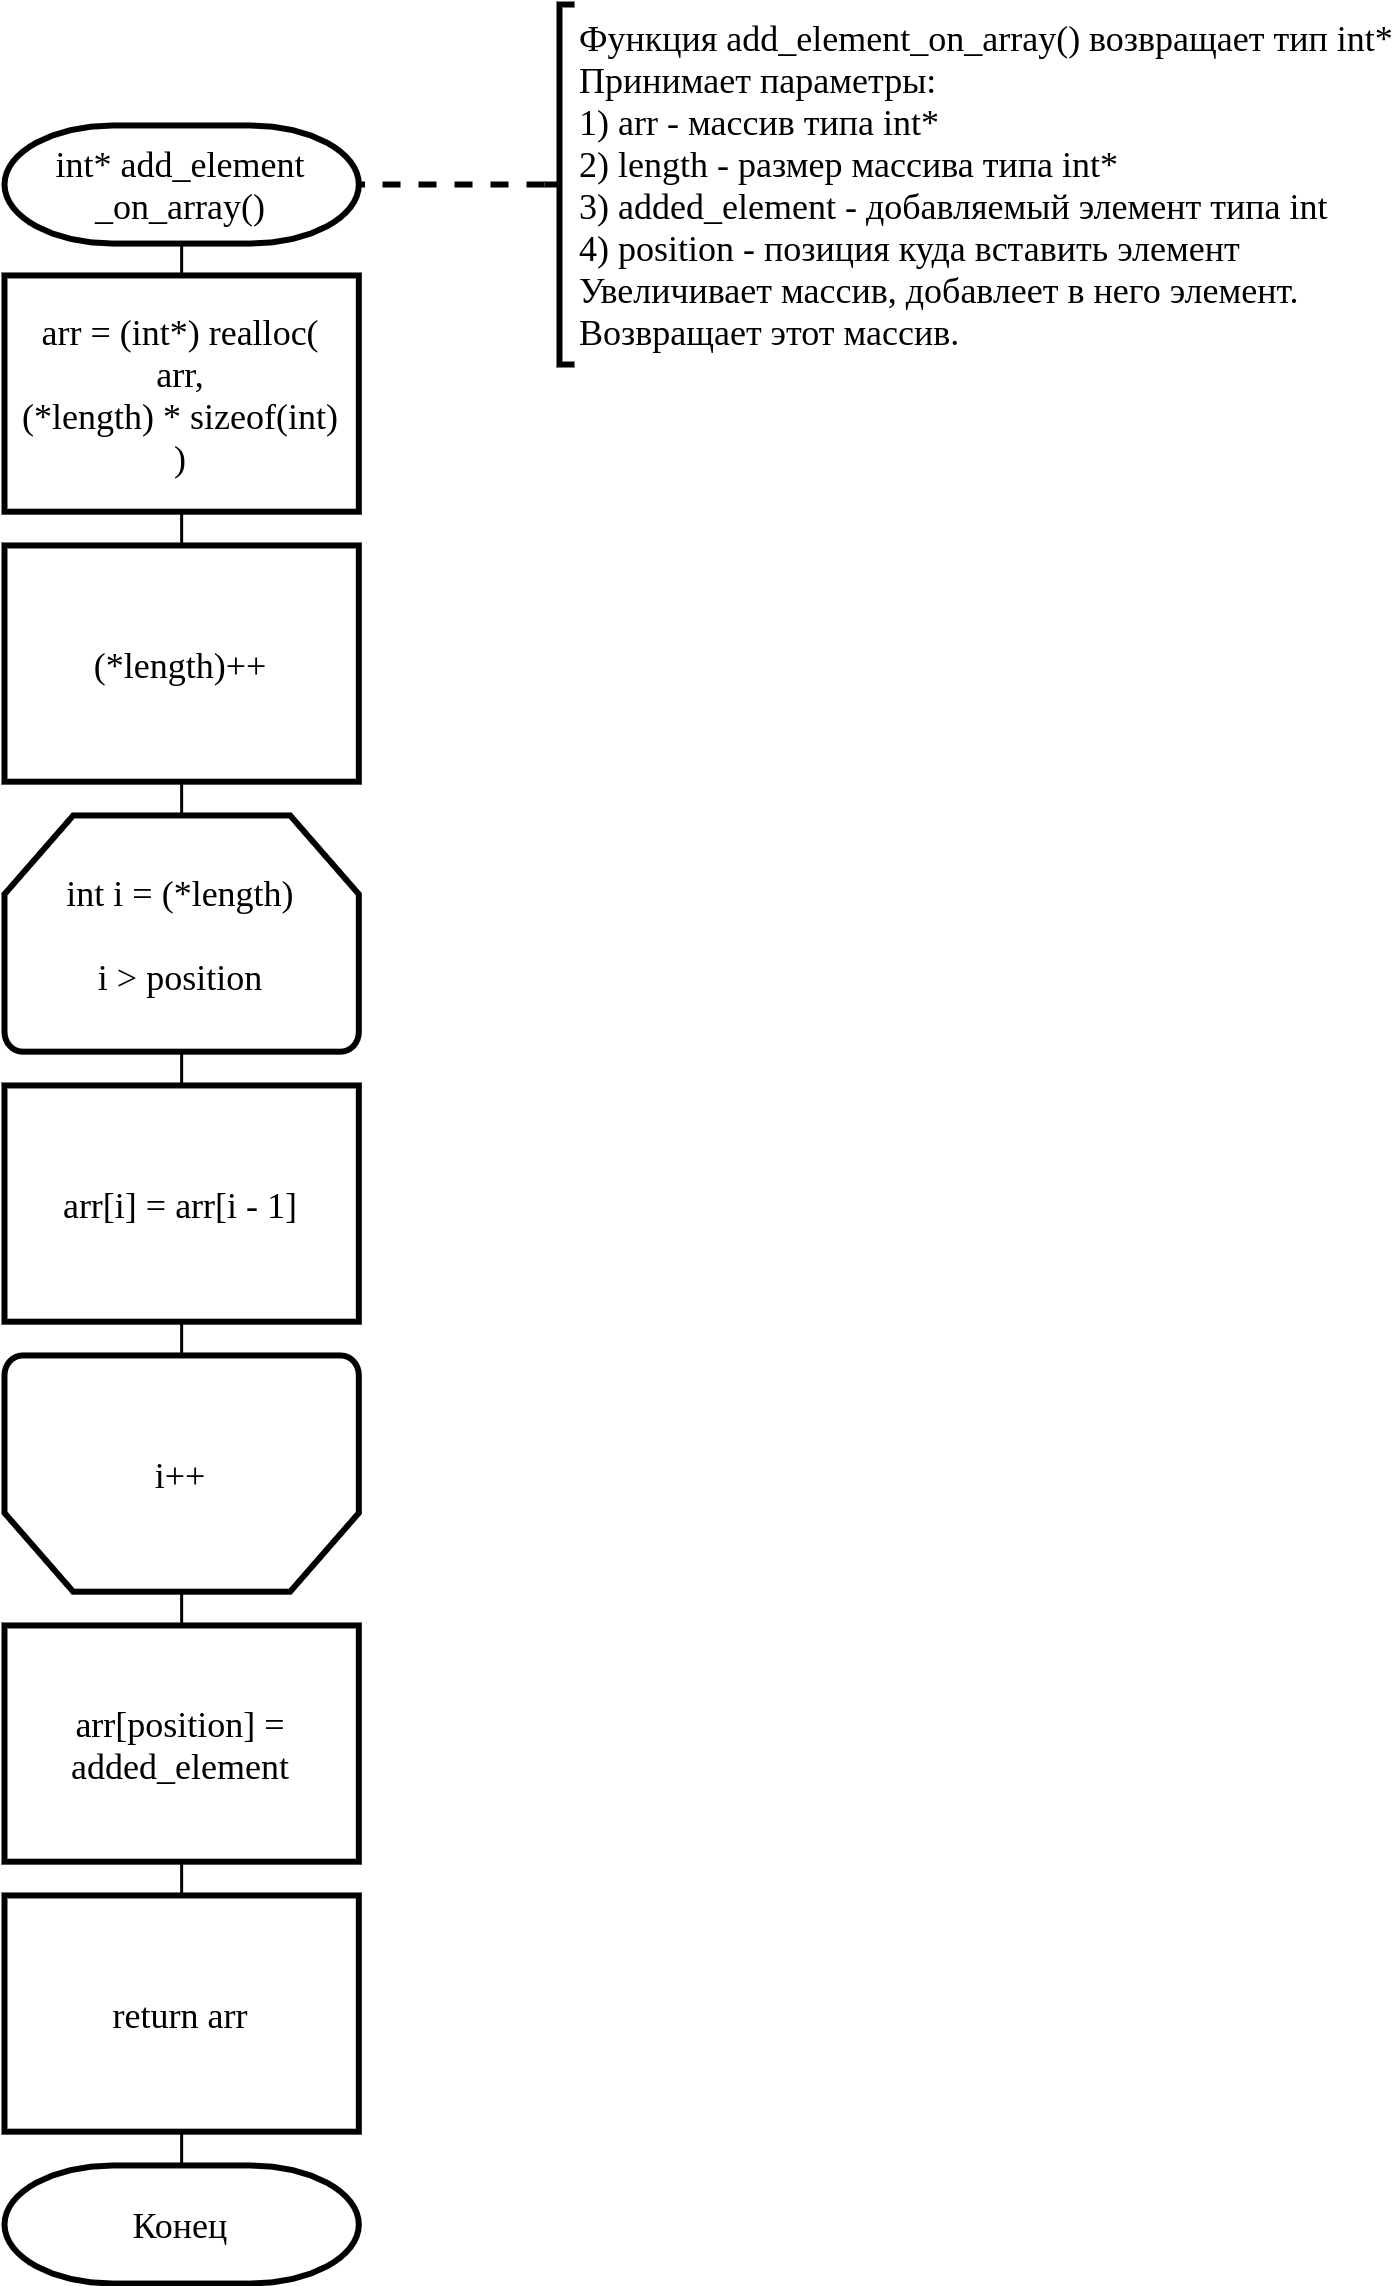
\includegraphics[]{../src/my_libs/indices_array/add_element_on_array/add_element_on_array.png}
    }
    \caption{add\_element\_on\_array()}
\end{figure}

% = = =

\begin{figure}[H]
    \center{
        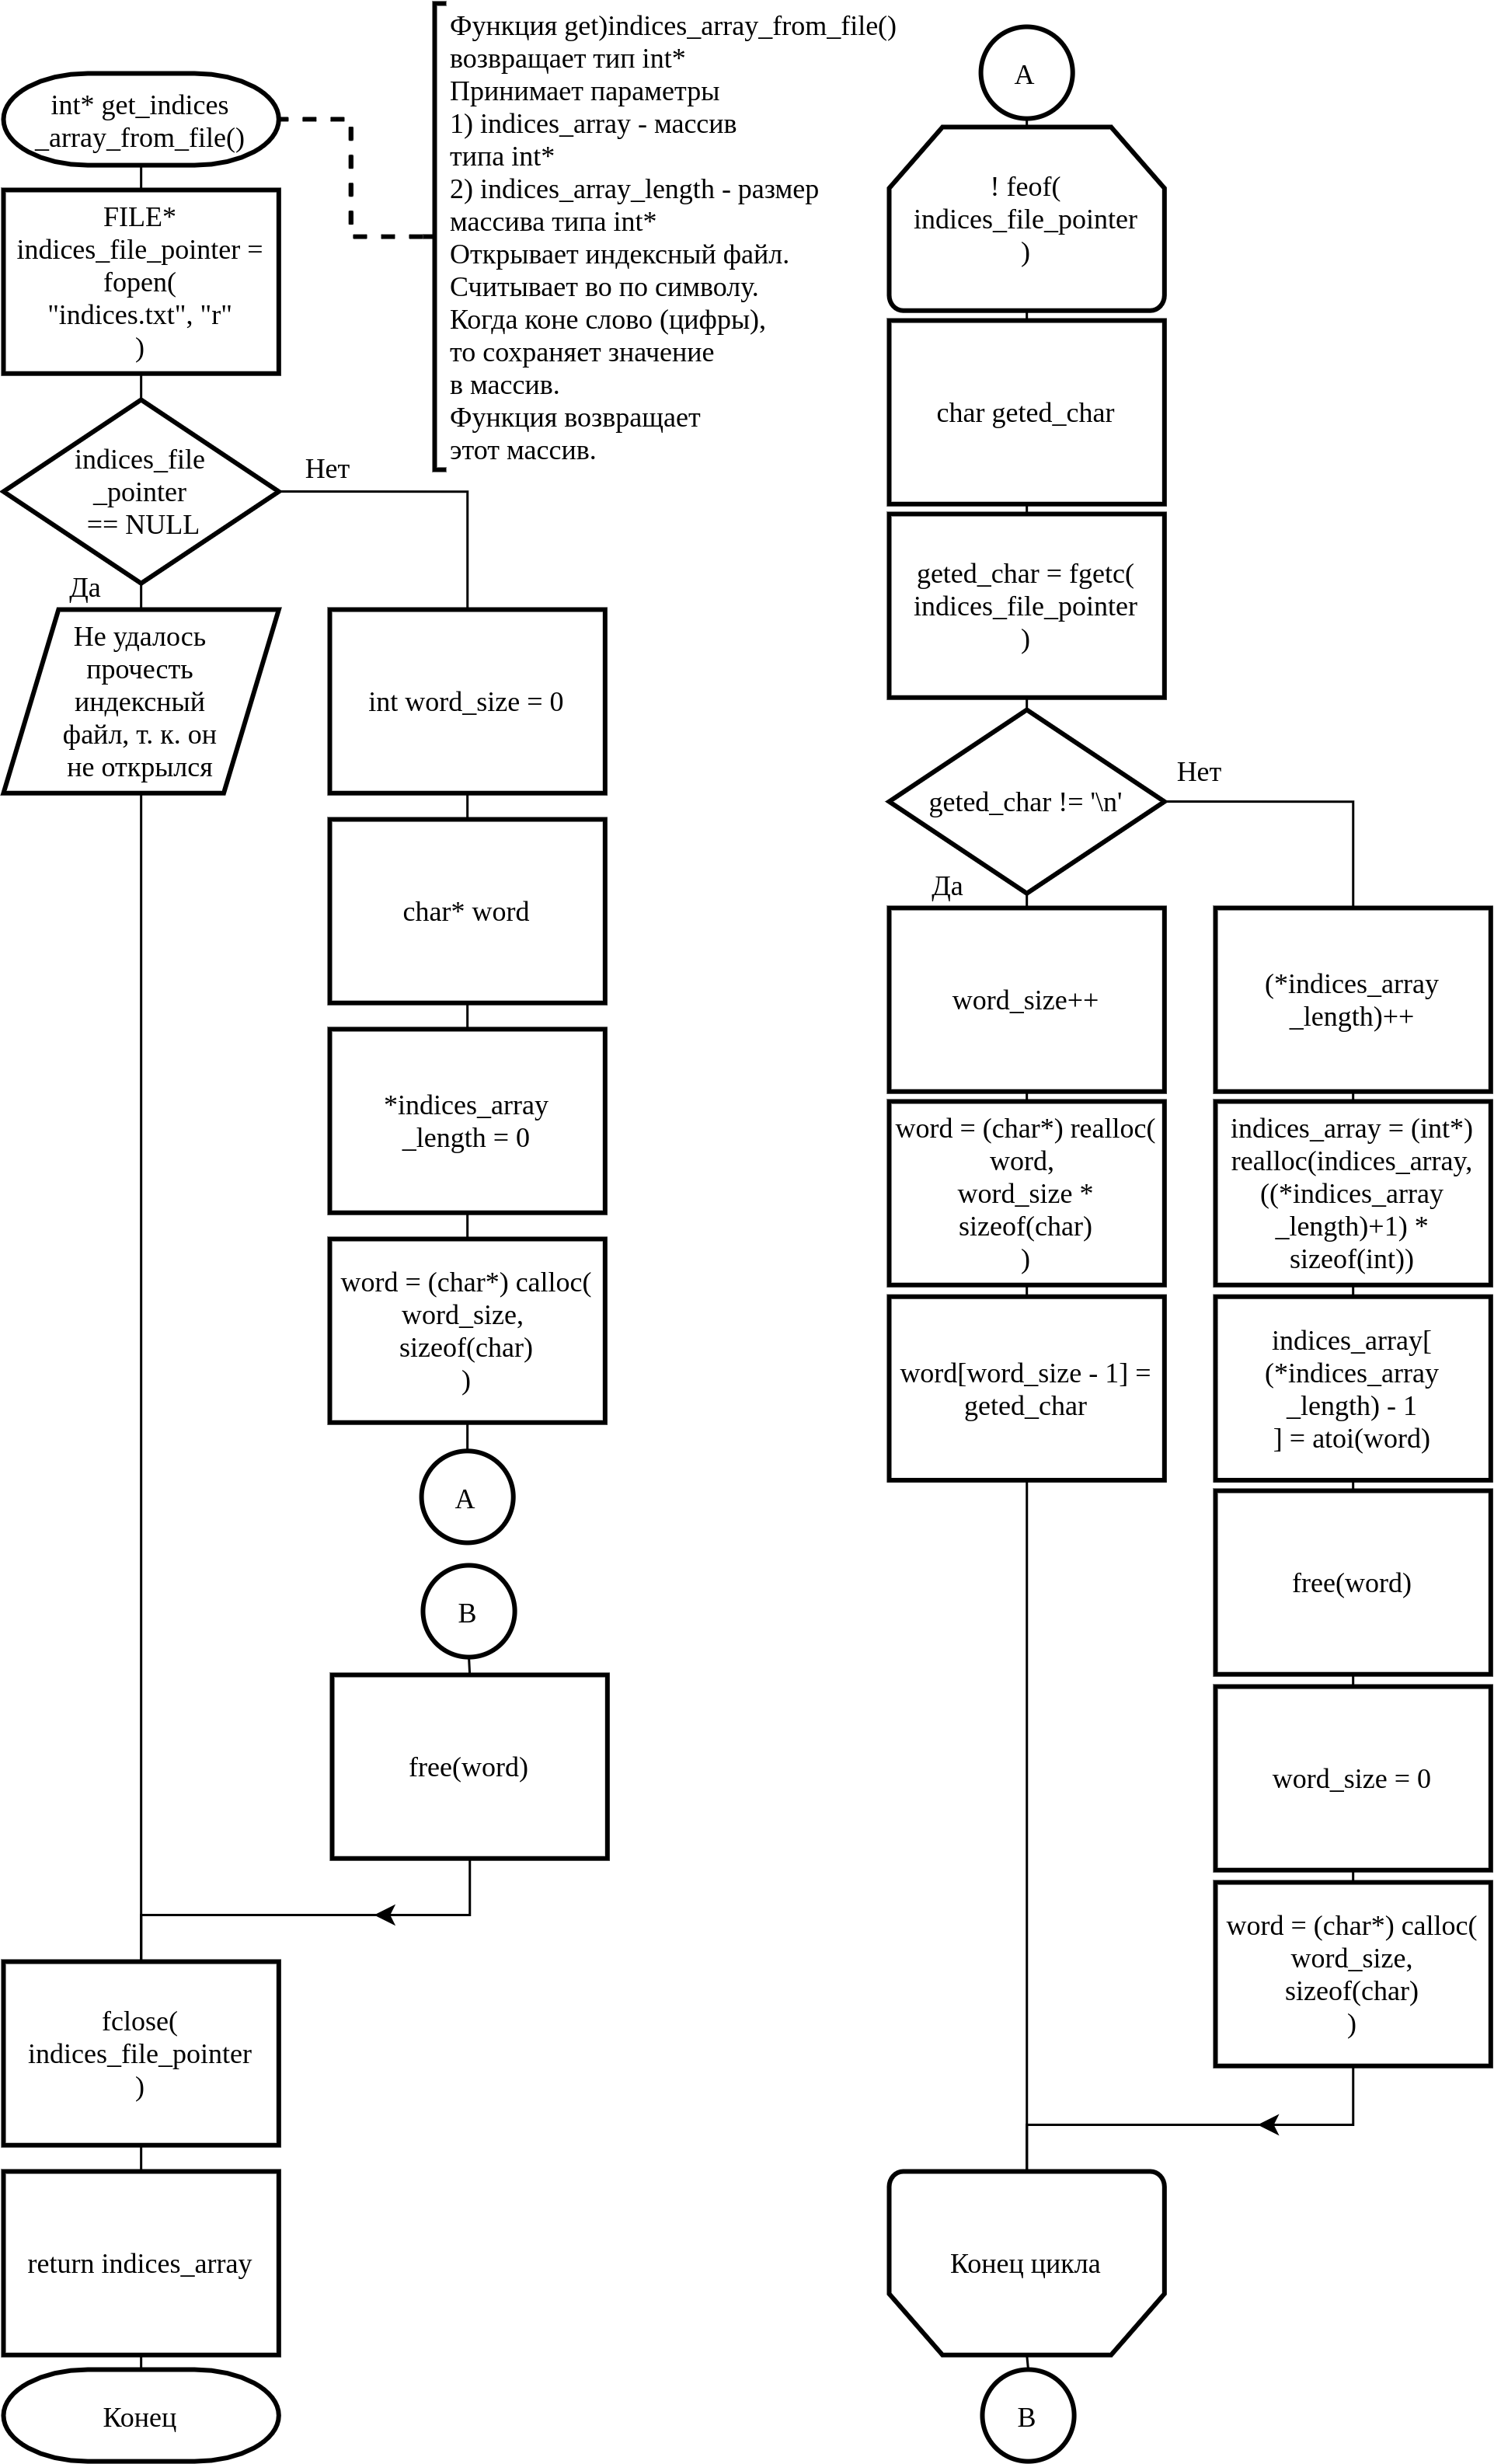
\includegraphics[height = 24cm]{../src/my_libs/indices_array/get_indices_array_from_file/get_indices_array_from_file.png}
    }
    \caption{get\_indices\_array\_from\_file()}
\end{figure}

% = = =

\begin{figure}[H]
    \center{
        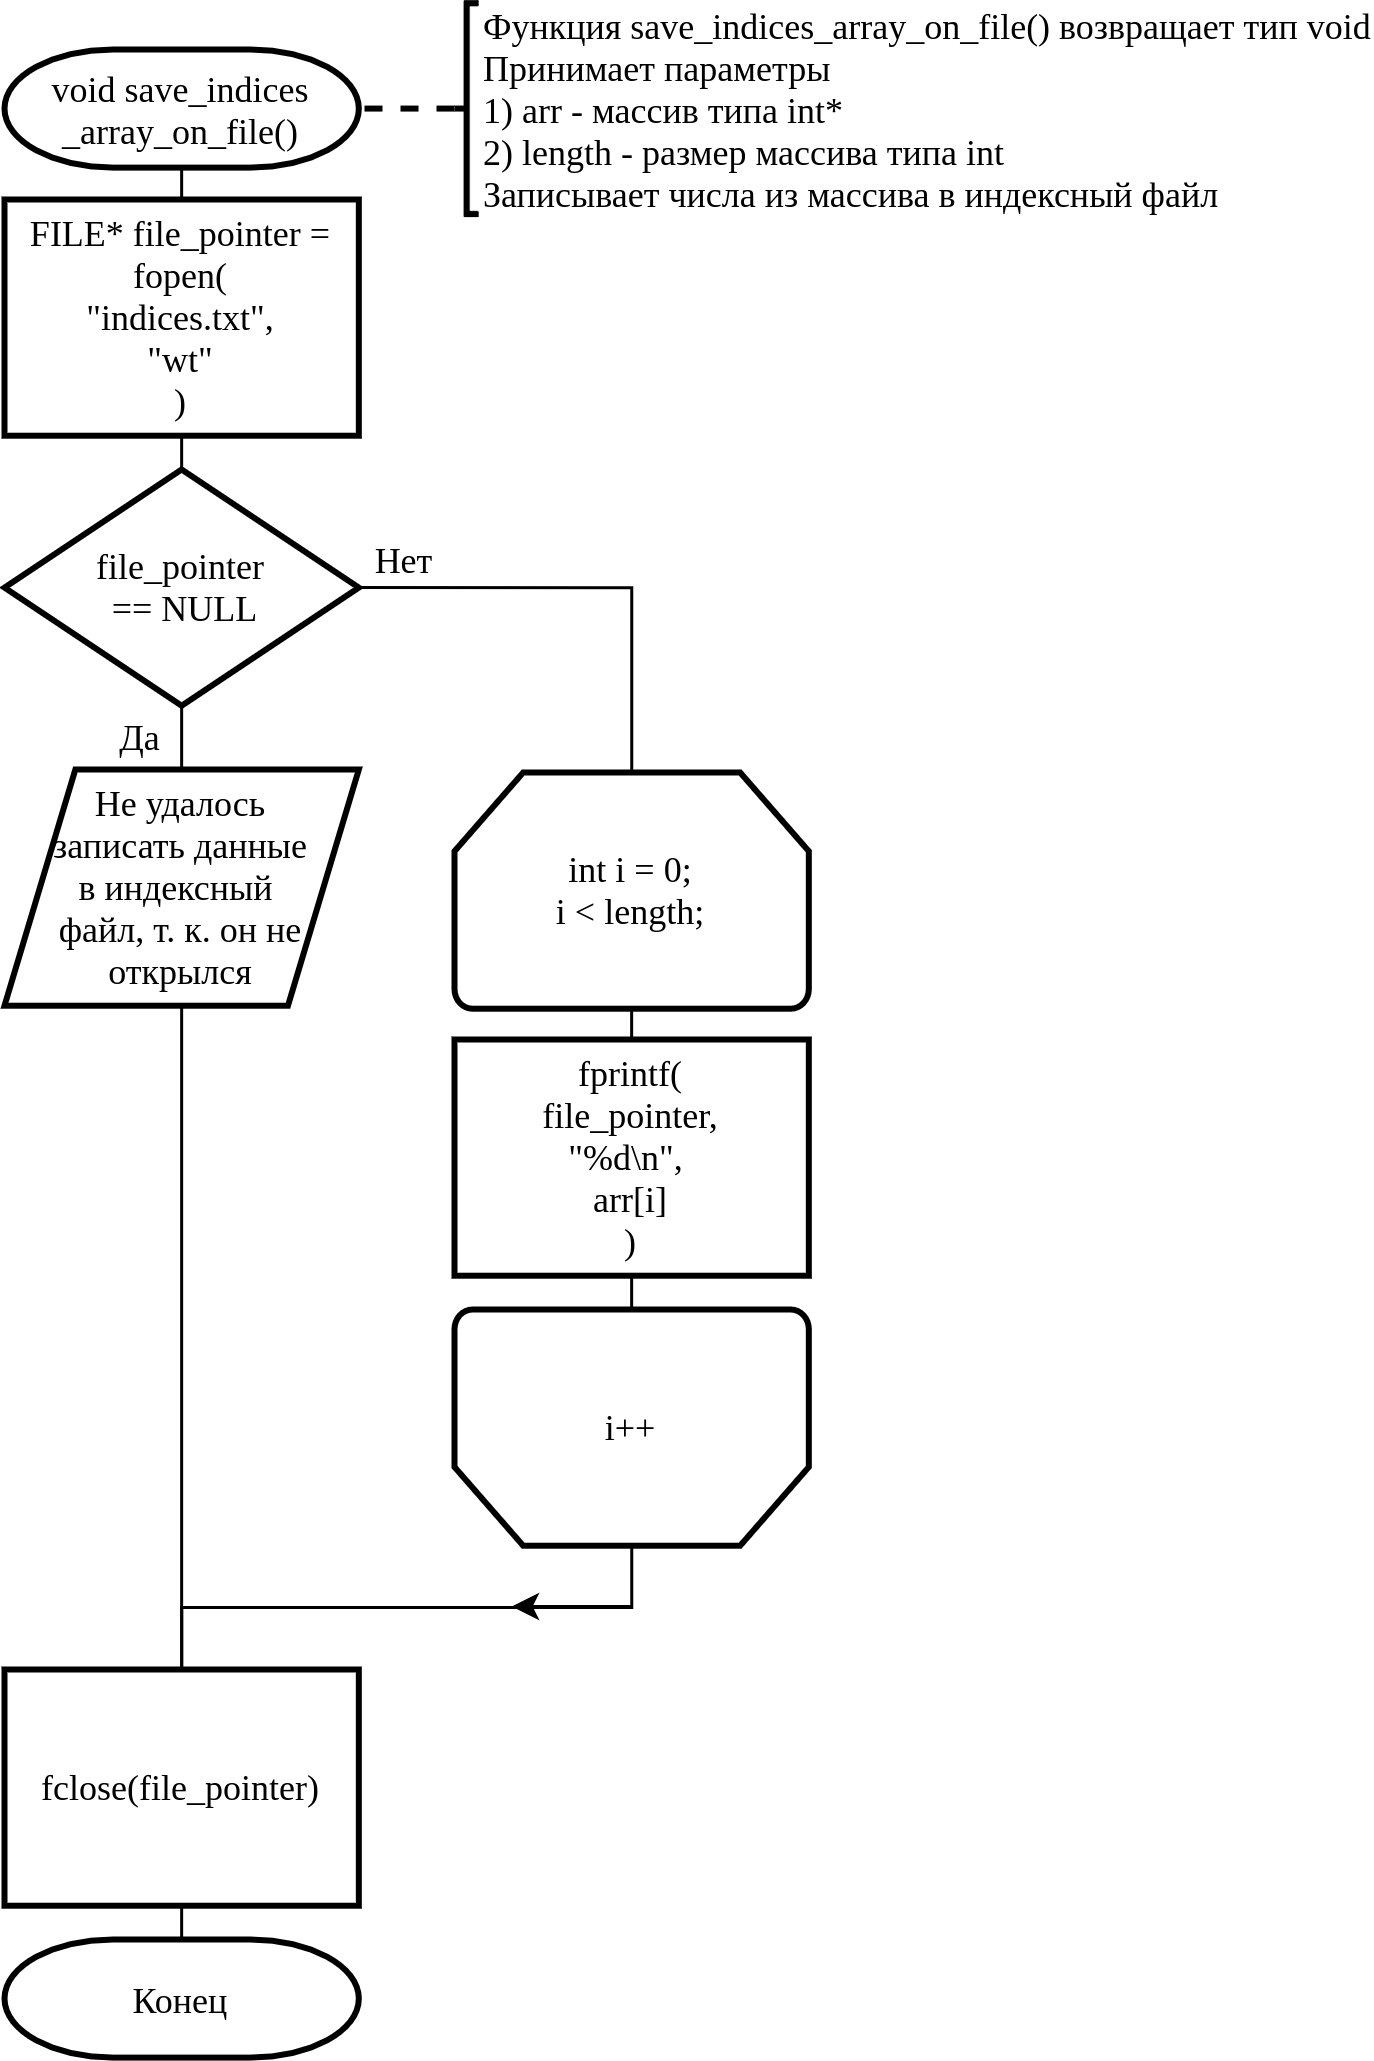
\includegraphics[]{../src/my_libs/indices_array/save_indices_array_on_file/save_indices_array_on_file.png}
    }
    \caption{save\_indices\_array\_on\_file()}
\end{figure}

% = = =

\newpage
\section{Открытие файла}

% = = =

\begin{figure}[H]
    \center{
        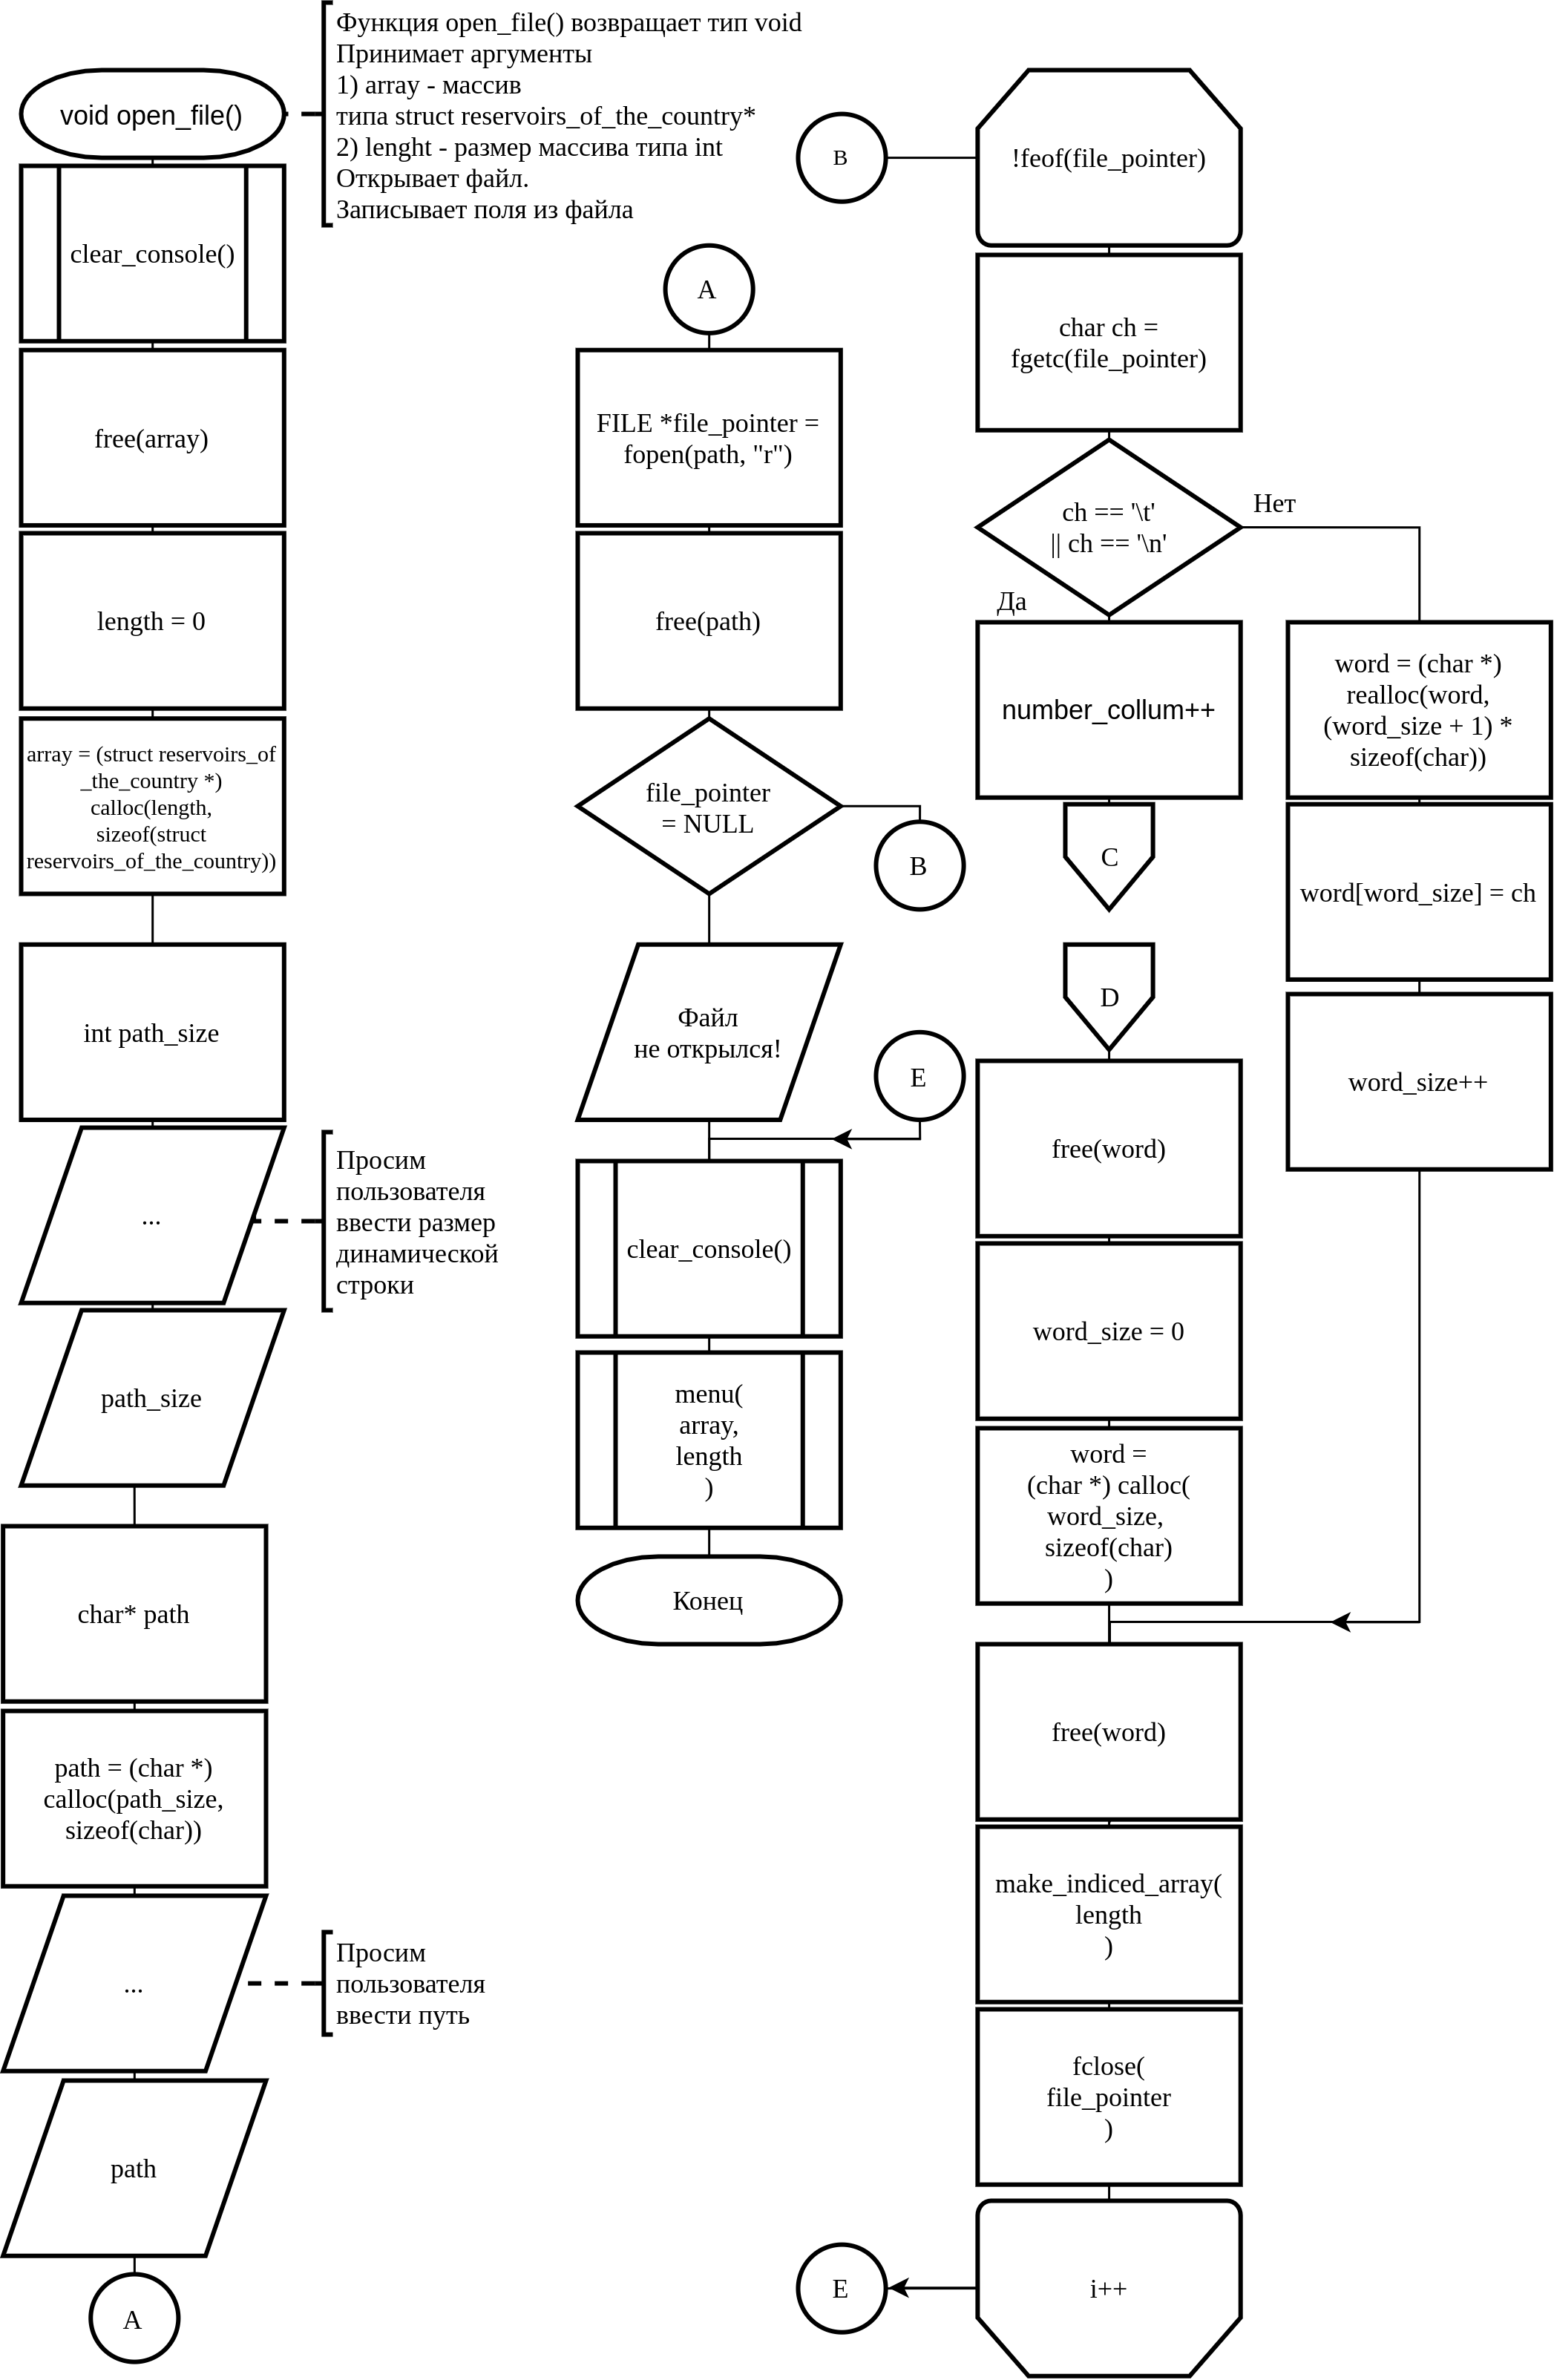
\includegraphics[height=24cm]{../src/app/menu/open_file/open_file-Page-1.png}
    }
    \caption{open\_file() часть 1}
\end{figure}

\begin{figure}[H]
    \center{
        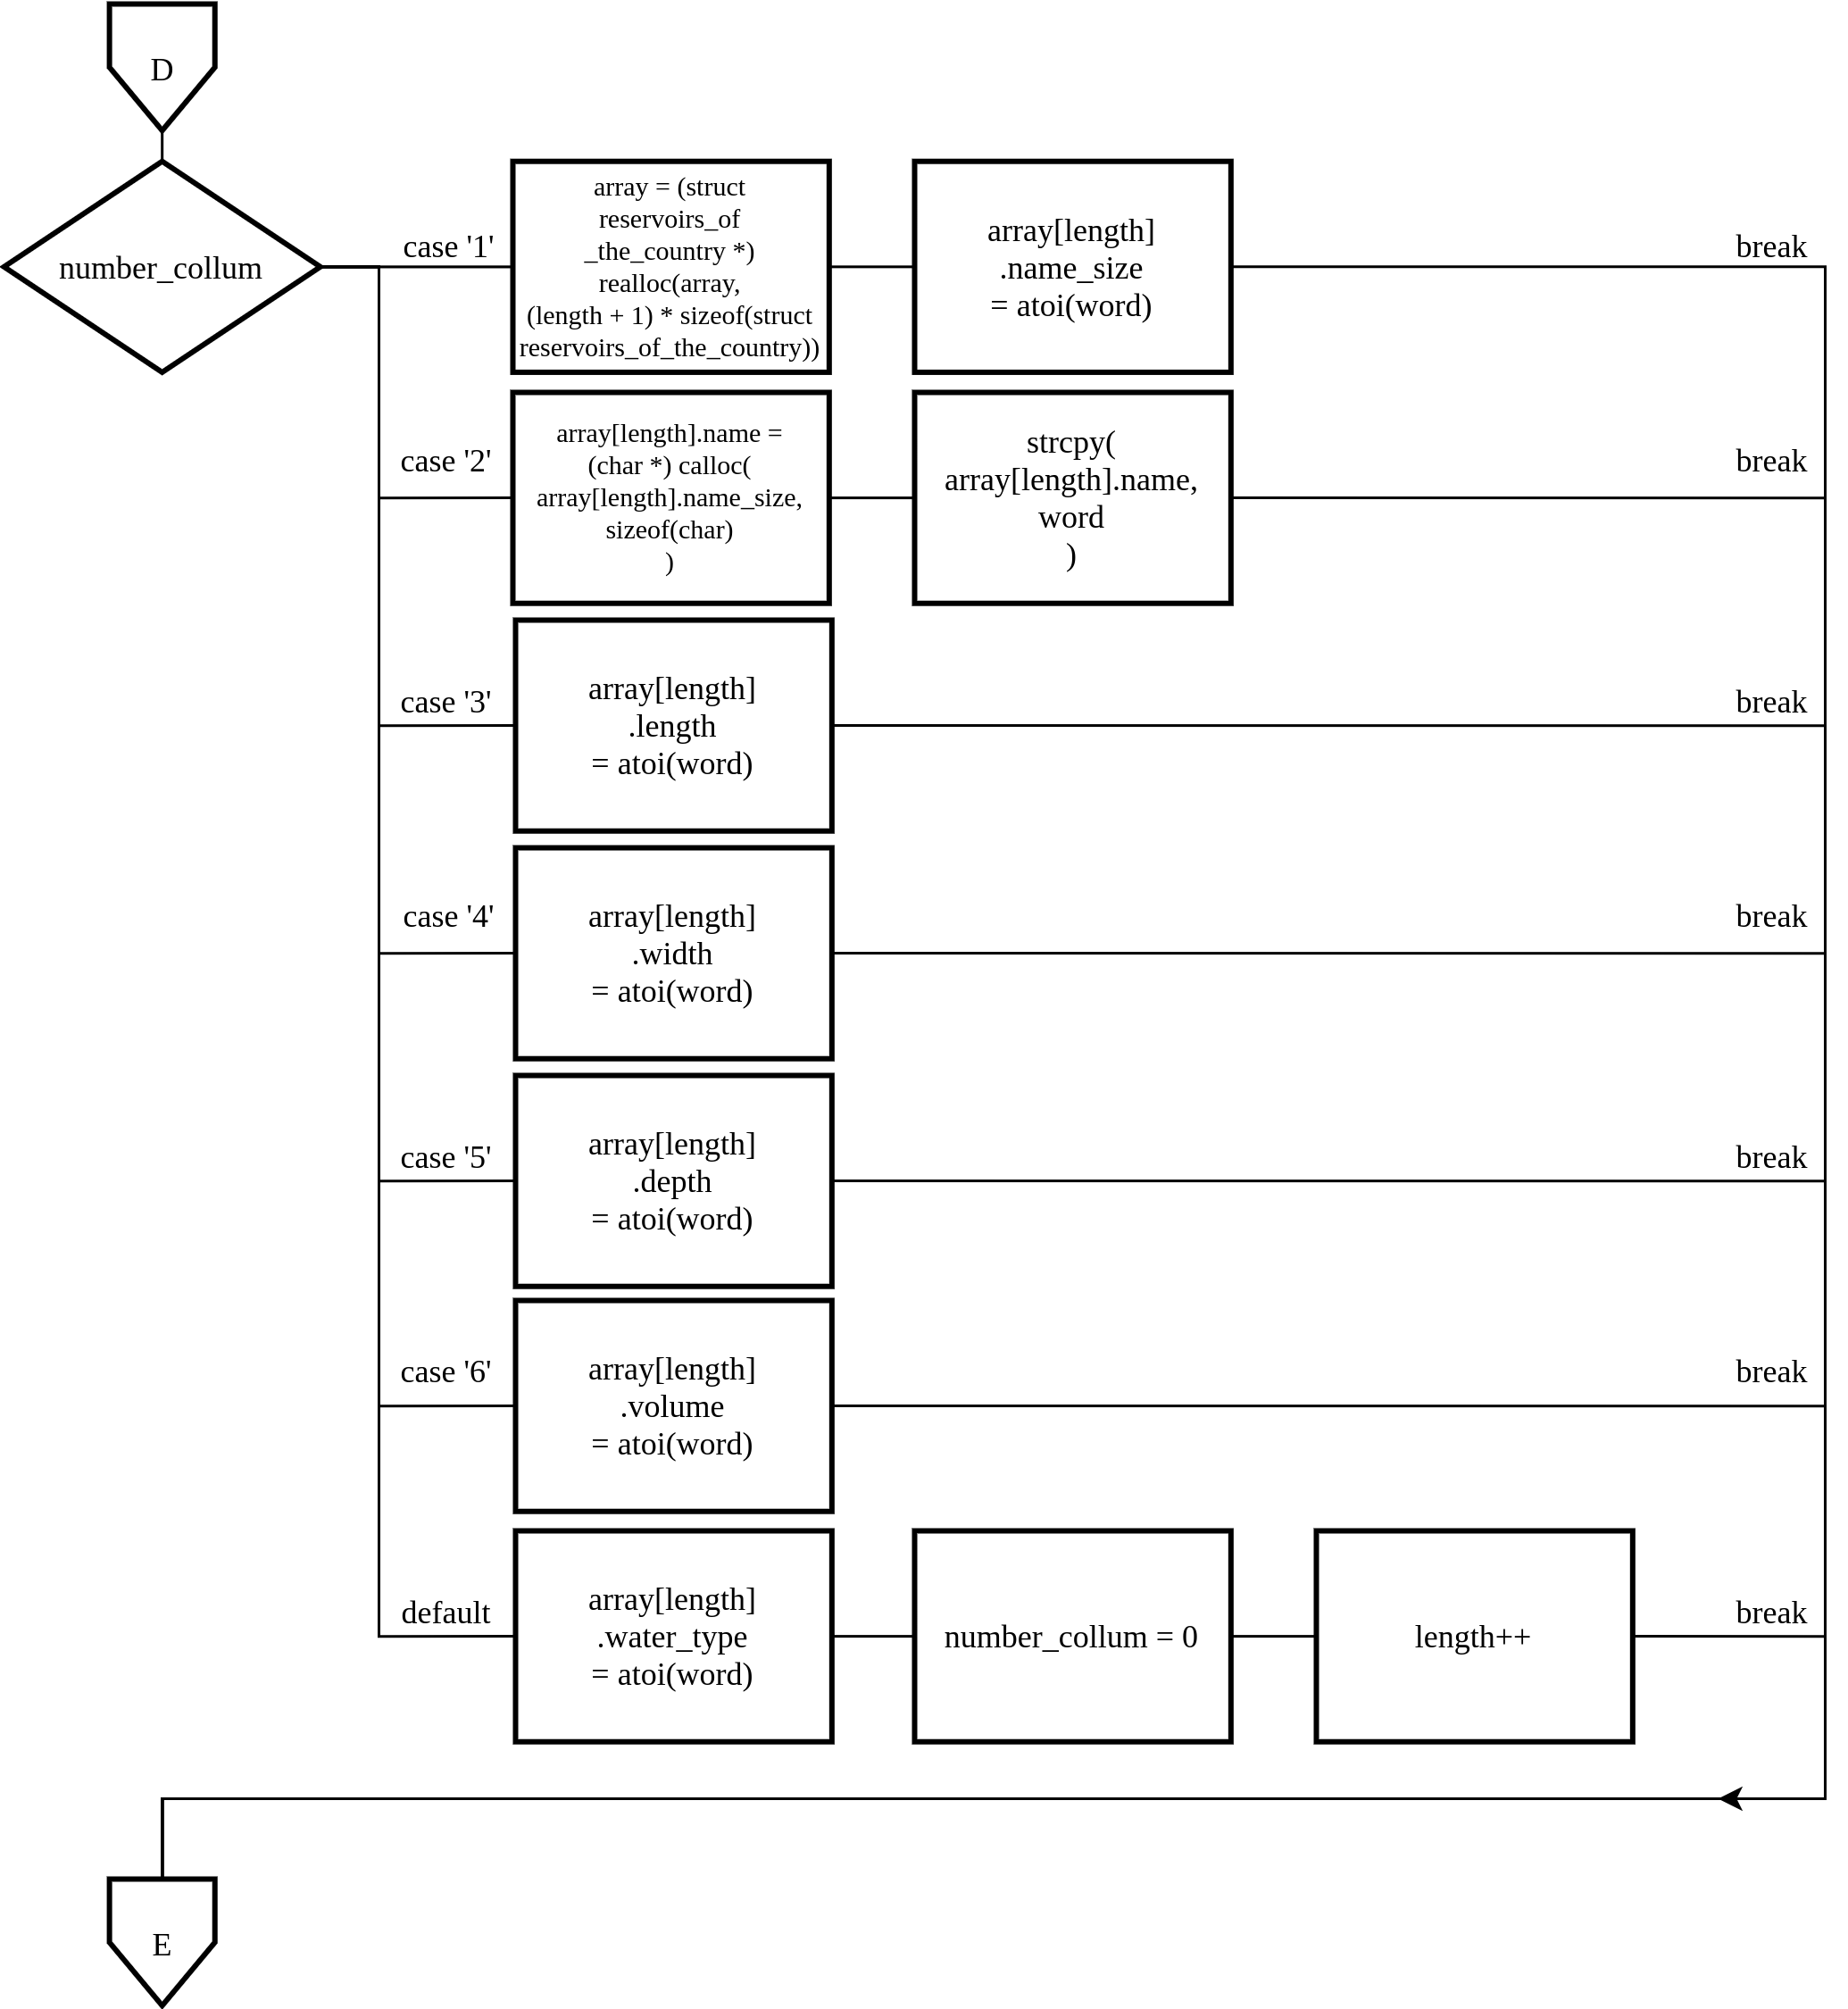
\includegraphics[width=16cm]{../src/app/menu/open_file/open_file-Page-2.png}
    }
    \caption{open\_file() часть 2}
\end{figure}

% = = =

\newpage
\section{Добавление элементов}

% = = =

%menu\_add\_element()
% = = =

%input\_depth()

% = = =

%input\_length()

% = = =

%input\_name()

% = = =

%input\_type()

% = = =

%input\_volume()

% = = =

%input\_ALL\_fields()

% = = =

%add\_element\_before\_element()

% = = =

%replace\_element()

% = = =

%add\_element\_on\_position()

% = = =

%add\_element\_after\_element()

% = = =

%add\_element\_on\_end()

% = = =

\newpage
\section{Вывод данных}

% = = =

%out\_data()

% = = =

%print\_sep()

% = = =

%print\_line()

% = = =

%write\_head\_table()

% = = =

%write\_one\_element()

% = = =

%write\_one\_edit\_element()

% = = =

%write\_table\_on\_range()

% = = =

%out\_average\_values\_in\_line()

% = = =

%out\_max\_values\_in\_line()

% = = =

%out\_min\_values\_in\_line()

% = = =

\newpage
\section{Сохранение файла}

% = = =

\begin{figure}[H]
    \center{
        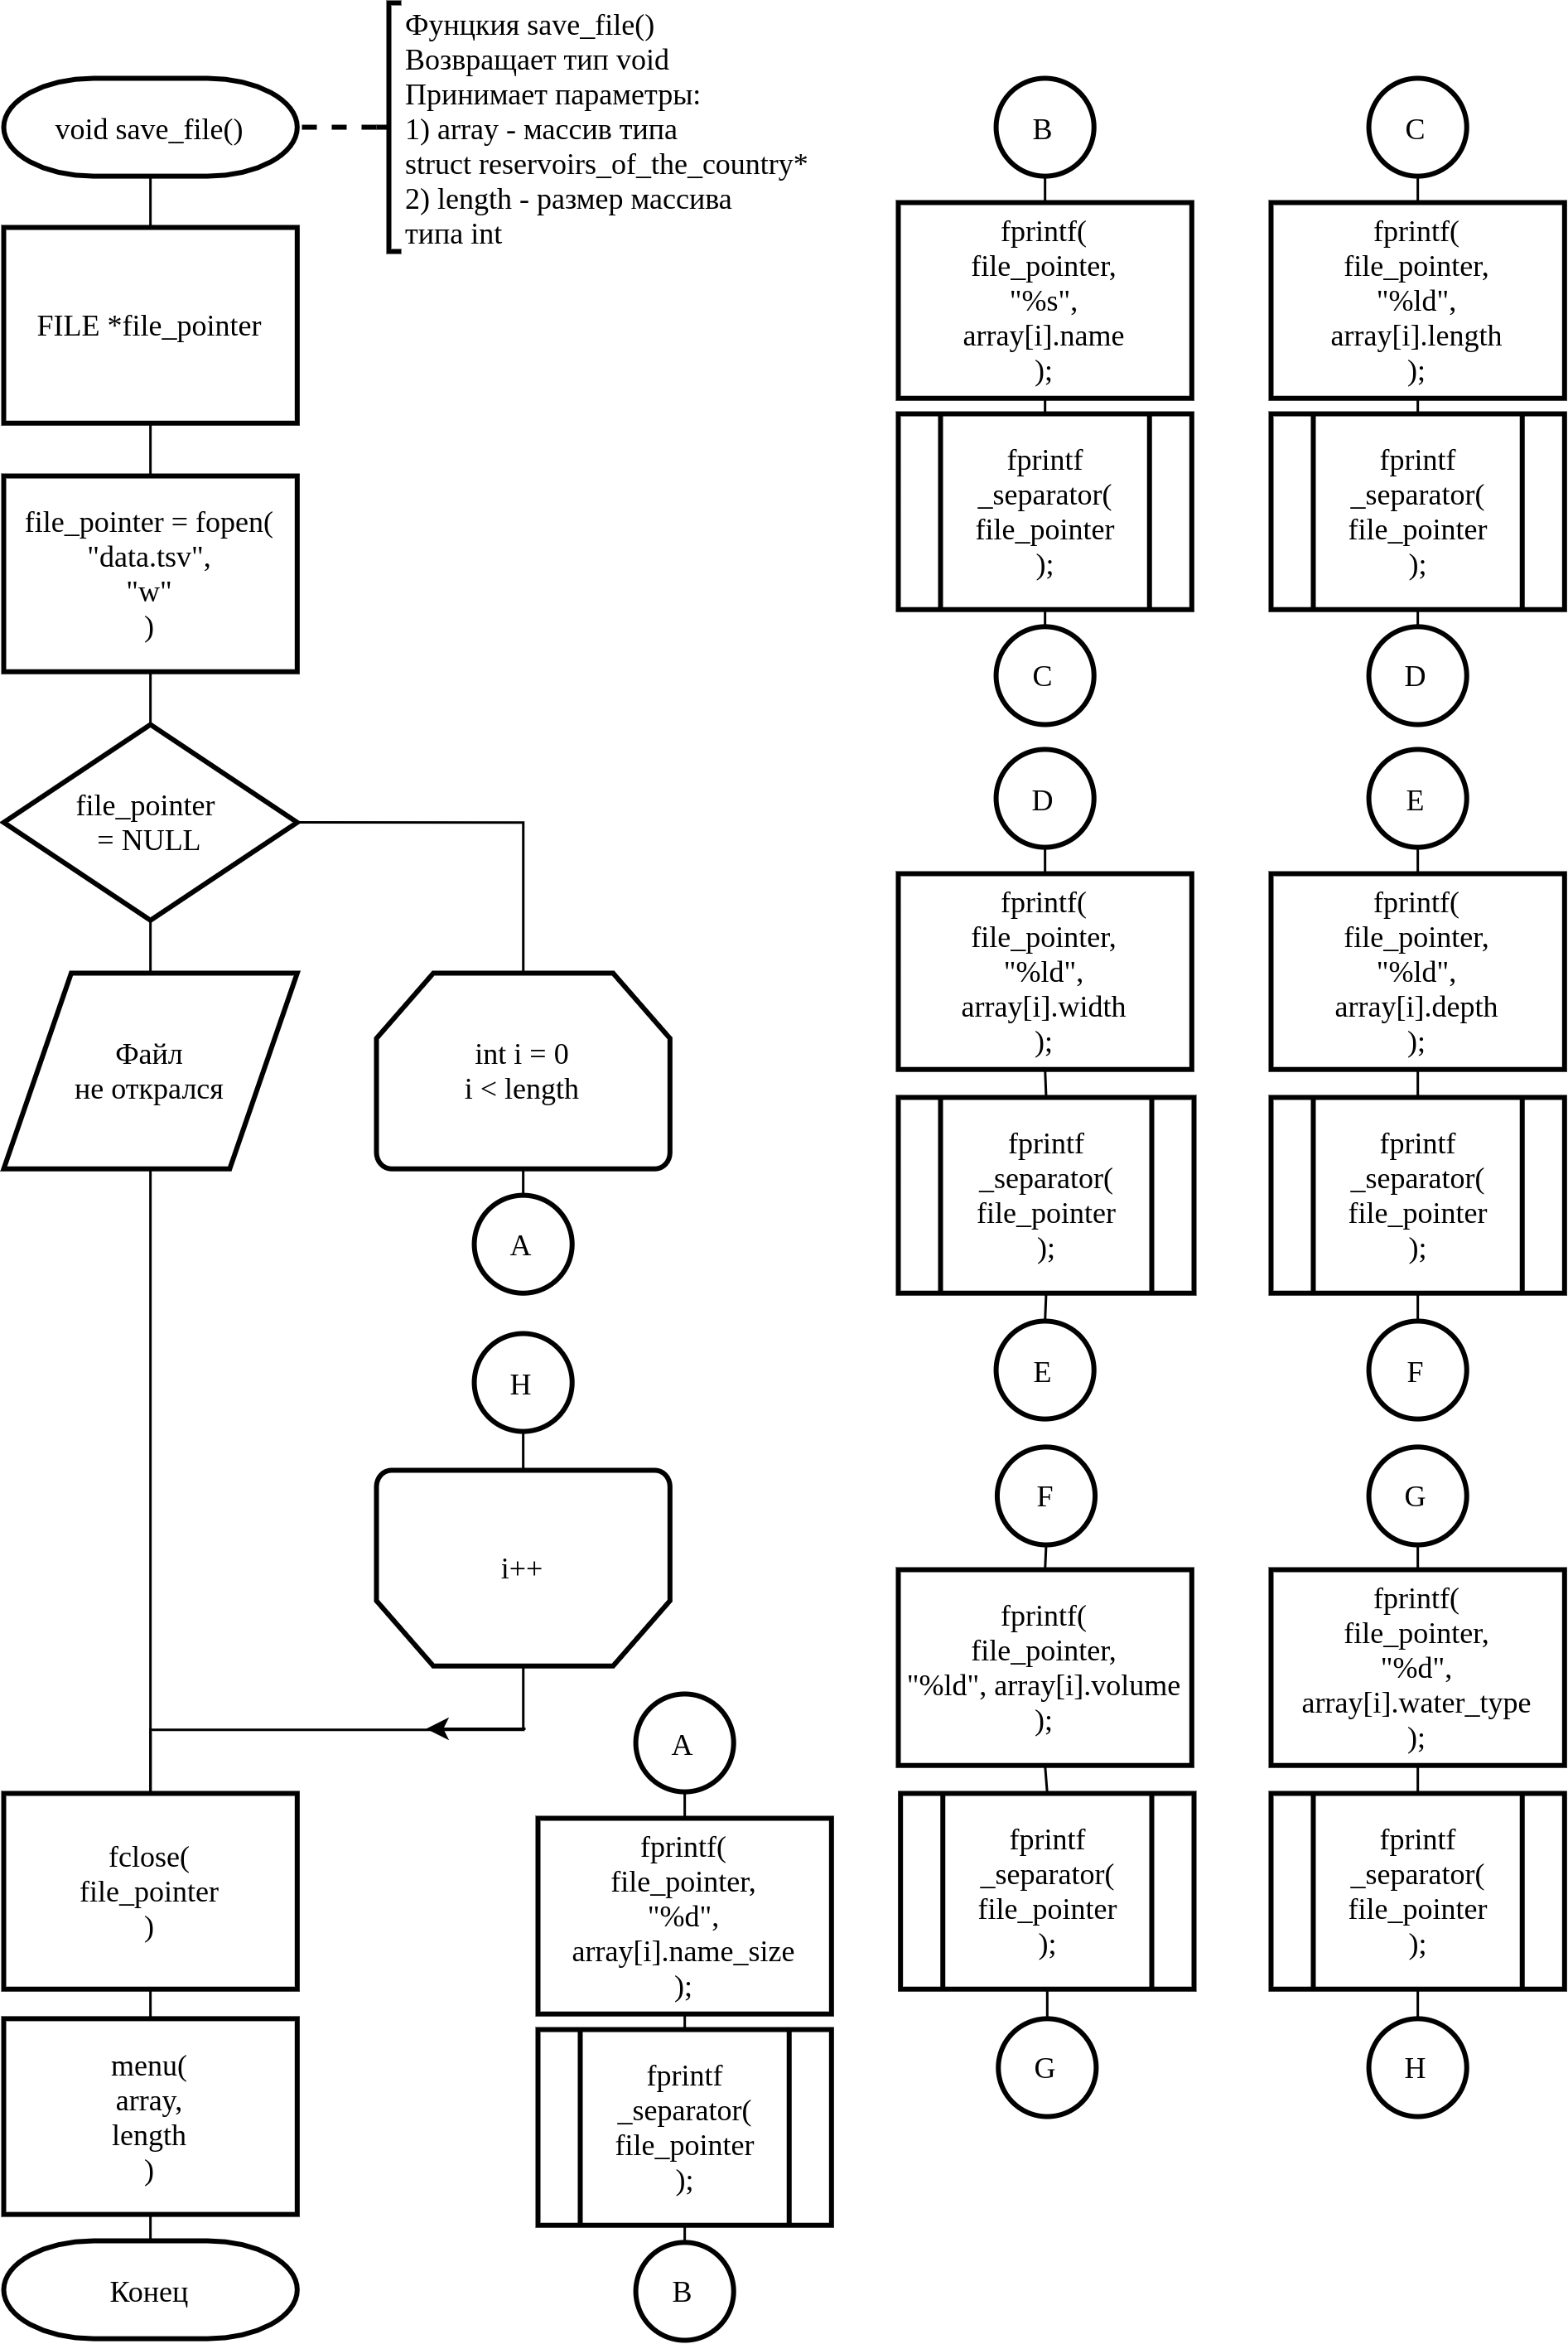
\includegraphics[]{../src/app/menu/save_file/save_file.png}
    }
    \caption{save\_file()}
\end{figure}

% = = =

\newpage
\section{Корректировать поле}

% = = =

\begin{figure}[H]
    \center{
        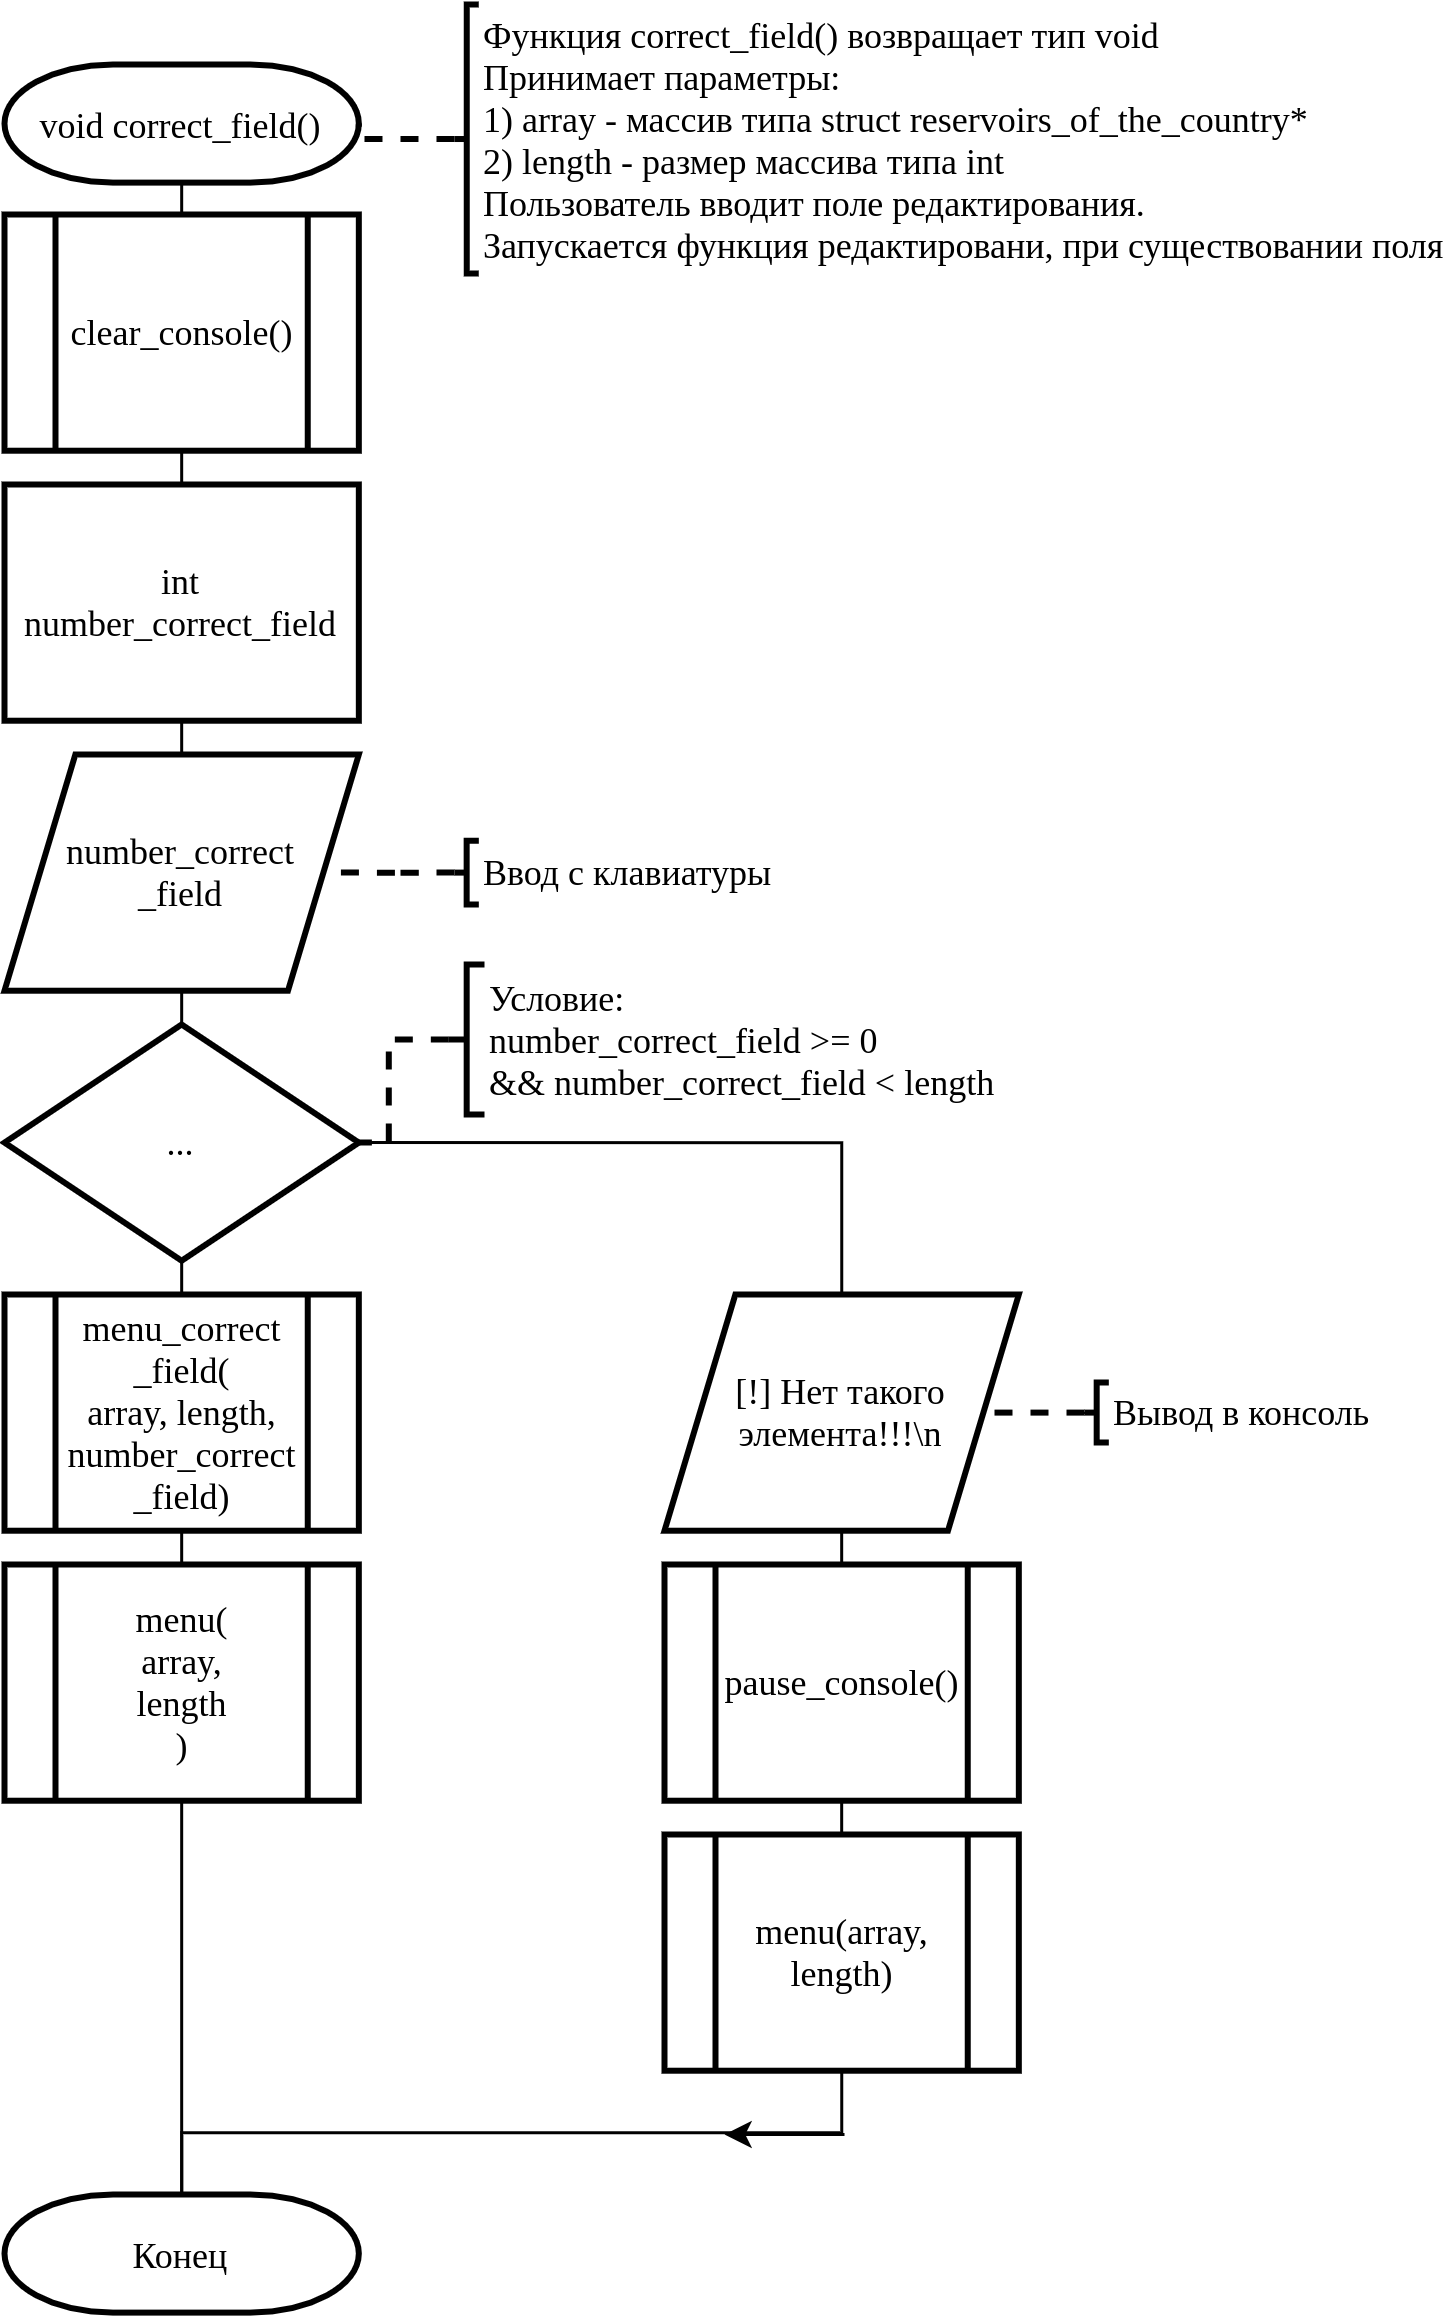
\includegraphics[]{../src/app/menu/correct_field/correct_field.png}
    }
    \caption{correct\_field()}
\end{figure}

% = = =

\begin{figure}[H]
    \center{
        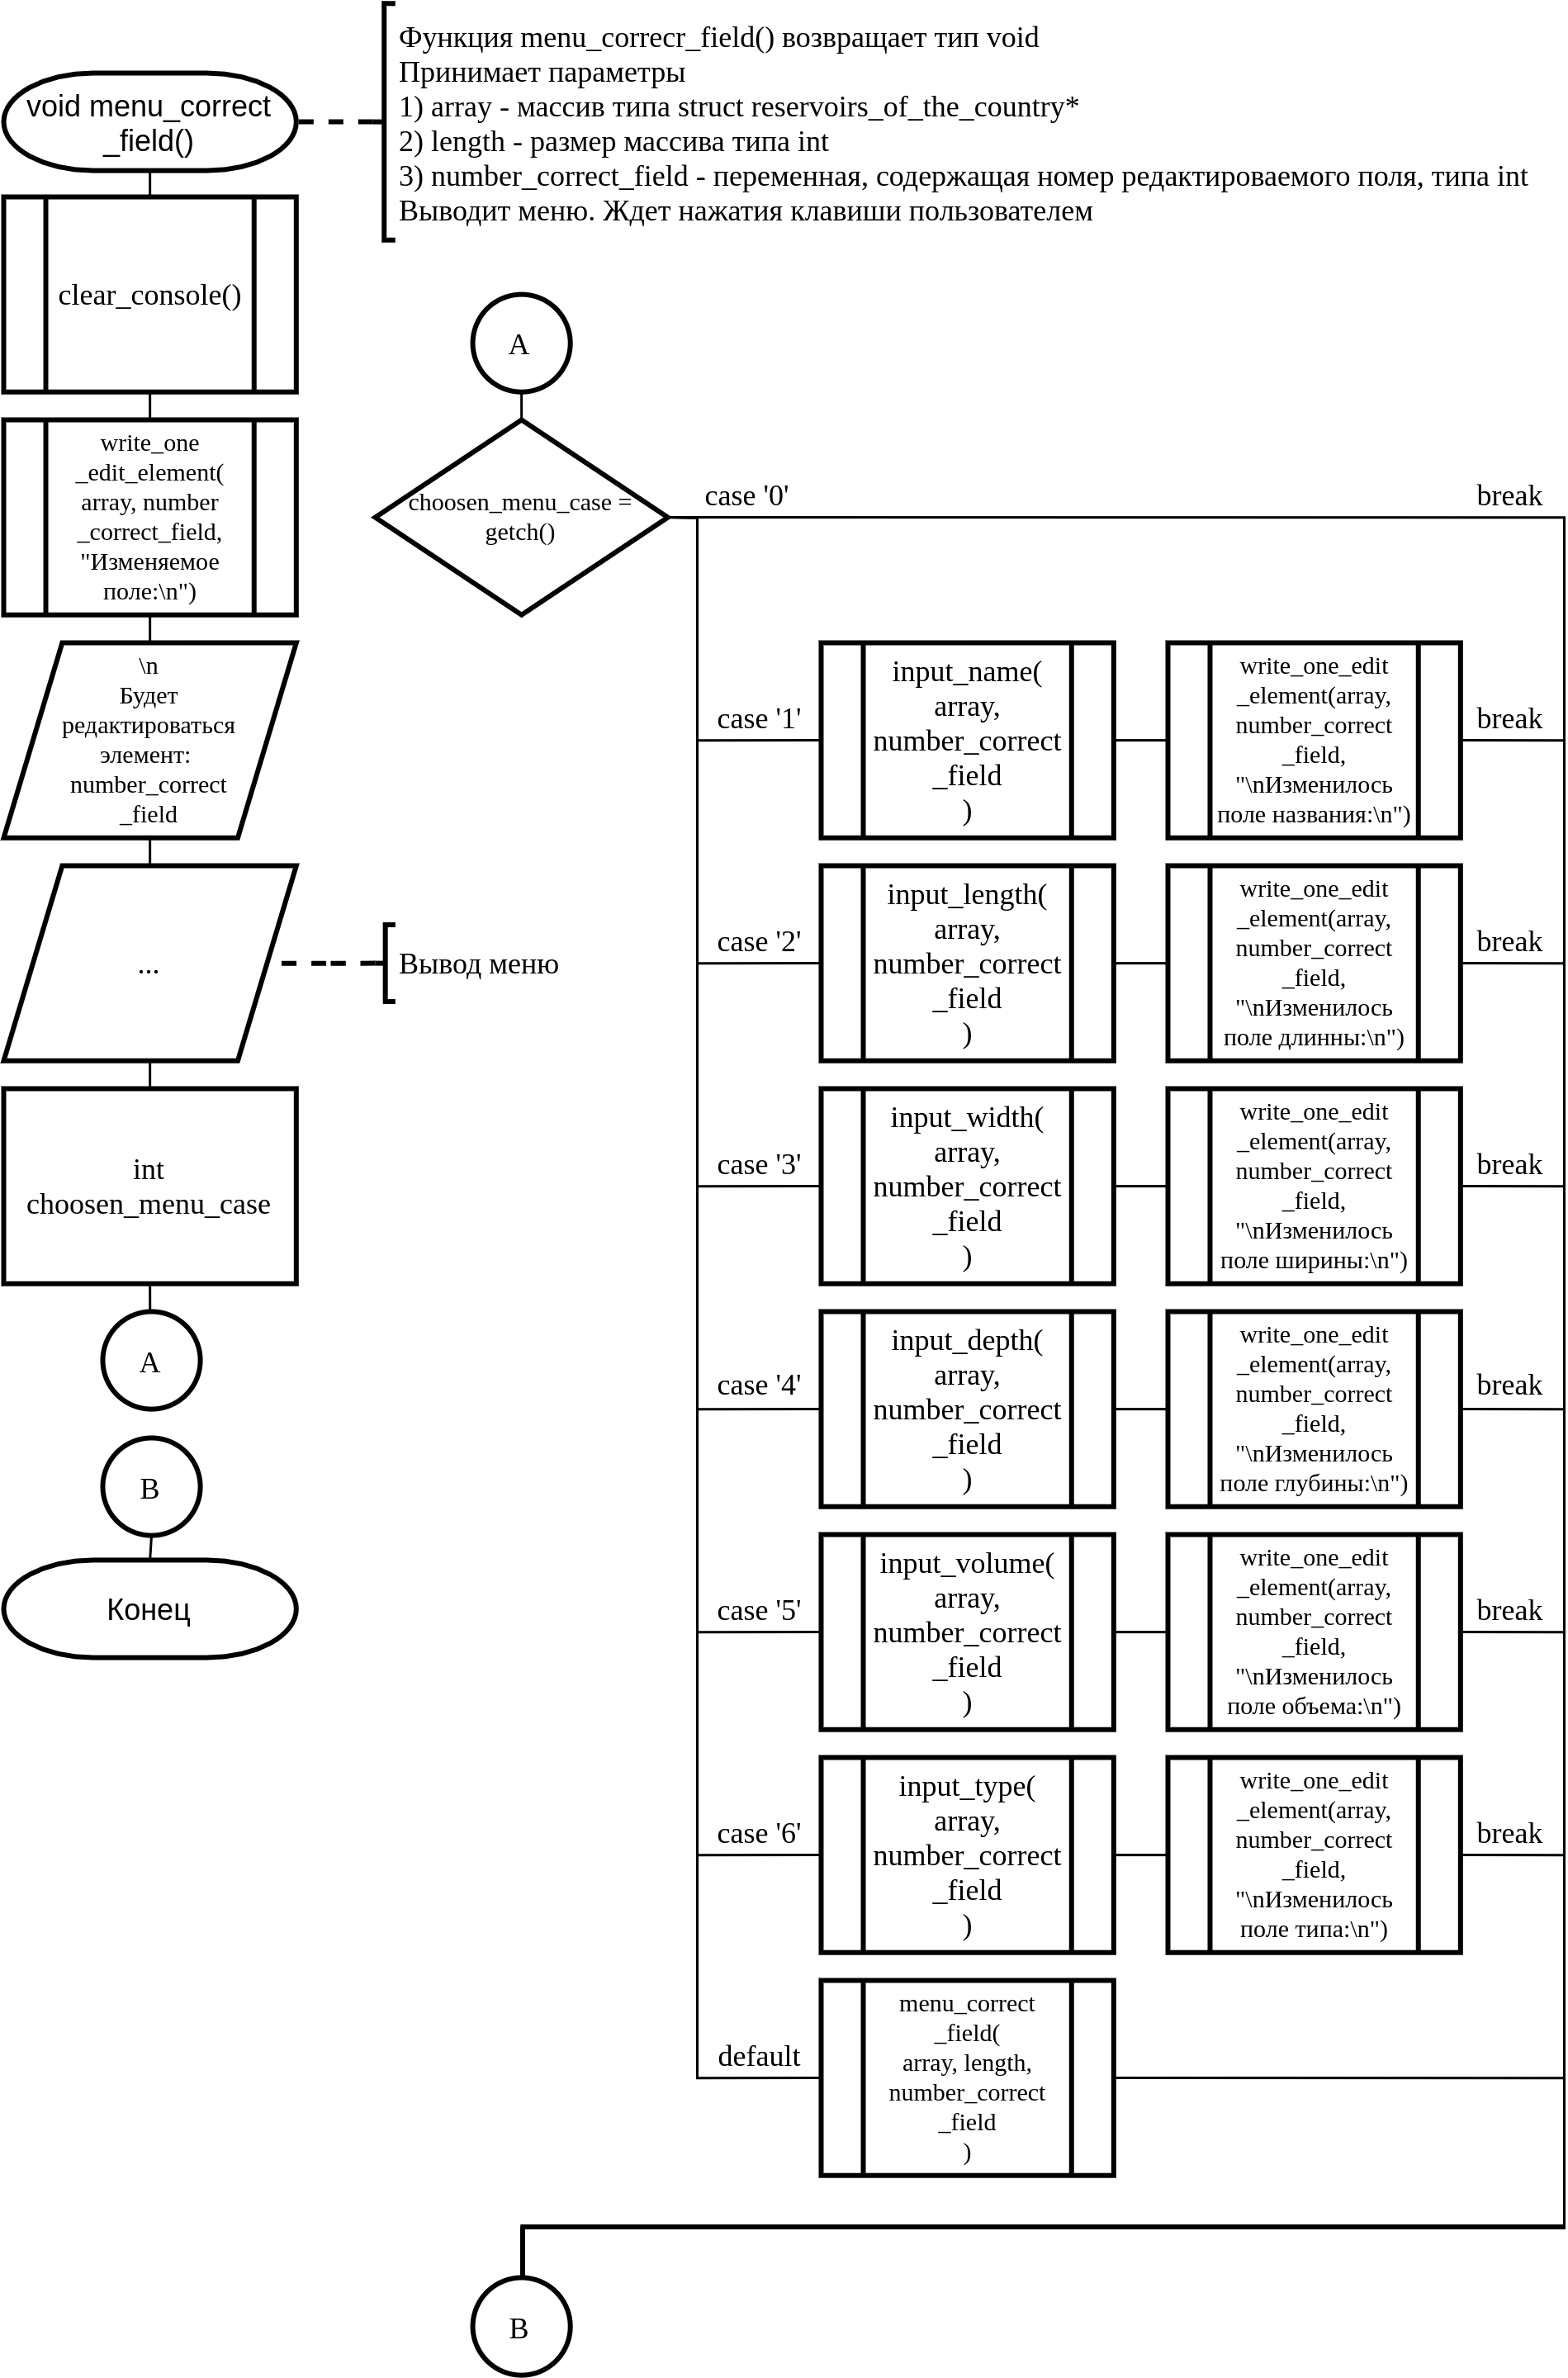
\includegraphics[]{../src/app/menu/correct_field/menu_correct_field/menu_correct_field.png}
    }
    \caption{menu\_correct\_field()}
\end{figure}

% = = =

\newpage
\section{Удаление элементов}

% = = =

%menu\_del\_data()

% = = =

%del\_one\_element()

% = = =

%del\_data\_from()

% = = =

%menu\_del\_less\_value\_field()

% = = =

%del\_if\_less\_depth()

% = = =

%del\_if\_less\_length()

% = = =

%del\_if\_less\_volume()

% = = =

%del\_if\_less\_width()

% = = =

%menu\_del\_more\_value\_field()

% = = =

%del\_if\_more\_depth()

% = = =

%del\_if\_more\_length()

% = = =

%del\_if\_more\_volume()

% = = =

%el\_if\_more\_width()

% = = =

\newpage
\section{Сортировка}

% = = =

\begin{figure}[H]
    \center{
        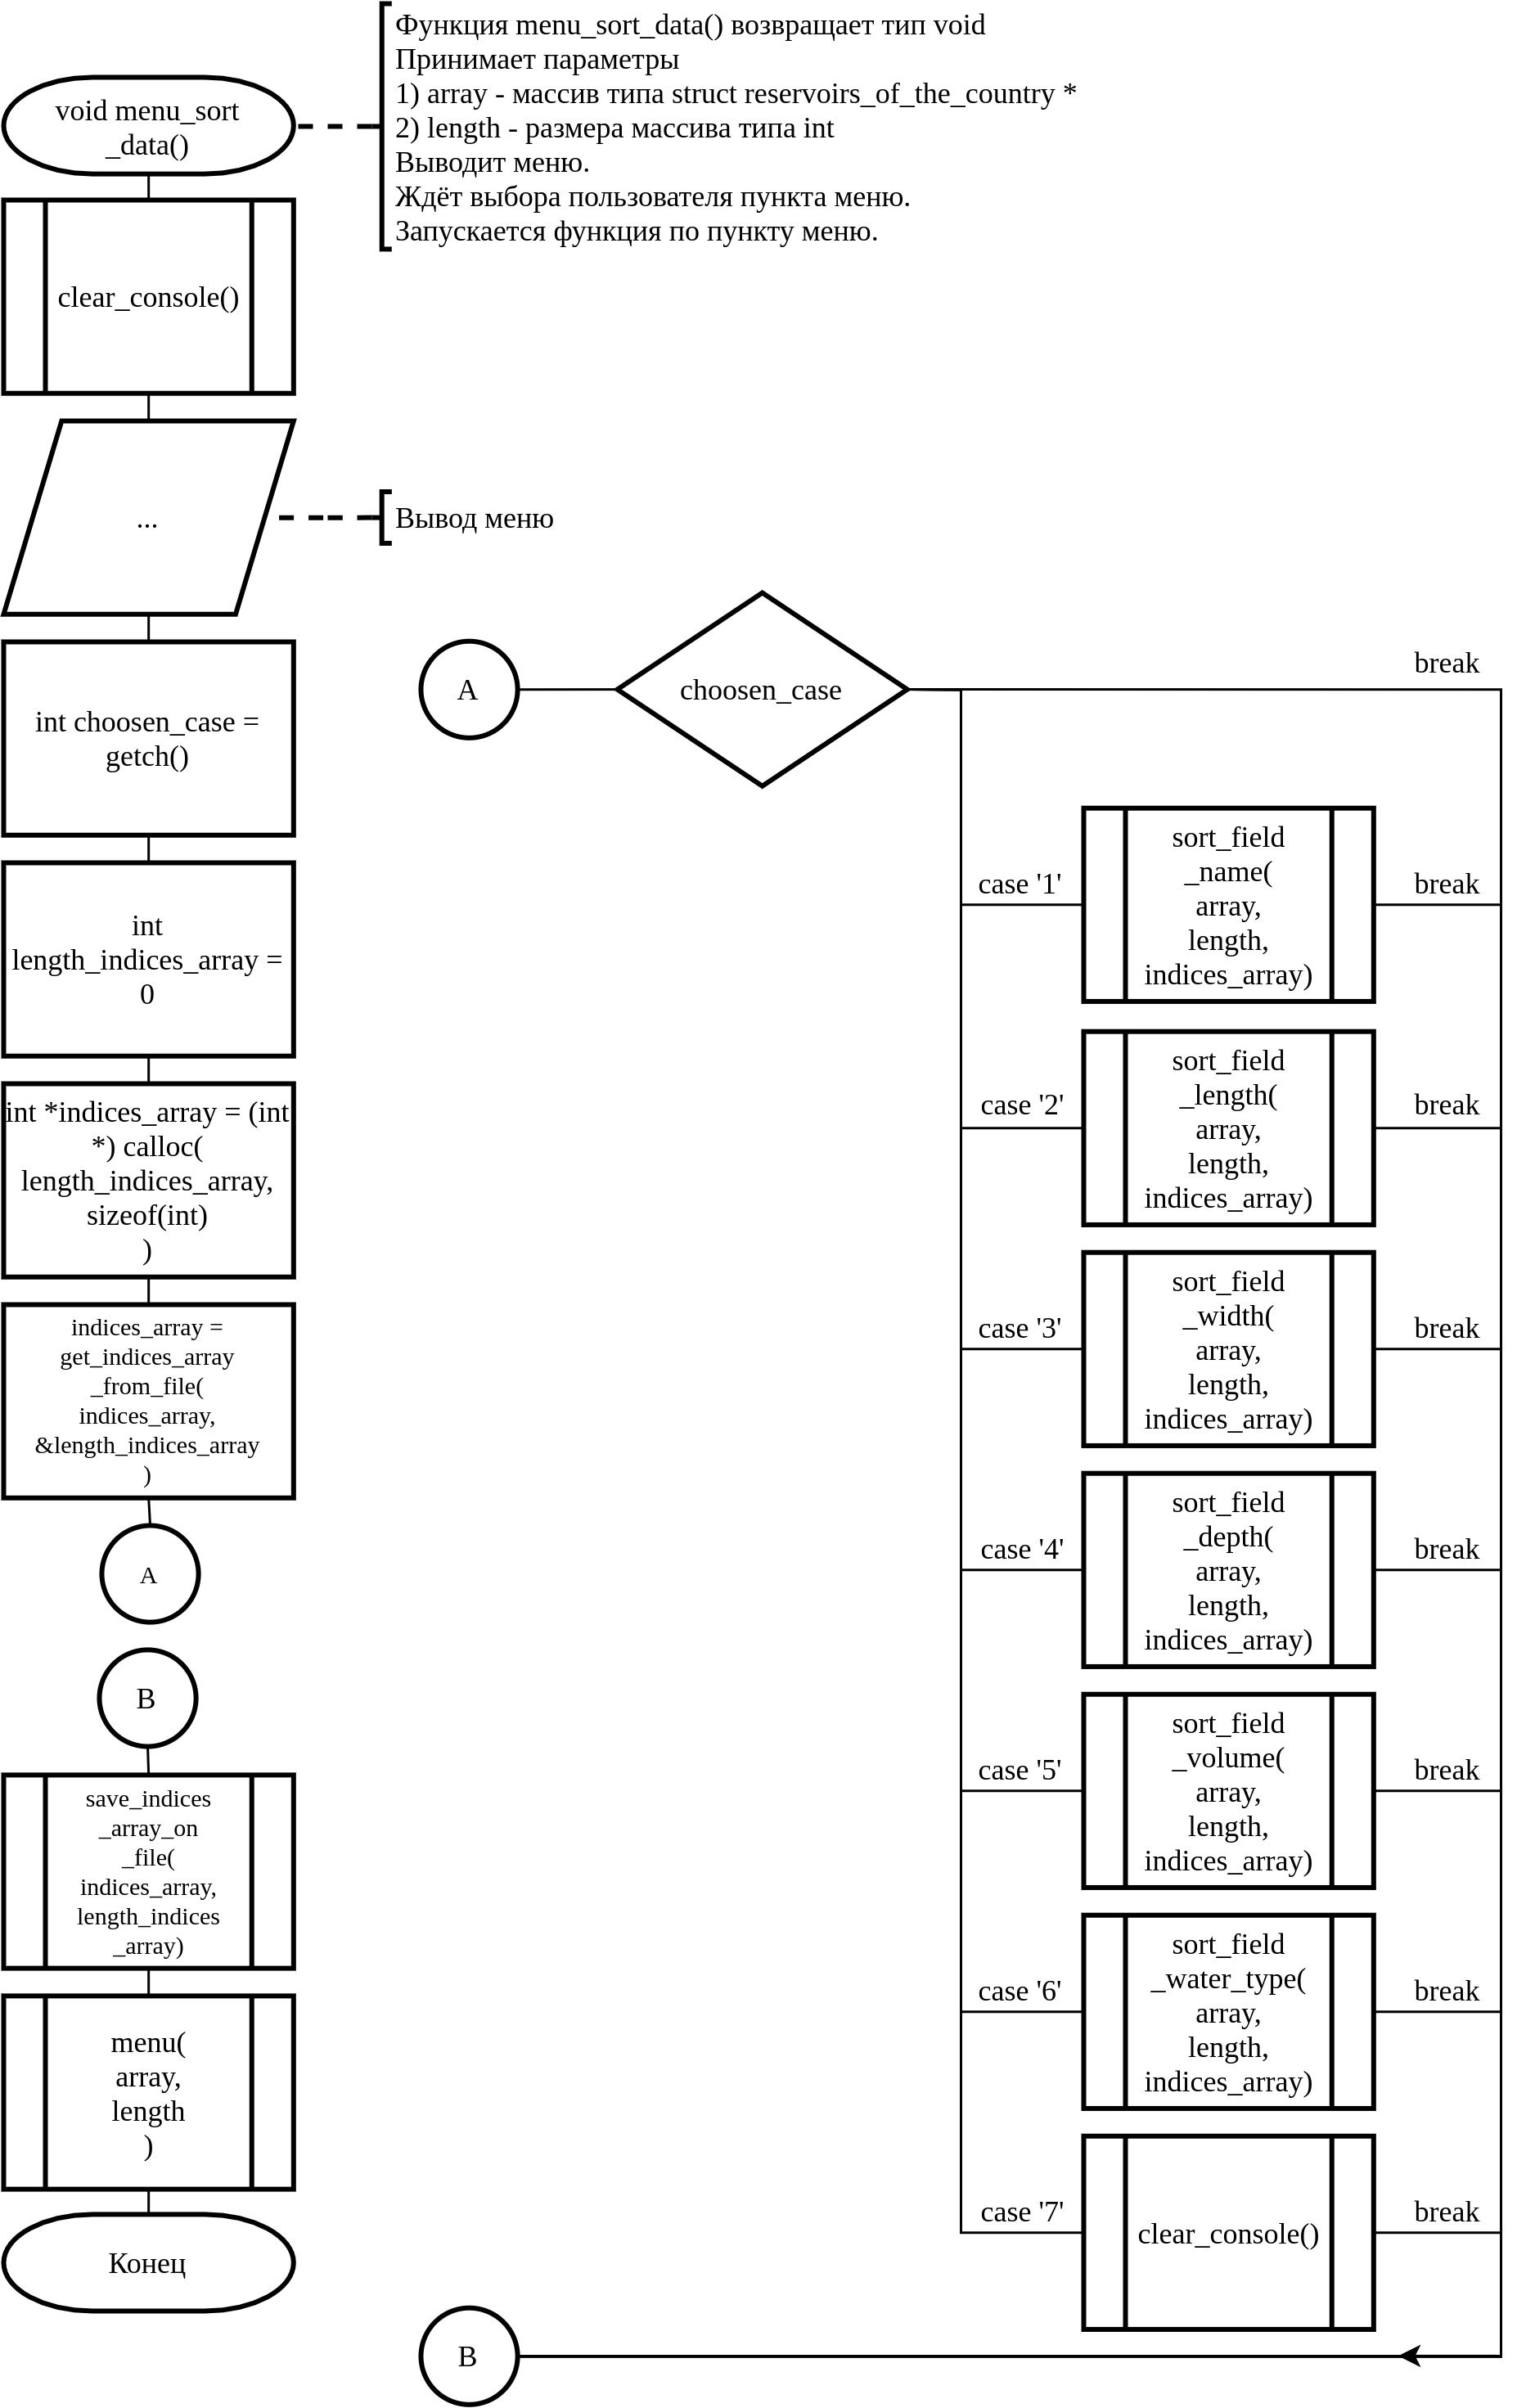
\includegraphics[height=24cm]{../src/app/menu/menu_sort_data/menu_sort_data.png}
    }
    \caption{menu\_sort\_data()}
\end{figure}

% = = =

\begin{figure}[H]
    \center{
        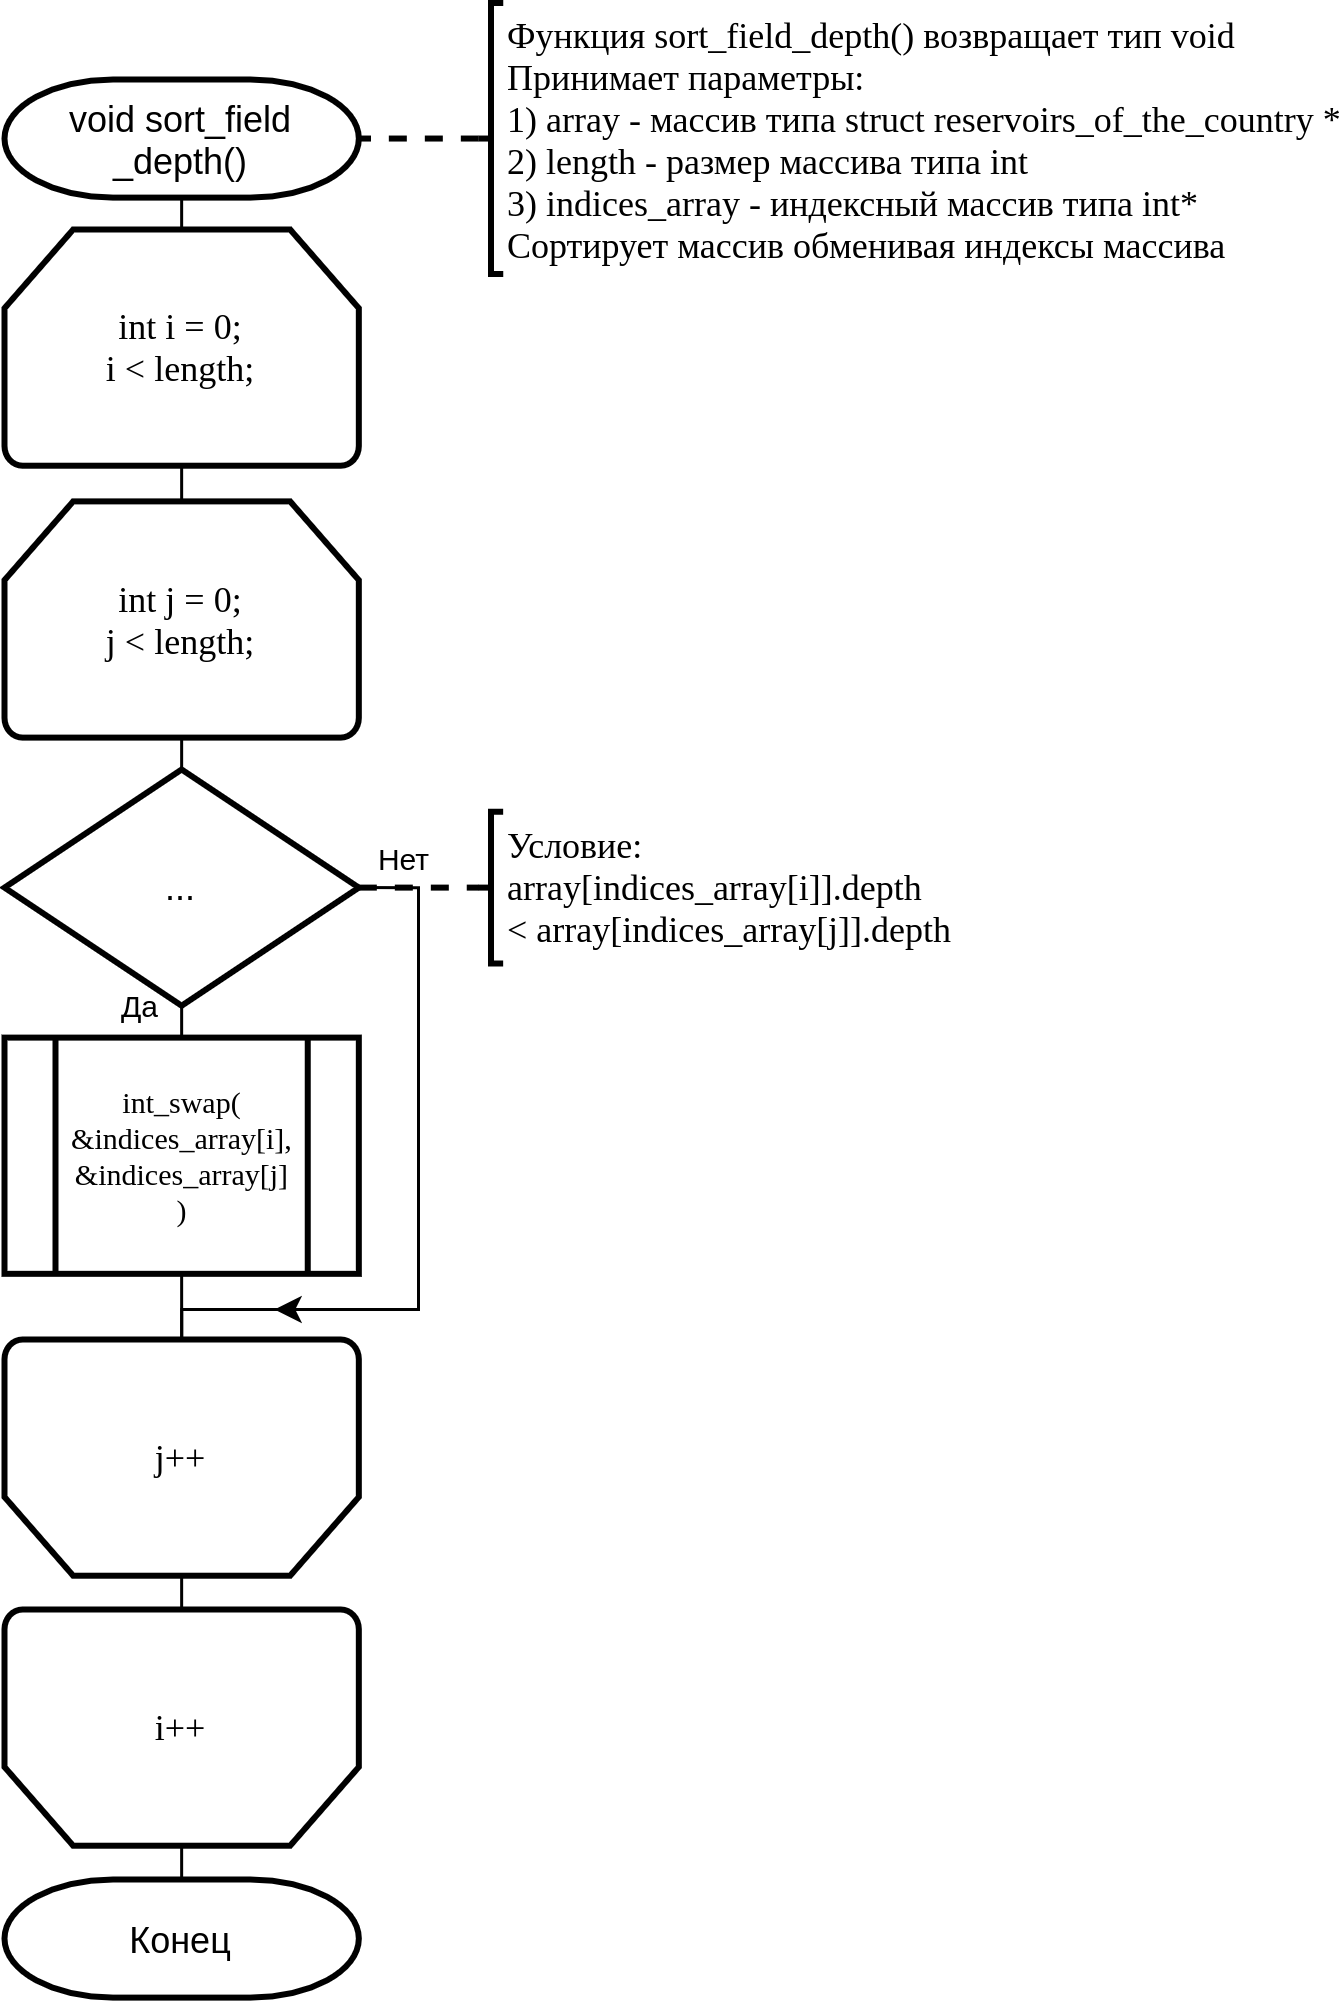
\includegraphics[]{../src/app/menu/menu_sort_data/sort_field_depth/sort_field_depth.png}
    }
    \caption{sort\_field\_depth()}
\end{figure}

% = = =

\begin{figure}[H]
    \center{
        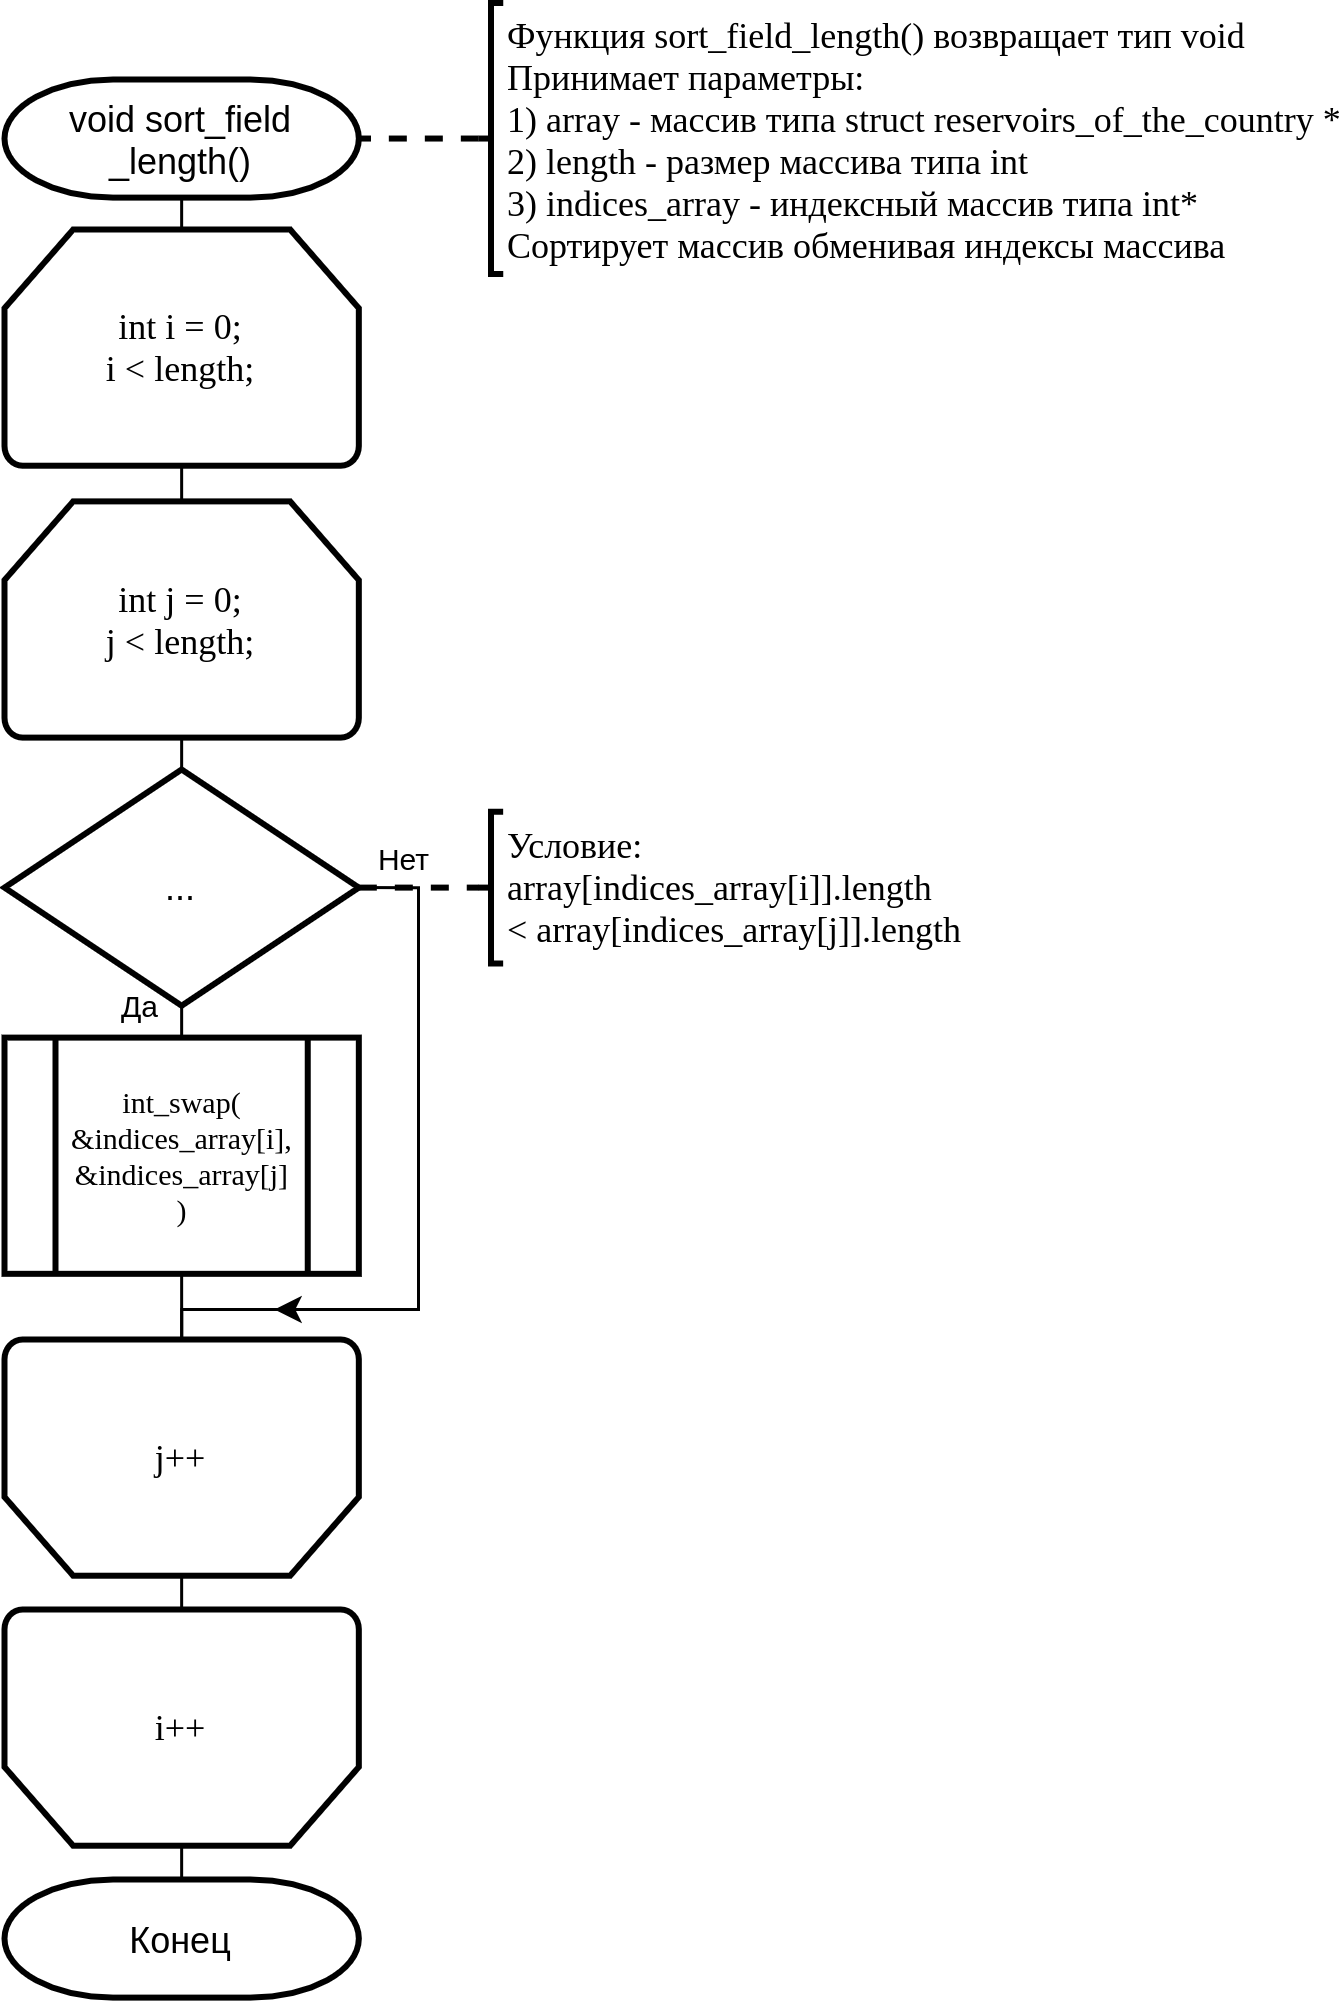
\includegraphics[]{../src/app/menu/menu_sort_data/sort_field_length/sort_field_length.png}
    }
    \caption{sort\_field\_length()}
\end{figure}

% = = =

\begin{figure}[H]
    \center{
        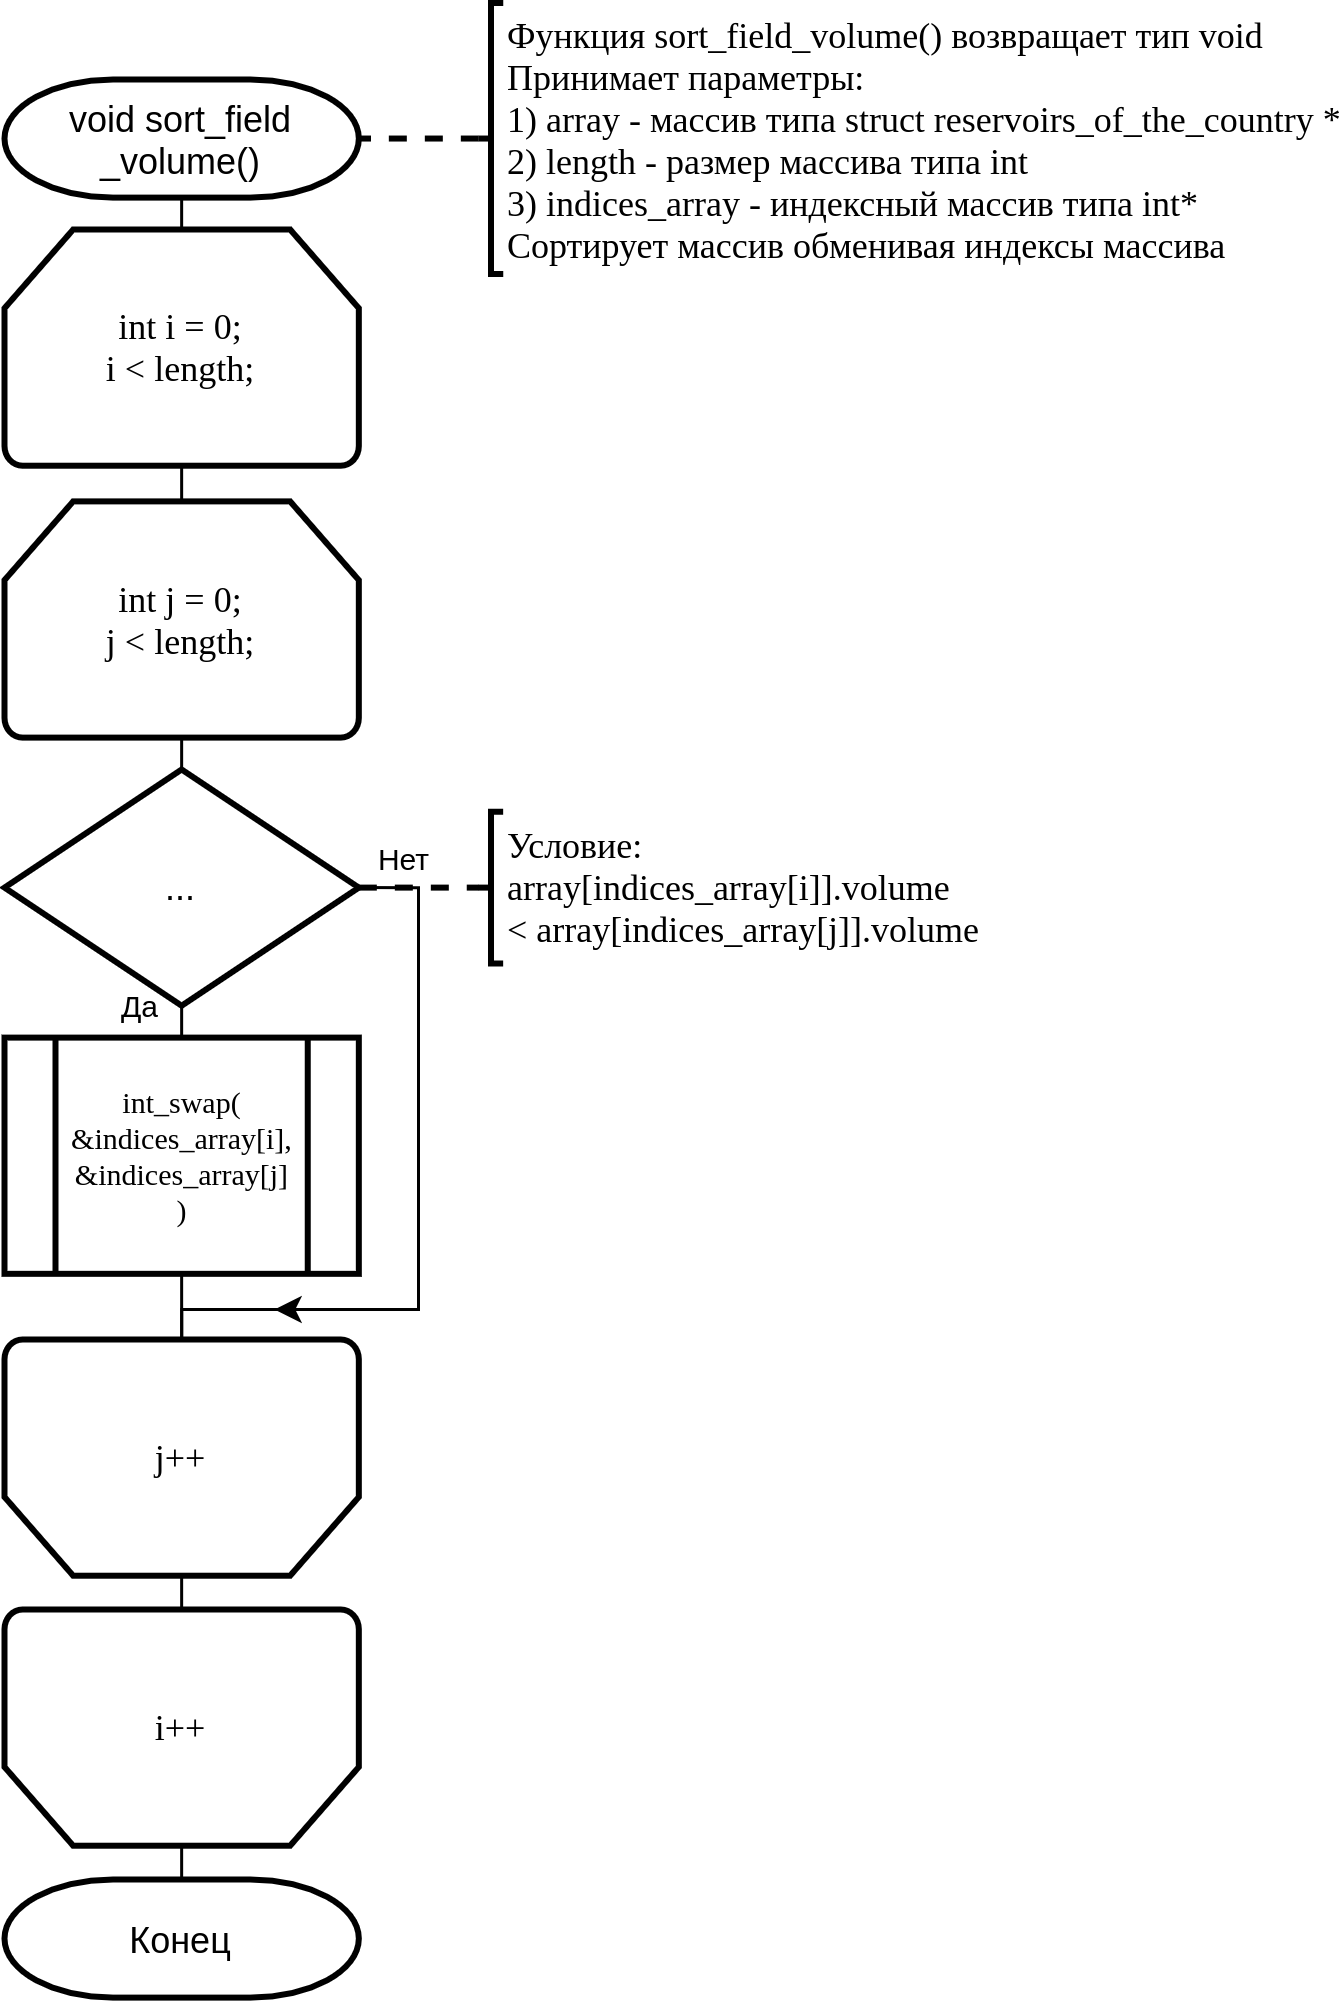
\includegraphics[]{../src/app/menu/menu_sort_data/sort_field_volume/sort_field_volume.png}
    }
    \caption{sort\_field\_volume()}
\end{figure}

% = = =

\begin{figure}[H]
    \center{
        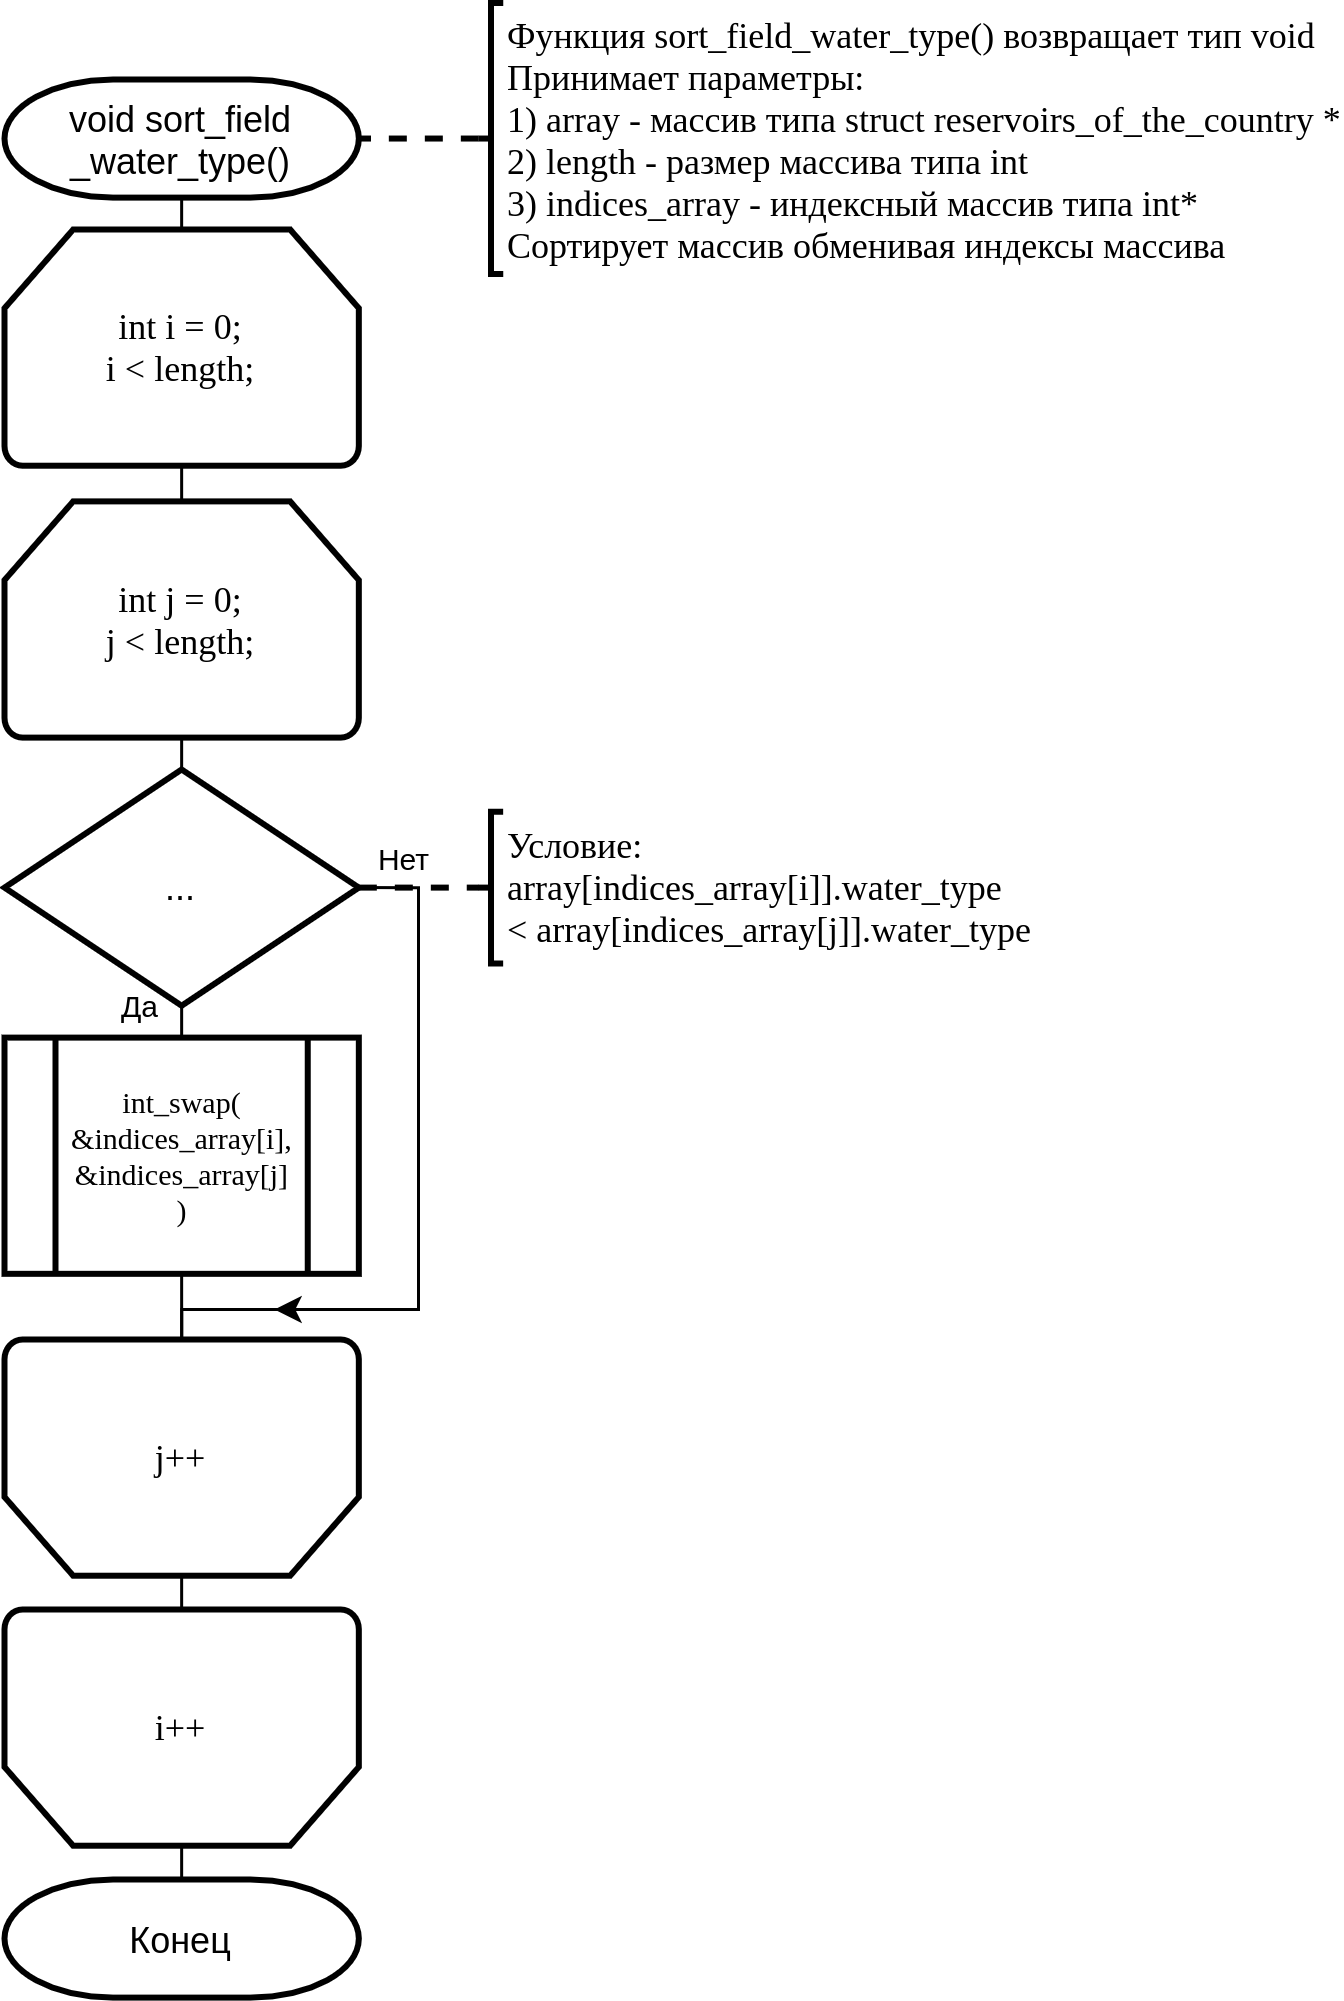
\includegraphics[]{../src/app/menu/menu_sort_data/sort_field_water_type/sort_field_water_type.png}
    }
    \caption{sort\_field\_water\_type()}
\end{figure}

% = = =

\begin{figure}[H]
    \center{
        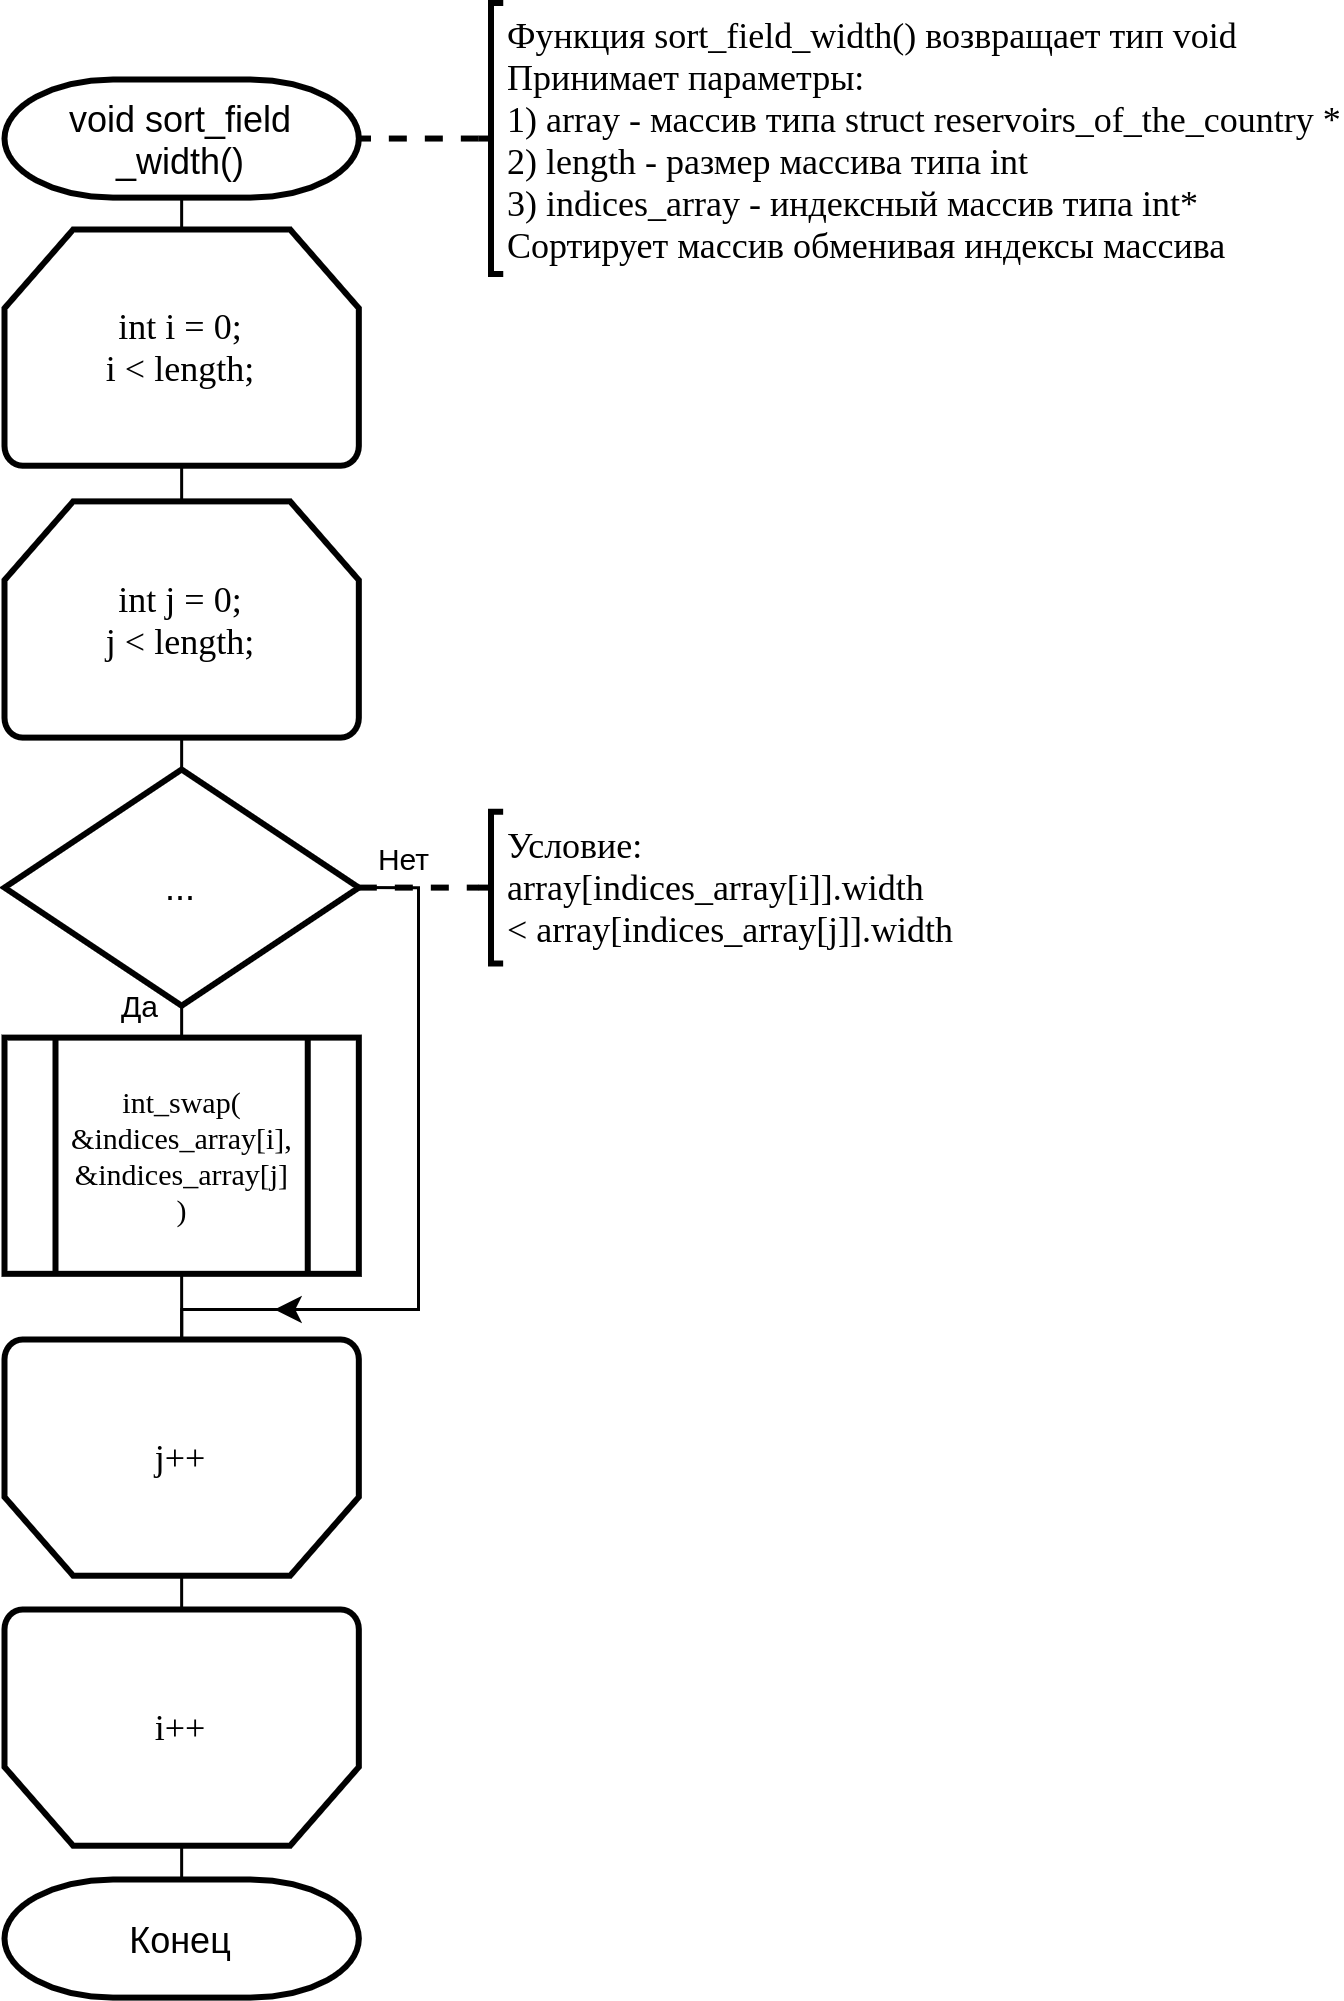
\includegraphics[]{../src/app/menu/menu_sort_data/sort_field_width/sort_field_width.png}
    }
    \caption{sort\_field\_width()}
\end{figure}

% = = =

\newpage
\section{Поиск min/max в диапазоне}

% = = =

\begin{figure}[H]
    \center{
        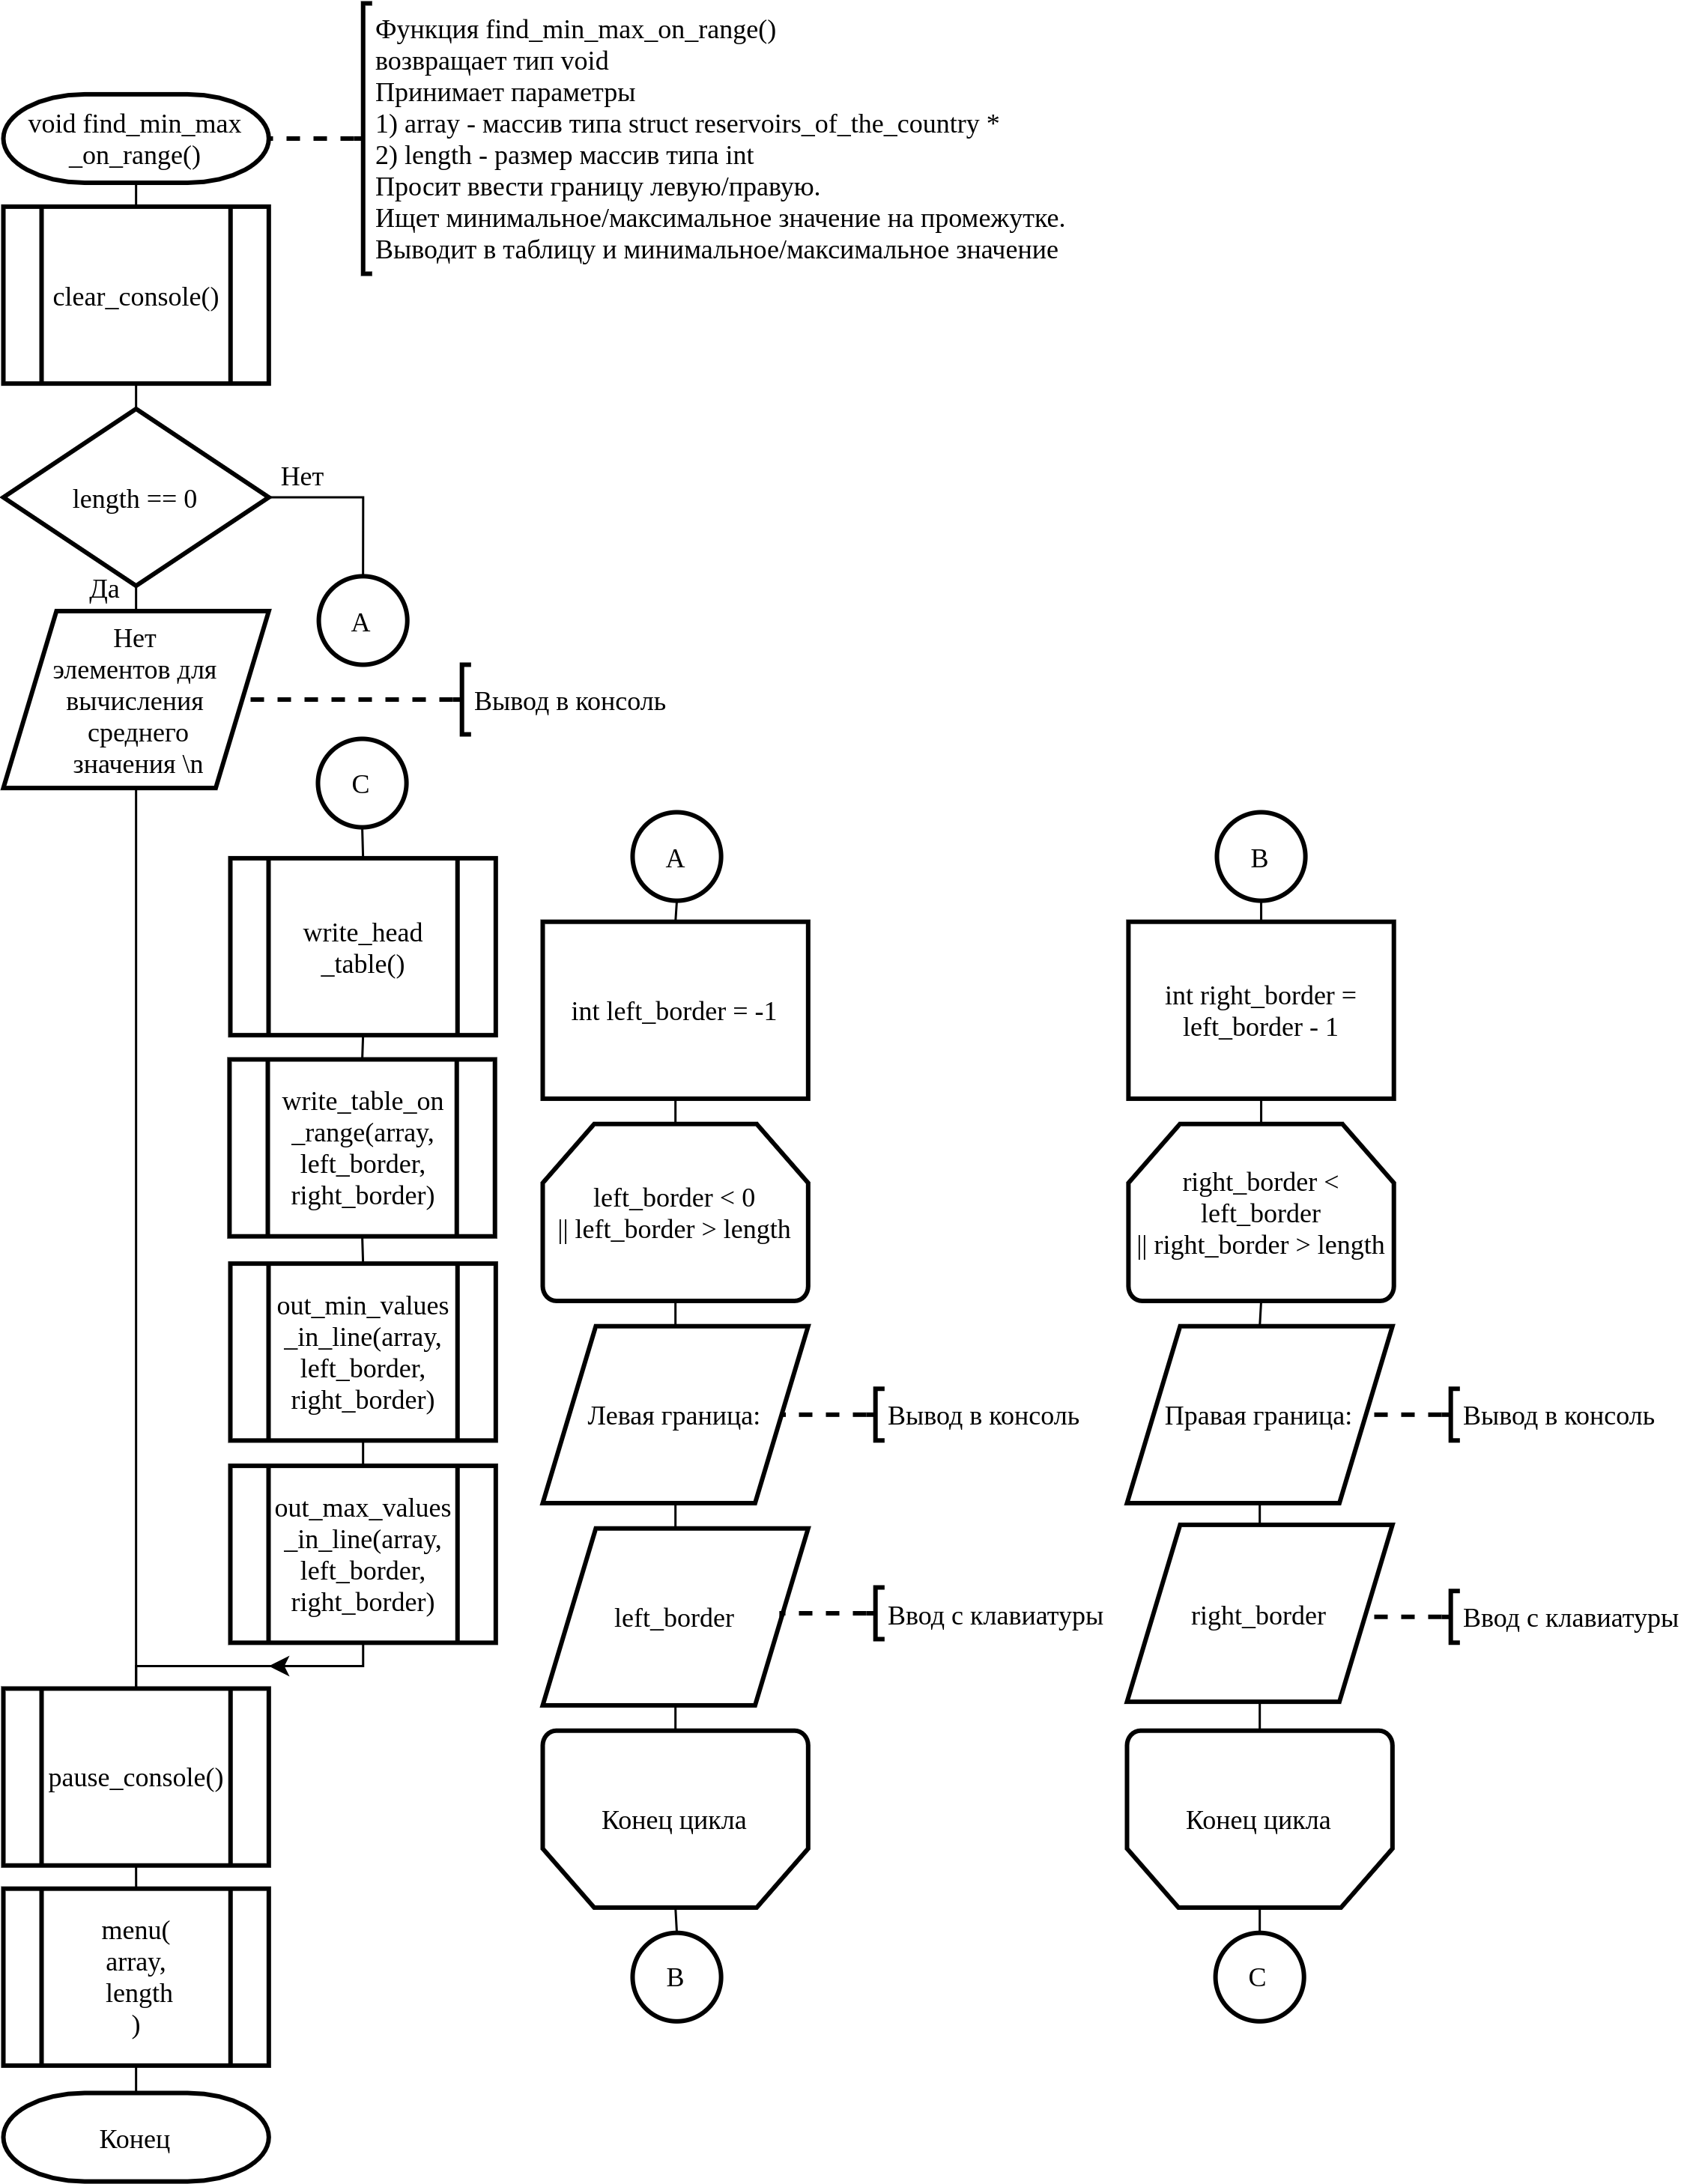
\includegraphics[width=16cm]{../src/app/menu/find_min_max_on_range/find_min_max_on_range.png}
    }
    \caption{find\_min\_max\_on\_range()}
\end{figure}

% = = =

\newpage
\section{Поиск среднего в диапазоне}

% = = =

\begin{figure}[H]
    \center{
        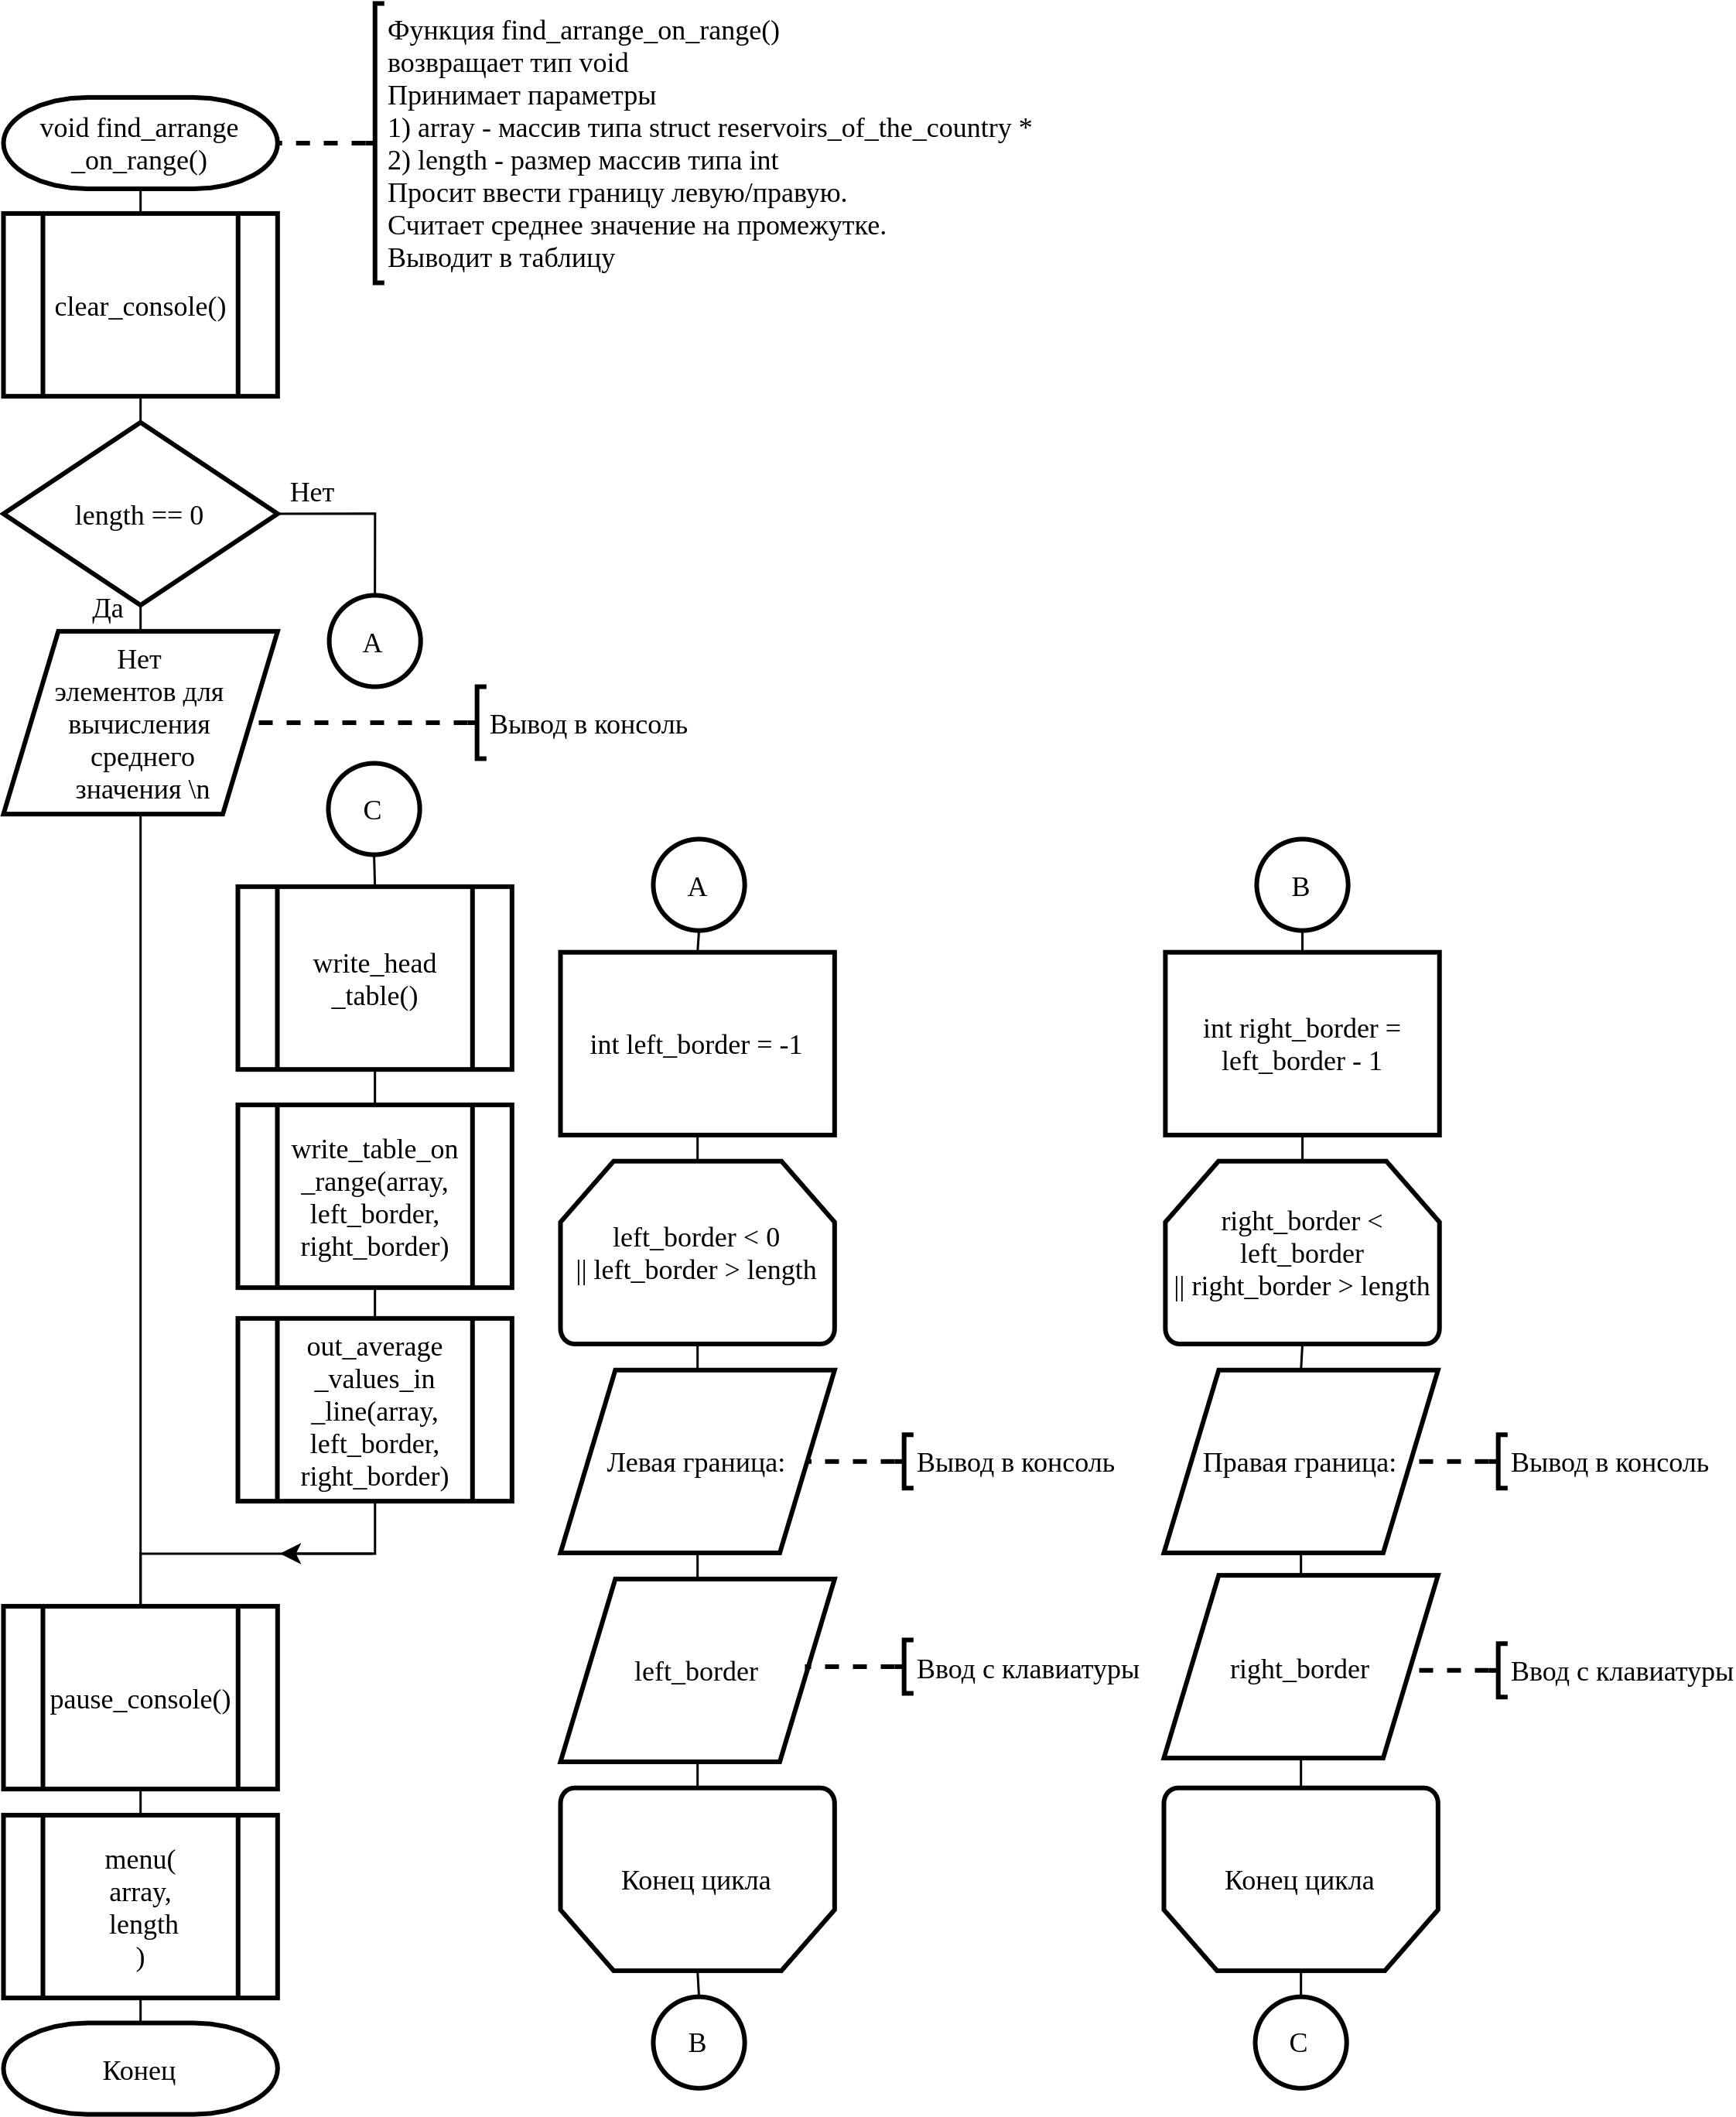
\includegraphics[width=16cm]{../src/app/menu/find_arrange_on_range/find_arrange_on_range.png}
    }
    \caption{find\_arrange\_on\_range()}
\end{figure}

% = = =

\label{link:lastPage}

\end{document}